% Create a one-sided article document type
\documentclass[a4paper, twoside, 12pt]{article}

% Define the course variables that are gonna be used several times
\newcommand{\university}{Universidad\ Politécnica\ de\ Madrid}
\newcommand{\school}{Escuela\ Técnica\ Superior\ de\ Ingenieros Informáticos}
\newcommand{\degree}{Grado\ Universitario\ en\ Ingeniería Informática}    
\newcommand{\tfg}{Trabajo de Fin de Grado}
\newcommand{\name}{Transformación de los datos de licitaciones de la Plataforma de Contratación Pública al estándar OCDS y su publicación como datos enlazados}
\newcommand{\me}{Pablo Palomo López}
\newcommand{\tutor}{María Poveda Villalón}
\newcommand{\supervisor}{Óscar Corcho García}

% Configure the metadata of the PDF document
\usepackage[
	bookmarks       = true,             % Show the bookmarks
	unicode         = true,             % Use Unicode                 
	pdftoolbar      = true,             % Show Acrobat’s toolbar
	pdfmenubar      = true,             % Show Acrobat’s menu
	pdffitwindow    = false,            % Window fit to page when opened
	pdfstartview    = {FitH},           % Fit the page width to the window
	pdfauthor       = {\me},            % The author of this document
	pdftitle        = {\name\ --\ \me}, % The title of this document
	pdfsubject      = {\name},          % The subject of this document
	pdfkeywords     = {\name},          % The keywords of this document
	pdfnewwindow    = true,             % Open the links in a new PDF window
	colorlinks      = true,             % Use colored links
	linkcolor       = blue,             % Internal links color
	citecolor       = blue,             % Bibliographic links color
	filecolor       = blue,             % File links color
	urlcolor        = blue              % External links color
]{hyperref}
\pdfstringdefDisableCommands{\let\uppercase}

% Redefine the size and margins (delete the 'twoside' indentation)
\usepackage[a4paper]{geometry}
% Define the geometry of the document
\newgeometry {
    top = 2.2cm, 
    bottom = 2.2cm, 
    right = 2cm, 
    left = 2cm
}
% Use UTF-8 as input encoding
\usepackage[utf8]{inputenc}
% Use a modern font (that is not pixelated)
\usepackage{lmodern}
% Use microtype to improve readability
\usepackage[protrusion = true, expansion = true]{microtype} 
% Use multiple columns
\usepackage{multicol}
% Display list of Equations
\usepackage{tocloft}
% Insert empty pages
\usepackage{afterpage}

% Custom packages
% Font specification
\usepackage{fontspec}
\setmainfont[
    ItalicFont=NewCM10-Italic.otf,
    BoldFont=NewCM10-Bold.otf,
    BoldItalicFont=NewCM10-BoldItalic.otf,
    SmallCapsFeatures={Numbers=OldStyle}]
{NewCM10-Regular.otf}
\setsansfont[
    ItalicFont=NewCMSans10-Oblique.otf,
    BoldFont=NewCMSans10-Bold.otf,
    BoldItalicFont=NewCMSans10-BoldOblique.otf,
    SmallCapsFeatures={Numbers=OldStyle}]
{NewCMSans10-Regular.otf}
\setmonofont[
    Path=./fonts/,
    Extension=.ttf,
    BoldFont=*-SemiBold, % Semibold font as bold
    UprightFont=*-Regular, % Regular font as default
    ItalicFont=*-Medium, % Medium font as italic
    Scale=0.8]
{FiraCode}

% Graphic package for bullet points
\usepackage{graphicx}

% Hyperlinks
\PassOptionsToPackage{obeyspaces}{url}
\usepackage{breakurl}
\usepackage{hyperref}
\hypersetup{
    breaklinks=true,
    colorlinks=true,
    filecolor=magenta, 
    linkcolor=blue,
    urlcolor=blue,
}
\urlstyle{same}

% Colour definitions
\usepackage[dvipsnames]{xcolor}
\definecolor{DarkGray}{rgb}{0.4,0.4,0.4}
\definecolor{DarkGreen}{rgb}{0.0,0.34,0.25}
\definecolor{DarkRed}{rgb}{0.42,0.07,0.02}
\definecolor{DarkViolet}{rgb}{0.4,0.0,0.4}

% Language highlighting
\usepackage{listings}
\lstdefinelanguage{lXML}{
    alsoletter={-},
    basicstyle=\ttfamily,
    breaklines=true,
    breakatwhitespace=true,
    frame=single,
    gobble=19,
    keywordstyle=[1]{\bfseries\color{RoyalBlue}},
    keywordstyle=[2]{\itshape\color{PineGreen}},
    keywordstyle=[3]{\color{RedViolet}},
    keywords=[1]{cac, cbc, cac-place-ext, cbc-place-ext},
    morekeywords=[2]{
        AddressLine,
        Attachment,
        AuctionConstraintIndicator,
        AuctionTerms,
        AwardDate,
        AwardedTenderedProject,
        BudgetAmount,
        CityName,
        Contact,
        Contract,
        Country,
        Description,
        ElectronicMail,
        EstimatedOverallContractAmount,
        ExternalReference,
        ContractFolderID,
        ContractFolderStatus,
        ContractFolderStatusCode,
        ContractingSystemCode,
        DurationMeasure,
        EndDate,
        ID,
        IdentificationCode,
        ItemClassificationCode,
        Language,
        LegalDocumentReference,
        LegalMonetaryTotal,
        Line,
        LocatedContractingParty,
        Name,
        Party,
        PartyName,
        PartyIdentification,
        PayableAmount,
        PlannedPeriod,
        PostalAddress,
        PostalZone,
        ProcedureCode,
        ProcurementProject,
        ProcurementProjectLot,
        ProcurementProjectLotID,
        ReceivedTenderQuantity,
        RequiredCommodityClassification,
        ResultCode,
        StartDate,
        SubmissionMethodCode,
        Telefax,
        Telephone,
        TenderingProcess,
        TenderingTerms,
        TenderResult,
        TotalAmount,
        TypeCode,
        URI,
        WebsiteURI,
        WinningParty
    },
    morekeywords=[3]{
        currencyID,
        languageID,
        listURI,
        schemeName,
        unitCode
    },
    morestring=*[d]{"},
    morestring=[s][]{\#\{}{\}},
    rulecolor=\color{black},
    showstringspaces=false,
    stringstyle=\color{OrangeRed},
    tabsize=10
}
\lstdefinelanguage{lXML2}{
    alsoletter={.,:,/,-,\#},
    basicstyle=\ttfamily,
    breaklines=true,
    breakatwhitespace=true,
    frame=single,
    gobble=19,
    keywordstyle=[1]{\color{Cerulean}},
    keywordstyle=[2]{\color{ForestGreen}},
    keywordstyle=[3]{\color{BrickRed}},
    keywords=[1]{
        http://dbpedia.org/resource/Spain
    },
    morekeywords=[2]{
        http://www.w3.org/1999/02/22-rdf-syntax-ns\#type,
        http://dbpedia.org/ontology/currencyCode,
        http://www.w3.org/2002/07/owl\#sameAs
    },
    morekeywords=[3]{
        http://schema.org/Country,
        EUR,
        http://openei.org/resources/Spain
    },
    rulecolor=\color{black},
    tabsize=10
}
\lstdefinelanguage{lJSON}{
    alsoletter={\{,\},\[,\]},
    basicstyle=\ttfamily,
    breaklines=true,
    breakatwhitespace=true,
    frame=single,
    gobble=19,
    keywordstyle=[1]{\bfseries},
    keywordstyle=[2]{\color{Brown}},
    keywordstyle=[3]{\color{Red}},
    keywords=[1]{\{,\},\[,\]},
    morekeywords=[2]{
        awards,
        contracts,
        parties,
        planning,
        tender
    },
    morekeywords=[3]{
        additionalIdentifiers,
        address,
        amount,
        budget,
        classification,
        contactPoint,
        countryName,
        currency,
        date,
        description_es,
        documents,
        documentType,
        email,
        endDate,
        faxNumber,
        id,
        identifier,
        items,
        locality,
        lots,
        mainProcurementCategory,
        name,
        ocid,
        period,
        postalCode,
        procurementMethod,
        procurementMethodDetails_es,
        relatedLot,
        roles,
        schema,
        startDate,
        streetAddress,
        submissionMethod,
        submissionMethodDetails,
        suppliers,
        tag,
        telephone,
        tenderPeriod,
        title,
        url,
        value
    },
    morestring=*[d]{"},
    morestring=[s][]{\#\{}{\}},
    rulecolor=\color{black},
    showstringspaces=false,
    stringstyle=\color{BrickRed},
    tabsize=10
}
\lstdefinelanguage{lCSharp}{
    basicstyle=\ttfamily\small,
    breaklines=true,
    breakatwhitespace=true,
    commentstyle=\color{DarkViolet},
    escapeinside={(*@}{@*)},
    frame=single,
    gobble=14,
    keywordstyle=[1]{\textit},
    keywordstyle=[2]{\color{DarkGreen}},
    keywordstyle=[3]{\color{DarkRed}},
    keywordstyle=[4]{\color{PineGreen}},
    keywords=[1]{
        from,
        enum,
        get,
        in,
        interface,
        namespace,
        null,
        public,
        select,
        set,
        where
    },
    morekeywords=[2]{
        AsyncCollection,
        Document,
        EPackagerOperationCode,
        EProviderOperationCode,
        IDictionary,
        IEnumerable,
        IMapper,
        IPackager,
        IParser,
        IProvider,
        LocalName,
        Name,
        JObject,
        string,
        Task,
        Thread,
        Uri,
        void,
        XElement,
        XName,
        XNamespace
    },
    morekeywords=[3]{
        AllProvider,
        Commit,
        Files,
        DocumentRoot,
        Elements,
        EntryRoot,
        Equals,
        GetDocumentTimestamp,
        GetElements,
        GetEntrySet,
        GetIdentifier,
        GetNamespaces,
        GetNextFile,
        MapElement,
        MappedEntry,
        Package,
        Parser,
        Publish,
        PROVIDE_ALL,
        PROVIDE_LATEST,
        PROVIDE_SPECIFIC,
        SetEntryRootElement,
        SetParser,
        RemoveFile,
        TakeFile
    },
    morekeywords=[4]{
        code,
        dirPath,
        document,
        entry,
        entryID,
        filePath,
        namespaces,
        node,
        parsedElement,
        pathMap,
        pathToElement,
        parser,
        publishDate,
        query,
    },
    morecomment=[l]{//}, 
    morecomment=[l]{///},
    morecomment=[s]{/*}{*/},
    morestring=*[d]{"},
    morestring=[s][]{\#\{}{\}},
    sensitive=true,
    showspaces=false,
    showstringspaces=false,
    stringstyle=\color{BrickRed},
    tabsize=10
}
\lstdefinelanguage{lSPARQL}{
    alsoletter={@},
    basicstyle=\ttfamily,
    breaklines=true,
    breakatwhitespace=true,
    frame=single,
    gobble=19,
    keywordstyle=[1]{\bfseries\color{DarkGray}},
    keywordstyle=[2]{\itshape\color{DarkGray}},
    keywords=[1]{
        OPTIONAL,
        @prefix,
        SELECT,
        WHERE,
    },
    morekeywords=[2]{
        dc,
        ocds,
        ocdsext,
        org,
        rdf,
        schema,
        skos,
        tbfy
    },
    morestring=[s]{<}{>},
    rulecolor=\color{black},
    stringstyle=\color{black},
    tabsize=10
}
% Fixed tabbing
\usepackage{tabto}

% Section label commands
\usepackage{nameref}
\newcommand{\currentsection}{}
\newcommand{\mysection}[1]{\section{#1}\renewcommand{\currentsection}{#1}}

% Sections depth
\usepackage{titlesec}
\setcounter{secnumdepth}{4}
\setcounter{tocdepth}{3}

% Table centered wrapping
\usepackage{array}
\newcolumntype{P}[1]{>{\centering\arraybackslash}p{#1}} %% horizontal centering
\newcolumntype{M}[1]{>{\centering\arraybackslash}m{#1}} %% vertical centering

% Multipage tables
\usepackage{longtable}

% Indexes name change
\renewcommand*\contentsname{Índice}
\renewcommand*\listtablename{Índice de tablas}
\renewcommand*\listfigurename{Índice de figuras}

% Subitem bullets style
\renewcommand{\labelitemii}{\circ}
\renewcommand{\labelitemiii}{\diamond}

% Configure style aspects of the document
\usepackage{caption}            % To configure the captions
\usepackage{siunitx}            % For SI units
\usepackage{graphicx}           % To include graphics
\usepackage{subcaption}         % To include subgraphics
\graphicspath{
    {schemes/} {images/}        % Images folder path
}
\usepackage[dvipsnames]{xcolor} % To configure colors
\usepackage{fancyhdr}           % To configure the header and footer
\pagestyle{fancy}               % Use a fancy header style
\fancyhf{}                      % Set the header format
\fancyheadoffset{0.0 cm}        % Set the header offset
\lhead{\tfg}                    % Set the header left-side contents
\rhead{\currentsection}         % Set the header right-side contents
\cfoot{\thepage}                % Set the footer page number

% Label changes
\captionsetup[table]{name=Tabla}
\captionsetup[figure]{name=Figura}

% Create a custom command shortcut
\renewcommand{\arraystretch}{1.3} % Modify the vertical spacing of the tables
\raggedbottom                     % Modify the vertical spacing of enumerated environments

% Set empty page 
\newcommand\blankpage{%
    \null
    \thispagestyle{empty}%
    \addtocounter{page}{-1}%
    \newpage
}

% Set the title format
\title {
	\vspace*{1.0 cm}
	\Large\textbf{\uppercase{\university}} \\
	\vspace*{0.5 cm}
	\large\textbf{\uppercase{\school}} \\
	\vspace*{2 cm}
	\large\text{\uppercase{\degree}} \\
	\vspace*{2 cm}
	\large\text{\uppercase{\tfg}} \\
	\vspace*{1.0 cm}
	\LARGE\textbf{\uppercase{\name}} \\
}

% Set the author format
\author {
	\normalsize
	\begin{tabbing}
        \hspace*{0.4\linewidth} \= \hspace*{0.5\linewidth} \= \kill
    	\> Autor: \' \textbf{\me} \\[0.25cm]
    	\> Tutora: \' \textbf{\tutor} \\[0.25cm]
    	\> Supervisor: \' \textbf{\supervisor} \\
    \end{tabbing}
    
    \vspace{2cm}
}

% Set the date format
\date { 
    Madrid, mayo de 2021
}

% A macro to print the title
\makeatletter
\def\printtitle{{\centering\@title\par}}
\makeatother

% A macro to print the author
\makeatletter
\def\printauthor{{\centering\large\@author}}
\makeatother

% A macro to print the date
\makeatletter
\def\printdate{{\centering\@date}}
\makeatother

%%%%%%%%%%%%%%%%%%%%%%%%%%%%%%%%%%%%%%%%%%%%%%%%%%%%%%%
% Start the document
\begin{document}
    % Include the cover
    \afterpage{\blankpage}
    \thispagestyle{empty} % Remove page numbering on this page

\begin{center}
    
    \centering
    \begin{figure}[h!]
        \centering
        \begin{subfigure}
            \centering
            % Include UPM's logo
        	
\includegraphics[width = 0.5\linewidth, height = 3cm, keepaspectratio]{images/UPM.eps}
    	\end{subfigure}
    	\hspace{3cm}%
    	\centering
        \begin{subfigure}
            \centering
            % Include ETSII's logo
        	
\includegraphics[width = 0.5\linewidth, height = 3cm, keepaspectratio]{images/ETSII.eps}
        \end{subfigure}
	\end{figure}
	
	% Print the title
	\printtitle
	
	% Add vertical padding
    \vfill
    
    % Print the author
    \printauthor
    
    % Print the date
    \printdate
\end{center}

\newpage              % Insert a page break
\setcounter{page}{1}  % Set the page counter
    % Include the different sections
    \pagenumbering{roman}
    \addtocounter{page}{-1}

\vspace*{15em}
\section*{Abstract}
    \vspace{0.5cm}
    \begin{adjustwidth}{50pt}{50pt}
        \hspace{15pt} This paper explores both the current  publication state of the contracting data at national and European levels, as well as the methodologies of said publications: open and linked data. In addition, the two reference standards, \texttt{CODICE} and \texttt{OCDS}, are presented.
        \\ \\
        \indent Next, the developed software whose purpose is to execute the data transformation between the two standards, is presented. The implemented mappings are listed in the following section.
        \\ \\
        \indent Finally, the way system produced data is published as open linked data through the software deployment is described.
    \end{adjustwidth}
    \vspace{1cm}
    \hspace{0.5cm} \textbf{\textit{Keywords}}: public contracting, tender, open data, linked data, standard.

\phantomsection
\addcontentsline{toc}{section}{Abstract}

\newpage
    \vspace*{15em}

\begin{center}
    \section*{Resumen}
    
        ...

\end{center}

\phantomsection
\addcontentsline{toc}{section}{Resumen}

\newpage
    \vspace*{5em}

\begin{center}
    \section*{Agradecimientos}
    
        \begin{adjustwidth}{-1pt}{-1pt}
             \begin{flushright}
                \textit{A mi tutora María y a mi supervisor Óscar,
                \\
                por transmitirme el entusiasmo necesario para realizar este trabajo.}
            \end{flushright}
        
            \vspace{1cm}
        
            \begin{flushright}
                \textit{A mis padres,
                \\
                por todo su esfuerzo y dedicación para brindarme la mejor educación posible.}
            \end{flushright}
            
            \vspace{1cm}
            
            \begin{flushright}
                \textit{A mi hermana Lydia por su siempre desinteresada ayuda 
                \\
                para ilustrar o referenciar mis trabajos y proyectos.}
            \end{flushright}
            
            \vspace{1cm}
            
            \begin{flushright}
                \textit{A los amigos que me llevo de la carrera;
                \\
                a Álex, Dani, a Diana, a Iván, a Raúl.}
            \end{flushright}
            
            \vspace{1cm}
            
            \begin{flushright}
                \textit{A quienes han estado conmigo todos estos años;
                \\
                \small{a Andrés, a Arturo, a Carlos, a Esther, a Guille, a Jaime, a Laura, a Luna, a Miguel, a Sara, a Tomás.}}
            \end{flushright}
            
            \vspace{1cm}
            
            \begin{flushright}
                \textit{Y a los que siempre me han acompañado.}
                \\ \vspace{0.2cm}
                
\includegraphics[width=0.1\textwidth]{pets.png}
            \end{flushright}
        \end{adjustwidth}
\end{center}

\phantomsection
\addcontentsline{toc}{section}{Agradecimientos}

\newpage
    \tableofcontents

\newpage
    {%
    \let\oldnumberline\numberline%
    \renewcommand{\numberline}{Tabla~\oldnumberline}%
    \listoftables%
}
    {%
    \let\oldnumberline\numberline%
    \renewcommand{\numberline}{Figura~\oldnumberline}%
    \vspace{1cm}
    \listoffigures%
}

\newpage

    \pagenumbering{arabic}
    \section{Introducción}

...

\newpage
    \mysection{Estado del arte}

    \subsection{Datos abiertos y datos enlazados}
        Para poder valorar este proyecto, es fundamental comprender las bases sobre las que se sustenta el mismo: los datos abiertos y los datos enlazados.
        \\  \\
        Los datos abiertos (\textit{open data}, en inglés) son datos que pueden ser utilizados, reutilizados y redistribuidos libremente por cualquier persona, y que se encuentran sujetos, a lo sumo, al requerimiento de atribución y de compartirse de la misma manera que aparecen.
        \\ \\
        Sin embargo, más allá de las propiedades que los datos abiertos deben satisfacer (disponibilidad, accesibilidad, reutilización, redistribución y participación universal), el valor de estos datos es la interoperabilidad. La interoperabilidad denota la habilidad de diversos sistemas y organizaciones para trabajar en conjunto. En este escenario, nos referimos a la cualidad de integrar diferentes conjuntos de datos \cite{OPENDATA}.
        \\ \\
        Gracias a la interoperabilidad de los datos abiertos, se pueden construir \hyperref[sec:software]{sistemas} como los que se describirán en este trabajo posteriormente, capaces de reutilizar los datos publicados por una fuente y transportarlos a otro dominio, con el objetivo de explotar la información a través de nuevas vías.
        \\ \\
        Por otro lado, los datos enlazados (\textit{linked data}, en inglés) son la base de la denominada \textit{Web Semántica}. La peculiaridad de esta información reside en la referenciación: mediante dicho mecanismo, los datos pueden vincularse entre ellos de la misma manera que lo hacen los enlaces de las páginas web \cite{LINKEDDATA}.
        \\ \\
        
        \begin{figure}[h]
            \centering
            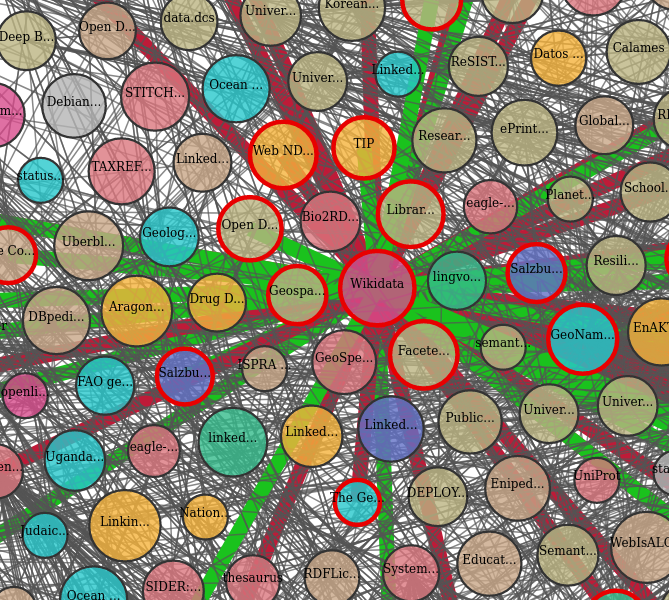
\includegraphics[width=0.625\textwidth]{lod_zoom.png}
            \captionof{figure}{Zoom de la \textit{Linked Open Data Cloud}}
            \label{fig:lod}
        \end{figure}
        
        \noindent En la \hyperref[fig:lod]{figura 1} se puede apreciar una pequeña parte de la \textit{Linked Open Data Cloud} \cite{LOD}, que refleja todos los conjuntos de datos abiertos y enlazados publicados, así como las relaciones entre los mismos. Esta inmensa ``nube" evidencia el poder y el valor de esta forma de publicación de datos, capaz de conformar una red de conocimiento muy amplia.
        \\ \\
        A diferencia de otros modelos de almacenamiento y gestión de la información, como las bases de datos convencionales, en los que se necesitan mecanismos auxiliares para reflejar esta referenciación e interconexión de datos, los datos enlazados poseen de manera intrínseca estas relaciones. Esta diferencia radica en la forma en la que se describen los datos: la web del hipertexto, la que estamos acostumbrados a explorar, suele estar descrita mediante el lenguaje \texttt{HTML} (por sus siglas en inglés, \textit{HyperText Markup Language} \cite{HTML}), mientras que la \textit{Web Semántica} se describe mediante el modelo \texttt{RDF} (\textit{Resource Description Framework}, en inglés \cite{RDF}).
        \\ \\
        
        \begin{figure}[h]
            \centering
            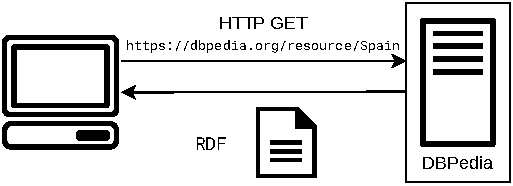
\includegraphics[]{linked.pdf}
            \captionof{figure}{Ejemplo de una consulta de datos enlazados}
            \label{fig:linked}
        \end{figure}

        \noindent A modo de ejemplo, y con el objetivo de reflejar algunos de los principios básicos de los datos enlazados, se muestra en la \hyperref[fig:linked]{figura 2} un caso de uso de una consulta sobre datos enlazados. La consulta es simple: un equipo solicita el recurso que representa la entidad de España al servidor de \textit{DBpedia} \cite{DBPEDIA}, uno de los proyectos más ambiciosos de la \textit{Web Semántica}, que busca extraer la información de la más amplia enciclopedia \textit{online}, \textit{Wikipedia}, para generar datos enlazados.
        \\ \\
        En el ejemplo se pueden ver algunas de las peculiaridades de los datos enlazados:
        \begin{itemize}
            \item Uso de \texttt{URI}s como identificadores: con el objetivo de evitar ambigüedades y poder ofrecer una forma estandarizada y unívoca de identificación de entidades, todos los recursos se identifican mediante una \texttt{URI} (por su traducción del inglés, Identificador de recursos uniforme). Por lo tanto, una \texttt{URI} no es sólo una dirección, sino también un identificador: en el ejemplo, \texttt{\url{https://dbpedia.org/resource/Spain}} es la dirección en la que se aloja el recurso, pero también es el identificador que permite a cualquier otro sistema reutilizar dicho recurso.
            \item Protocolo \texttt{HTTP}: para evitar la multiplicidad de esquemas de \texttt{URI}s, se utiliza \texttt{HTTP} para asegurar que cualquier recurso pueda ser buscado y accedido en la Web.
            \item Obtención de recursos mediante \texttt{RDF}: Una vez se ha realizado una búsqueda y se pretende acceder a un recurso identificado por su \texttt{URI}, se obtiene una respuesta en forma de documento en formato \texttt{RDF}, que será explicado con más precisión en la \hyperref[subsubsec:RDF]{posterior sección}. Además, la forma de realizar consultas estructuradas sobre datos enlazados más allá de su obtención mediante \texttt{URI}s será descrita en \hyperref[subsubsec:SPARQL]{la última subsección}.
        \end{itemize}
        
        \subsubsection{Modelo de datos \texttt{RDF}} \label{subsubsec:RDF}
            Si bien debido a la comparación previa entre la Web estándar y la denominada \textit{Web Semántica} podría parecer que \texttt{RDF} es un lenguaje de marcado de texto como lo es \texttt{HTML}, esto no es así: \texttt{RDF} es un \textit{framework} de representación de información: un modelo que permite codificar la información, sus propiedades, y las relaciones entre sí.
            \\ \\
            La sintaxis de este modelo es simple: se basa en conjuntos de tripletas de la forma sujeto-predicado-objeto, donde éstos pueden ser \texttt{URI}s, literales o elementos vacíos. Mediante estos conjuntos de definiciones se pueden construir \textit{datasets}, que a su vez se pueden organizar en grafos de conocimiento; estructuras con una alta riqueza en términos de información.
            \\ \\
            
            \begin{lstlisting}[language=lXML2,gobble=14]
                <http://dbpedia.org/resource/Spain>
                    <http://www.w3.org/1999/02/22-rdf-syntax-ns#type>	
                    <http://schema.org/Country> .
                <http://dbpedia.org/resource/Spain>
                    <http://dbpedia.org/ontology/currencyCode>
                    "EUR" .
                <http://dbpedia.org/resource/Spain>
                    <http://www.w3.org/2002/07/owl#sameAs>
                    <http://openei.org/resources/Spain> .
            \end{lstlisting}
            \captionof{figure}{Ejemplo de tripletas del modelo \texttt{RDF}}
            \label{fig:triplets}
            
            \vspace{0.7cm}
            
            En la \hyperref[fig:triplets]{figura 3} se pueden apreciar algunas de las tripletas que se otorgarían como respuesta a una petición como la de la \hyperref[fig:linked]{figura 2}. En \textcolor{Cerulean}{azul} aparecen los sujetos de las tripletas, mientras que en \textcolor{ForestGreen}{verde} y en \textcolor{BrickRed}{rojo} aparecen los predicados y los objetos, respectivamente.
            \\ \\
            La información de las tripletas, como se explicó previamente, está codificada mediante \texttt{URI}s, nodos vacíos o literales que representan entidades, propiedades y relaciones. En este caso, la primera tripleta nos dice que la entidad que representa a España es de tipo (\textcolor{ForestGreen}{\texttt{type}}) país (\textcolor{BrickRed}{\texttt{Country}}). La segunda, que en España el tipo de moneda (\textcolor{ForestGreen}{\texttt{currencyCode}}) tiene un código (\textcolor{BrickRed}{\texttt{EUR}}), que es un literal. La última de ellas establece una relación de identidad (\textcolor{ForestGreen}{\texttt{sameAs}}) entre el recurso \textcolor{Cerulean}{\texttt{http://dbpedia.org/resource/Spain}} y el recurso \textcolor{BrickRed}{\texttt{http://openei.org/resources/Spain}}, que se encuentran en distintos dominios.
            \\ \\
            En este ejemplo también pueden ser destacados otros elementos característicos de \texttt{RDF}: los vocabularios. Para expresar las propiedades (como \textcolor{ForestGreen}{\texttt{type}} o \textcolor{ForestGreen}{\texttt{sameAs}}), que potencialmente pueden aparecer en múltiples \textit{datasets}, es de interés poder contar con un índice de términos que poder reutilizar, siguiendo uno de los principios fundamentales de los datos abiertos y enlazados. Ésa es la función de proyectos como \textit{Linked Open Vocabularies} \cite{LOV}, que recoge a modo de códice todos los términos publicados como datos abiertos.
            \\ \\
            Un último apunte sobre \texttt{RDF} y el ejemplo provisto; como previamente se explicó sobre \texttt{RML}, éste no es un lenguaje de marcado sino un \textit{framework} que refleja cómo deben de ser los datos enlazados para que sigan los principios que los rigen. El ejemplo de la \hyperref[fig:linked]{figura 3} está codificado mediante el formato \texttt{N-Triples} \cite{NTRIPLES} (un subconjunto del formato \texttt{Turtle} \cite{TURTLE}). Sin embargo, existen otros formatos, como \texttt{JSON-LD} \cite{JSONLD}, \texttt{RDF/XML} \cite{RDFXML}, \texttt{RDFa} \cite{RDFA} o \texttt{N-Quads} \cite{NQUADS}.
        
        \subsubsection{Consultas sobre datos enlazados} \label{subsubsec:SPARQL}
            De la misma manera que para la realización de consultas sobre bases de datos convencionales se tiene el lenguaje \texttt{SQL} \cite{ISOSQL}, para construir búsquedas estructuradas sobre grafos de conocimiento de datos enlazados se utiliza \texttt{SPARQL} \cite{SPARQL}.
            \\ \\
            \texttt{SPARQL} trabaja con los datos en formato \texttt{RDF} y contiene las capacidades para la consulta de los patrones obligatorios y opcionales de grafo, junto con sus conjunciones y disyunciones. La sintaxis de \texttt{SPARQL} es similar a la de su análogo de bases de datos relacionales; en la \hyperref[fig:sqlsparql]{figura 4} se puede apreciar una consulta similar mediante los dos lenguajes:
            \\ \\
        
            \begin{figure}[h]
                \centering
                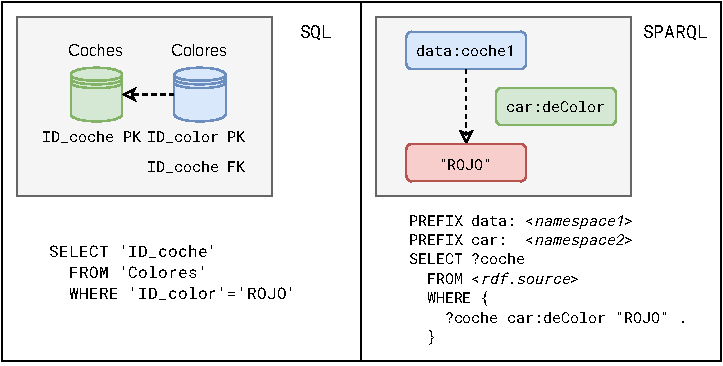
\includegraphics[]{sqlsparql.pdf}
                \captionof{figure}{Ejemplo de consultas en lenguajes \texttt{SQL} y \texttt{SPARQL}}
                \label{fig:sqlsparql}
            \end{figure}
            
            \noindent Las dos consultas muestran similitudes en distintos aspectos, como las cláusulas (\texttt{SELECT}, \texttt{FROM}, \texttt{WHERE}...) o la estructura de la sentencia, pero también evidencian las diferencias entre los lenguajes y los modelos tanto de bases de datos relacionales, como el modelo \texttt{RDF}: las consultas \texttt{SQL} se realizan sobre unos datos estructurados y sus atributos, teniendo que conocer por anticipado dicha estructura para poder construir la sentencia. En cambio, mediante \texttt{SPARQL} se pueden consultar directamente las tripletas del conjunto de datos. Además, este protocolo permite el uso de prefijos para ejecutar las consultas sobre elementos en dominios diversos.
            \\ \\
            Existen diversos sistemas que implementan, mediante \textit{API}s o \textit{triplestores} (un tipo de base de datos \textit{ad-hoc} para datos enlazados), sistemas con mecanismos de construcción de consultas \texttt{SPARQL}. Algunas de dichas implementaciones son:
            \\
            \begin{itemize}
                \item Apache Jena \cite{JENA}: \textit{framework} de código abierto escrito en el lenguaje \texttt{Java} para el desarrollo de aplicaciones sobre datos \texttt{RDF}.
                \item RDFLib \cite{RDFLIB}: biblioteca en \texttt{Python} para el procesado de datos en formato \texttt{RDF/XML} y sus grafos de conocimiento asociados. Utilizada  \hyperref[subsec:rdflib]{posteriormente} en el trabajo.
                \item RDF4J \cite{RDF4J}: previamente conocido como \textit{OpenRDF Sesame}, es otro \textit{framework} de código abierto escrito en el lenguaje \texttt{Java}.
                \item Virtuoso \cite{VIRTUOSO}: \textit{middleware} que combina las funcionalidades de un gestor de bases de datos relacionales convencionales con el procesado de datos enlazados.
            \end{itemize}
        
    \subsection{Licitaciones públicas}
        \subsubsection{Estándar \texttt{CODICE}}
            \texttt{CODICE} es una librería de componentes y documentos electrónicos \texttt{XML} estándar para el desarrollo de aplicaciones de contratación pública electrónica de conformidad con los procedimientos y prescripciones de las directivas \texttt{2014/23/UE} \cite{UE201423}; \texttt{2014/24/UE} \cite{UE201424}; \texttt{2014/25/UE} \cite{UE201425}; \texttt{2009/81/CE} \cite{UE200981} y de la normativa española en materia de contratación pública \cite{BOE20179}, así como con los estándares y recomendaciones internacionales aplicables a la identificación, denominación, definición y construcción de dichos componentes.
            \\ \\
            El proyecto \texttt{CODICE} persigue proporcionar a todo el Sector Público una arquitectura de componentes, documentos y mensajes \texttt{XML} estandarizados, conforme con las normas y estándares internacionales aplicables, que pueda ser usada por todos los sistemas, aplicaciones y componentes informáticos necesarios para la construcción de soluciones interoperables de contratación electrónica.
            \\ \\
            La finalidad del proyecto es asegurar la interoperabilidad, tanto de los subsistemas de contratación electrónica entre sí (Plataforma de Contratación Pública, registros electrónicos de empresas, catálogos electrónicos, sistemas de subastas electrónicas, etc.), como con los sistemas de información de los agentes económicos participantes en los procesos de contratación y con los de los propios órganos de las Administraciones Públicas.
            \\
        
            \begin{figure}[h]
                \centering
                
\includegraphics[width=\textwidth]{codice.png}
                \captionof{figure}{Logo del estándar \texttt{CODICE} (versión 2)}
            \end{figure}
            
            \noindent Para acomodar de forma armónica y coordinada las variadas necesidades y condicionantes de los distintos usuarios potenciales de los sistemas de contratación electrónica a desplegar, así como para facilitar la interoperabilidad de la plataforma de contratación pública y sus distintos subsistemas con las infraestructuras técnicas, organizativas y de información de todos los participantes en los procesos de contratación pública, se ha definido una arquitectura \cite{CODICEIMPL} que proporciona tanto los componentes comunes esenciales del sistema (definiciones y denominaciones normalizadas, componentes o módulos elementales reutilizables, documentos electrónicos de uso común, etc.), como la estructura y reglas que permite su extensión o adaptación a las necesidades especiales de diferentes contextos específicos de contratación.
            \\ \\
            Dicha arquitectura proporciona a los sistemas a desarrollar posteriormente los “bloques” o componentes básicos de información, así como las reglas de composición necesarias para la construcción de los documentos y mensajes electrónicos que licitadores y órganos de contratación han de intercambiarse a lo largo de los procesos de contratación, garantizando al mismo tiempo la interoperabilidad de todos los elementos cuya interacción proporcionará las funcionalidades necesarias para hacer efectiva la contratación electrónica \cite{CODICEFORM}.
            \\ \\
            Las normas y estándares internacionales existentes, tales como las normas ISO 11179 \cite{ISOMDR} y 15000 \cite{ISOEBXML}, los estándares ebXML de OASIS \cite{EBXML} y UN/CEFACT \cite{UNCEFACT}, y las Recomendaciones del W3C sobre lenguaje y esquema \texttt{XML} \cite{XML}, junto con las iniciativas promovidas por el programa IDA de la Unión Europea en relación con la contratación electrónica \cite{UEIDA}, han proporcionado la base para la definición y construcción de una arquitectura interoperable de información \cite{CODICE}.
            \\ \\
            En el portal institucional del Ministerio de Hacienda, concretamente en la sección de licitaciones publicadas en la Plataforma de Contratación del Sector Público \cite{PORTALHAC}, se pueden encontrar los documentos de licitaciones elaborados por la Dirección General del Patrimonio del Estado a partir de los datos que introducen los órganos de contratación como responsables de sus perfiles de contratantes. Estos documentos siguen el esquema \texttt{CODICE}, si bien no en todos los documentos van a aparecer los mismos elementos, dado que se proporcionan tres distintos tipos de documentos: licitaciones publicadas en la Plataforma de Contratación del Sector Público (excluyendo contratos menores), licitaciones publicadas mediante mecanismos de agregación y licitaciones correspondientes a contratos menores \cite{CODICETIPOS}. Este trabajo se ha centrado en el primero de los tipos previamente descritos, que incluye como superconjunto al tercero, el de los contratos menores.
            
        \subsubsection{Estándar \texttt{OCDS}}
            El Estándar de Datos para las Contrataciones Abiertas (\texttt{OCDS}, por sus siglas en inglés) permite la divulgación de datos y documentos de todas las etapas del proceso de contratación mediante la definición de un modelo de datos común. Se creó para apoyar a las organizaciones a aumentar la transparencia de la contratación y permitir un análisis más profundo de los datos de contrataciones por una amplia gama de usuarios.
        
            \begin{figure}[h]
                \centering
                
\includegraphics[width=0.575\textwidth]{ocds.png}
                \captionof{figure}{Logo del estándar \texttt{OCDS}}
            \end{figure}
            
            \noindent \texttt{OCDS} es un estándar de datos abierto, gratuito y no protegido por derechos de propiedad intelectual para la contratación pública, implementado por más de 30 gobiernos en todo el mundo. Es el único estándar abierto internacional para la publicación de información relacionada con la planeación, licitación e implementación de contratos públicos y ha sido avalado por el G20, el G7 e importantes organizaciones internacionales \cite{OCDS}.
            \\ \\
            \texttt{OCDS} describe cómo publicar datos y documentos en todas las etapas del proceso de contratación. Fue creado para brindar apoyo a las organizaciones con el objetivo de aumentar la transparencia en las contrataciones y permitir un análisis más exhaustivo de los datos sobre contrataciones por parte de una amplia variedad de usuarios. \texttt{OCDS} brinda:
            
            \begin{itemize}
                \item Una serie de campos de datos y documentos para publicación recomendados
                \item Un modelo de datos estructurado común
                \item Orientación y herramientas para la implementación y el uso de datos
                \item Perfiles para asociaciones público-privadas, proyectos de infraestructura, la Unión Europea y el Acuerdo sobre Contratación Pública de la Organización Mundial del Comercio
                \item Un mecanismo de extensión para incorporar información adicional clave a sus datos de \texttt{OCDS}
                \item Un servicio de asistencia global gratuito
            \end{itemize}
            
            \noindent Los datos sobre contrataciones publicados en un formato de \texttt{OCDS} resultan más fáciles de compartir, comparar y analizar. Permiten que quienes los publican adapten y reutilicen las herramientas existentes de visualización y análisis como éstas \cite{OCDSTOOLS}, lo cual reduce los costes y favorece la innovación. \texttt{OCDS} ofrece orientación sobre qué publicar y cómo publicar los detalles más importantes sobre contratación pública identificados por profesionales, investigadores y otras partes interesadas.
            \\ \\
            \texttt{OCDS} fue concebido para atender cuatro necesidades específicas de los usuarios, en función de un análisis campo por campo de cómo pueden utilizarse los datos para dar respuesta a tales necesidades. Estas son:
            
            \begin{itemize}
                \item Lograr mayores beneficios a cambio del dinero que se paga, con lo cual se permite que el gobierno ahorre tiempo y dinero.
                \item Generar un entorno de negocios más justo y condiciones equitativas para los proveedores.
                \item Mejorar la integridad pública al desalentar el fraude y la corrupción.
                \item Hacer un seguimiento de la prestación de los servicios y mejorarlos.
            \end{itemize}
            
            Si se incorporan a reformas más amplias, los gobiernos pueden utilizar las contrataciones abiertas para obtener mayores beneficios a cambio del dinero que se paga por los bienes, las obras y los servicios y para ganarse la confianza del sector privado, la sociedad civil y la ciudadanía \cite{OCDSOC}.
            \\
            
            \begin{figure}[h]
                \centering
                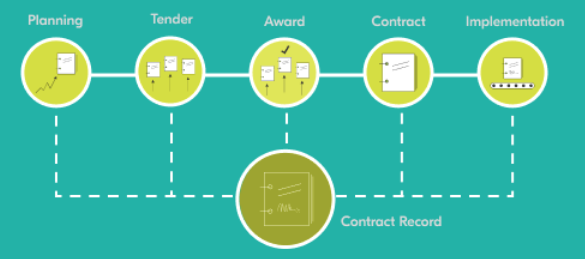
\includegraphics[width=0.67\textwidth]{tenderprocess.png}
                \captionof{figure}{Modelo del proceso de licitaciones en \texttt{OCDS}}
                \label{fig:tenderprocess}
            \end{figure}
            
            \noindent El proceso de licitaciones (véase \hyperref[fig:tenderprocess]{figura 7}), si bien sigue un modelo lineal, no siempre ha de cumplirse estrictamente de esa manera, dado que no todas las contrataciones pasan por todas las etapas, o en algunos casos es necesario proveer nueva información sobre una etapa previa.
            \\ \\
            Un documento \texttt{OCDS} está compuesto por bloques, íntegramente relacionados con el modelo del proceso de licitaciones \cite{OCDSBLOCKS}:
            
            \begin{itemize}
                \item \texttt{parties}: información sobre las organizaciones y otros participante involucrados en el proceso de contratación.
                \item \texttt{planning}: información sobre los objetivos, presupuestos y proyectos a los que se refiere un proceso de contratación.
                \item \texttt{tender}: información sobre la forma en que tendrá lugar la licitación o su realización.
                \item \texttt{awards}: información sobre las adjudicaciones otorgadas como parte de un proceso de contratación.
                \item \texttt{contracts}: información sobre contratos firmados como parte de un proceso de contratación.
                \begin{itemize}
                    \item \texttt{implementation}: información sobre el progreso de cada contrato hasta su finalización.
                \end{itemize}
            \end{itemize}
            
    \subsection{\textit{TheyBuyForYou}}
        \textit{TheyBuyForYou} (en adelante, \texttt{TBFY}) es un consorcio de empresas, universidades, centros de investigación, departamentos gubernamentales y autoridades locales de diversos países europeos, concretamente Reino Unido, Noruega, Italia, España y Eslovenia.
        \\ \\
        
        \begin{figure}[h]
            \centering
            
\includegraphics[width=0.5\textwidth]{tbfy.png}
            \captionof{figure}{Logo del proyecto \texttt{TBFY}}
        \end{figure}
        
        \noindent El proyecto de \texttt{TBFY} comenzó en enero de 2018 con el objetivo de mejorar el estado del mercado de adquisiciones europeo mediante el desarrollo de herramientas y funcionalidades que permitan explorar los datos abiertos en el ámbito de las licitaciones públicas. Para situarlo en contexto, ya hay diferentes organizaciones aprovechando el uso de las herramientas desarrolladas por el equipo de \texttt{TBFY}; el gobierno de Eslovenia las utiliza para identificar patrones que pudieran ser indicadores de fraude y autoridades españolas las usan para tomar decisiones de contrataciones más transparentes, entre otros casos.
        \\ \\
        El mercado de licitaciones europeo es tan grande que su navegación por parte de administraciones públicas, licitadores y empresas es complejas; es por ello que habitualmente grandes compañías consiguen contratos por encima de pequeños suministradores. \texttt{TBFY} quiere cambiar esto mediante la construcción de un gran grafo de conocimiento que recoja millones de datos sobre contrataciones públicas en el ámbito europeo. Siguiendo los principios que rigen los datos abiertos, los recursos de \texttt{TBFY} son públicos y de acceso abierto \cite{TBFY}.
        \\ \\
        
        \begin{figure}[h]
            \centering
            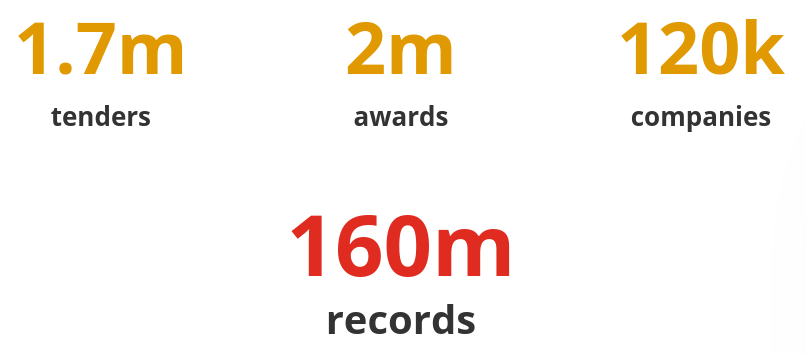
\includegraphics[width=0.625\textwidth]{tbfykg.png}
            \captionof{figure}{Dimensiones del grafo de conocimiento de \texttt{TBFY} (mayo de 2021)}
        \end{figure}
        
        \noindent Los datos recogidos en el grafo de conocimiento de \texttt{TBFY} son accesibles mediante \textit{endpoints} \texttt{SPARQL}, nodos sobre los cuales se pueden realizar peticiones mediante el protocolo \texttt{HTTP} y obtener respuestas en distintos formatos. Además, \texttt{TBFY} proporciona otras herramientas; el repositorio central \cite{TBFYREPOS}, una aplicación de búsquedas construida mediante \texttt{OptiqueVQS} (\textit{Visual Query System over Ontologies}) \cite{TBFYVQS}, una herramienta capaz de encontrar patrones anómalos en datos de contrataciones \cite{TBFYANOM}, etc.
        \\ \\
        Mediante el uso de la aplicación desarrollada en la \hyperref[sec:software]{posterior sección}, se generarán datos abiertos y enlazados capaces de ser explotados mediante algunas de las herramientas de \texttt{TBFY}.

\newpage
    \mysection{Software desarrollado} \label{sec:software}
    La presente sección describe el sistema software desarrollado, \textit{OCDS\_Mapper}, mediante el formato de un documento de diseño software (SDD, por sus siglas en inglés). En esta sección se proporcionar una visión general del sistema, desde su descripción hasta sus funcionalidades, de las que se derivan las características concretas que han sido implementadas.
    \\ \\
    La documentación del software que se describirá a continuación estará guiada por la norma \texttt{J-STD-016-1995} \cite{JSTD}, un estándar para el ciclo de vida de los procesos de desarrollo de software promulgado por dos de los organismos más relevantes en el área de las tecnologías de la información; la EIA (\textit{Electronic Industries Association}) y el IEEE (\textit{The Institute of Electrical and Electronics Engineers}).
    \\ \\
    En esta sección que especifica el diseño de la arquitectura del sistema previamente citado, se incluyen los siguientes apartados:
    \\
    \begin{itemize}
        \item Consideraciones de diseño
        \item Estructura de la aplicación
        \item Diseño de la arquitectura
        \item Diseño detallado del sistema
        \item Trazabilidad de requisitos
        \item Flujo de ejecución
        \item Cobertura de código
    \end{itemize}
    
    \subsection{Consideraciones de diseño}
        \subsubsection{Lenguaje de programación}
            La implementación del sistema se ha realizado mediante el \textit{framework} \texttt{.NET Core 5.0.202}, usando el lenguaje \texttt{C\#} bajo el estándar que describe su sintaxis e interpretación \cite{ISOCS}.
            
        \subsubsection{Arquitectura de componentes orientada a servicios}
            Con el objetivo de alcanzar la máxima abstracción de tareas posible, el sistema se ha diseñado de tal forma que cada componente realice un servicio concreto, con una funcionalidad bien definida, capaz de integrarse con el resto de componentes del sistema.
            \\ \\
            El \textit{OCDS\_Mapper}, por tanto, estará compuesto de componentes individuales, concretamente 4, descritos en la subsección \hyperref[subsubsec:componentes]{componentes software}.
            
        \subsubsection{Patrón de productor-consumidor}
            El sistema implementará el patrón de diseño software de productor-consumidor de la siguiente manera:
            \\ \\
            Las funcionalidades que implementen la recogida de datos, sea de manera local o remota, serán los productores, y las funcionalidades que implementen el procesado de los datos, esto es, el mapeado entre estándares, serán los consumidores.
            \\ \\
            Para asegurar un correcto flujo de recursos entre los componentes que sigan dichos roles se implementan mecanismos de sincronización y exclusión mutua entre ellos.
        
        \subsubsection{Mecanismo de consultas}
            Para realizar las búsquedas de elementos sobre los documentos de licitaciones de la Plataforma de Contratacíon Pública del Estado se ha utilizado la tecnología \textit{Language Integrated Query} (\texttt{LINQ}), propia del \textit{framework} \texttt{.NET}.
            \\ \\
            A través de \texttt{LINQ} se pueden realizar consultas sobre estructuras de datos mediante una sintaxis parecida a la del lenguaje \textit{Structured Query Language} (\texttt{SQL}). En concreto, para el tipo de datos que la aplicación obtiene (extensión \texttt{.atom}, formato \texttt{XML}), la rama de \texttt{LINQ} utilizada es \texttt{LINQ to XML} \cite{LINQXML}.
            \\ \\
            Para ejemplificar el funcionamiento de \texttt{LINQ}, se utilizará una sentencia utilizada en esta aplicación. Concretamente, el ejemplo provisto en la \hyperref[fig:linq]{figura 10} representa una consulta que busca el elemento raíz (\texttt{ContractFolderStatus}) de cada entrada de un documento de licitaciones.
            \\ \\
            \begin{lstlisting}[language=lCSharp,gobble=14]
                IEnumerable<XElement> query =
                    from node in entry.Elements()
                    where node.Name.LocalName.Equals("ContractFolderStatus")
                    select node;
            \end{lstlisting}
            \captionof{figure}{Ejemplo de una sentencia de \texttt{LINQ}}
            \label{fig:linq}
        
        \subsubsection{Librerías utilizadas} \label{subsubsec:libreria}
            El sistema utiliza distintas librerías para realizar la implementación de las funcionalidades requeridas. En concreto, estas librerías son:
            
            \begin{itemize}
                \item AsyncEx \cite{LIBASYNC}: Librería utilizada para el uso de colecciones aptas para la exclusión mutua. Licencia MIT \cite{LICMIT}.
                \item FluentAssertions \cite{LIBASSERT}: Librería de ayuda en la codificación de tests. Licencia Apache v2 \cite{LICAPACHE}.
                \item Microsoft.Extensions.Configuration \cite{LIBCONFIG}: Librería utilizada para pasar información a la aplicación mediante ficheros de configuración. Licencia MIT \cite{LICMIT}.
                \item NLog \cite{LIBNLOG}: Librería para llevar el registro del funcionamiento del sistema. Licencia BSD 3-Clause \cite{LICBSD3}.
                \item Json.NET \cite{LIBJSON}: Librería utilizada para la construcción de documentos en formato JSON. Licencia MIT \cite{LICMIT}.
                \item xUnit \cite{LIBXUNIT}: Librería para realizar el \textit{testing} del sistema. Liencia Apache v2 \cite{LICAPACHE}.
            \end{itemize}   
    
    \subsection{Estructura de la aplicación}
        La aplicación \textit{OCDS\_Mapper} (una \textit{solución}, en el ámbito de estructuras de proyectos en \textit{Visual Studio} \cite{VSPROJSOL}) está estructurada en dos \textit{proyectos}; \texttt{src} y \texttt{test}, con el código fuente del programa y el módulo de testeo de la aplicación, respectivamente. En la \hyperref[fig:estructura]{figura 11} se puede visualizar la estructura de directorios de la aplicación.
        \\ \\
        Además del fichero \texttt{Program.cs}, que incluye el punto de entrada de la aplicación, y el fichero de configuración \texttt{appsettings.json}, dentro del proyecto del código fuente de la aplicación se han estructurado los ficheros en los siguientes directorios:
        
        \begin{itemize}
            \item \texttt{Examples}: ejemplos de casos de uso de la aplicación.
                \begin{itemize}
                    \item \texttt{json}: ejemplos de documentos mapeados por la aplicación.
                    \item \texttt{xml}: ejemplos de documentos de la Plataforma de Contratación Pública.
                \end{itemize}
            \item \texttt{Exceptions}: excepciones propias del funcionamiento de la aplicación.
                \begin{itemize}
                    \item \texttt{EmptyMappingRuleException.cs}: se lanza si se provee una regla de mapeado vacía.
                    \item \texttt{InvalidOperationCodeException.cs}: se lanza si no se provee un modo de operación válido.
                    \item \texttt{InvalidParsedElementException.cs}: se lanza si no se encuentra el elemento raíz en una entrada de un documento de licitaciones.
                    \item \texttt{InvalidPathLengthException.cs}: se lanza si se provee una regla de mapeado de longitud inválida.
                    \item \texttt{WrongMappingException.cs}: se lanza si se encuentra un elemento inesperado en el mapeado de los datos.
                \end{itemize}
            \item \texttt{Interfaces}: interfaces de los componentes de la arquitectura.
                \begin{itemize}
                    \item \texttt{IMapper.cs}: interfaz del componente de mapeado de datos.
                    \item \texttt{IPackager.cs}: interfaz del componente de empaquetado de datos.
                    \item \texttt{IParser.cs}: interfaz del componente de parseo de datos.
                    \item \texttt{IProvider.cs}: interfaz del componente de provisión de datos.
                \end{itemize}
            \item \texttt{Model}: implementación de los componentes de la arquitectura.
                \begin{itemize}
                    \item \texttt{Mapper.cs}: implementación del componente de mapeado de datos.
                    \item \texttt{Packager.cs}: implementación del componente de empaquetado de datos.
                    \item \texttt{Parser.cs}: implementación del componente de parseo de datos.
                    \item \texttt{Provider.cs}: implementación del componente de provisión de datos.
                \end{itemize}
            \item \texttt{Utils}: ficheros con funcionalidades extra.
                \begin{itemize}
                    \item \texttt{Document.cs}: tipo de datos que abstrae una instancia de un documento de licitaciones.
                    \item \texttt{EnumCodes.cs}: fichero con los tipos enumerados del programa.
                    \item \texttt{Mappings.cs}: clase estática con las reglas de mapeado.
                \end{itemize}
        \end{itemize}
        
        En cuanto al proyecto de \textit{testing}, en los ficheros \texttt{UnitTests.cs} y \texttt{IntegrationTests.cs} se pueden encontrar las pruebas unitarias y de integración, respectivamente.
        
        \begin{figure}[h]
            \centering
            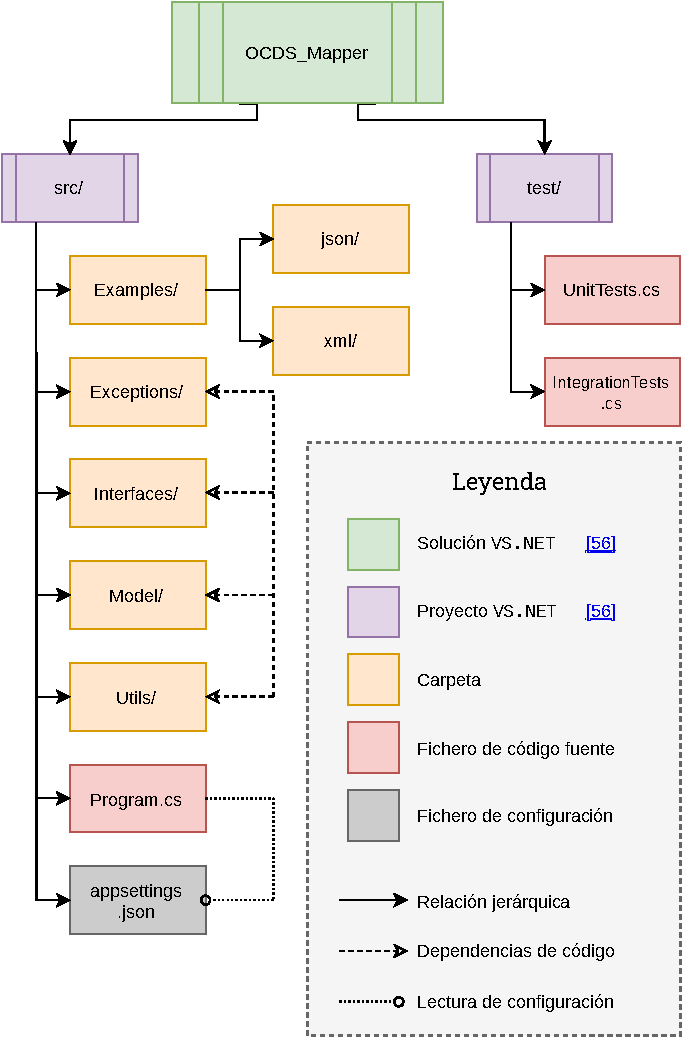
\includegraphics[width=0.65\textwidth]{estructura.pdf}
            \captionof{figure}{Diagrama de estructura de la aplicación}
            \label{fig:estructura}
        \end{figure}
        
    \subsection{Diseño de la arquitectura}
        \subsubsection{Componentes software} \label{subsubsec:componentes}
            Dado que el sistema está diseñado mediante una arquitectura de componentes orientada a servicios, el diseño de la arquitectura se limita a la propia descripción de los componentes que lo integran.
            \\ \\
            Posteriormente, en el \hyperref[subsec:detallado]{diseño detallado del sistema}, se incluirán los diagramas \texttt{UML} individuales de cada componente, acompañados en la sección de \hyperref[subsec:flujo]{flujo de ejecución} por una serie de diagramas de flujo con la representación de la ejecución del sistema.
            \\ \\
            Las interfaces de los componentes del sistema pueden encontrarse en el \hyperref[annex:interfaces]{Anexo I}.
            
            \begin{center}
                \begin{tabular}{|| M{3cm} | M{12cm} ||} 
                    \hline
                        Nombre del componente & Descripción del componente \\
                    \hline\hline
                        \textit{\large Provider} & Componente encargado de la provisión de los datos. Admite cuatro modos de operación: proveer el documento más reciente disponible, proveer un documento específico (ya sea local o en forma de \texttt{URL}), proveer los documentos correspondientes únicamente al día anterior, o proveer un flujo continuo de documentos desde el más reciente hasta no encontrar un fichero enlazado más o abortar la aplicación \\ 
                    \hline
                        \textit{\large Parser} & Componente encargado del parseo de los datos de los documentos de la Plataforma de Contratación Pública. Provee servicios para extraer los espacios de nombres, los elementos dadas sus rutas, etcétera  \\
                    \hline
                        \textit{\large Mapper} & Componente encargado del mapeado de los datos al estándar \texttt{OCDS}. A través de los elementos \texttt{XML} provistos por el \textit{Parser} y las reglas especificadas en \textit{Mappings}, construye el fichero \texttt{JSON} correspondiente al mapeado de cada entrada \texttt{XML} \\
                    \hline
                        \textit{\large Packager} & Componente encargado del empaquetado de los datos ya mapeados. Publica los paquetes de datos de manera local para su posterior carga y procesado a \texttt{RDF} \\
                    \hline
                \end{tabular}
            \end{center}
            \captionof{table}{Tabla de descripción de componentes}
            
            \vspace{0.3cm}
            
            \begin{figure}[h]
                \centering
                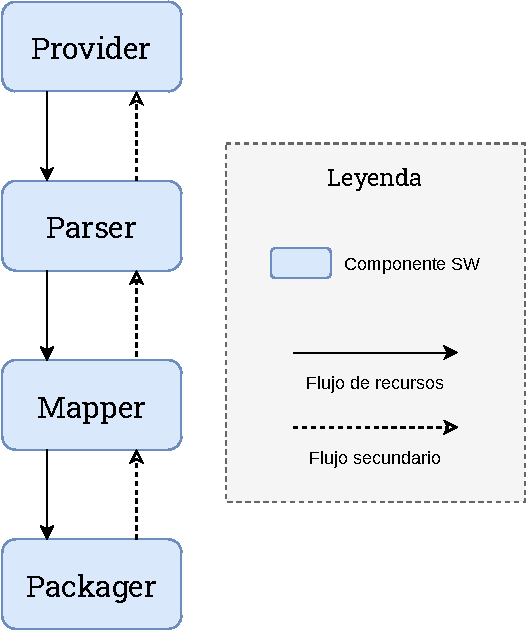
\includegraphics[width=0.5\textwidth]{componentes.pdf}
                \captionof{figure}{Diagrama de los componentes del sistema}
                \label{fig:componentes}
            \end{figure}
            
            En el diagrama de interrelación de componentes (véase \hyperref[fig:componentes]{figura 12}) se pueden apreciar dos tipos de flujo distintos.
\newpage
            El principal, el flujo de recursos, representa el funcionamiento básico del sistema: el componente de provisión de datos (\textit{Provider}) suministra los documentos con los datos de contrataciones públicas bajo el esquema \texttt{CODICE} al componente de extracción de datos (\textit{Parser}). Una vez los datos del documento han sido extraídos, por cada entrada del documento de contrataciones se genera una nueva instancia del componente de mapeado (\textit{Mapper}), que implementa las reglas de mapeado descritas en el componente estático \textit{Mappings}. Cuando el documento ha sido totalmente procesado, el componente de empaquetado de datos (\textit{Packager}) finaliza el pipeline del sistema, publicando los datos de manera local.
            \\ \\
            El flujo secundario representa el uso de métodos entre los distintos componentes, ya sea de manera estática o mediante llamadas a instancias de los componentes.
            
        \subsubsection{Especificación de requisitos}
            Este apartado recoge todos los requisitos, funcionales y de calidad del sistema, que han sido diseñados para la arquitectura del sistema.

            \begin{longtable}{|| M{3cm} | M{12cm} ||} 
                \hline
                    Código del requisito & Descripción del requisito \\
                \hline\hline
                    \texttt{\textit{RF-1}} & El sistema debe ser capaz de descargar documentos de la Plataforma de Contratación Pública \\ 
                \hline
                    \texttt{\textit{RF-2}} & El sistema debe ser capaz de recuperar el documento de licitaciones más reciente \\
                \hline
                    \texttt{\textit{RF-3}} & El sistema debe ser capaz de descargar un documento provisto con una ruta, sea de manera local o remota \\
                \hline
                    \texttt{\textit{RF-4}} & El sistema debe ser capaz de detectar que una ruta a un documento provisto, local o remota, sea incorrecta \\
                \hline
                    \texttt{\textit{RF-5}} & El sistema debe ser capaz de otorgar los documentos provistos de manera asíncrona y bloqueante \\
                \hline
                    \texttt{\textit{RF-6}} & El sistema debe ser capaz de eliminar aquellos documentos que ya hayan sido procesados \\
                \hline
                    \texttt{\textit{RF-7}} & El sistema debe ser capaz de recuperar los espacios de nombres del \texttt{XML} del documento de licitaciones \\
                \hline
                    \texttt{\textit{RF-8}} & El sistema debe ser capaz de proveer los documentos enlazados a los que se están procesando \\
                \hline
                    \texttt{\textit{RF-9}} & El sistema debe ser capaz de recopilar el conjunto de entradas que aparecen en cada documento de licitaciones \\
                \hline
                    \texttt{\textit{RF-10}} & El sistema debe ser capaz de establecer el elemento raíz de cada documento de licitaciones \\
                \hline
                    \texttt{\textit{RF-11}} & El sistema debe ser capaz de detectar que a un documento de licitaciones le falta el elemento raíz \\
                \hline
                    \texttt{\textit{RF-12}} & El sistema debe ser capaz de encontrar un elemento específico en el documento de licitaciones dada su ruta \\
                \hline
                    \texttt{\textit{RF-13}} & El sistema debe ser capaz de encontrar un conjunto de elementos específicos en el documento de licitaciones dada su ruta \\
                \hline
                    Código del requisito & Descripción del requisito \\
                \hline
                \hline
                    \texttt{\textit{RF-14}} & El sistema debe ser capaz de devolver el documento de licitaciones enlazado al que está siendo procesado actualmente \\
                \hline
                    \texttt{\textit{RF-15}} & El sistema debe ser capaz de encontrar un elemento específico a partir de otro en el documento de licitaciones \\
                \hline
                    \texttt{\textit{RF-16}} & El sistema debe ser capaz de devolver el valor de un código descrito en un documento de códigos \\
                \hline
                    \texttt{\textit{RF-17}} & El sistema debe ser capaz de construir un documento en formato \texttt{JSON} con el documento de licitaciones procesado \\
                \hline
                    \texttt{\textit{RF-18}} & El sistema debe ser capaz de detectar una regla de mapeado vacía \\
                \hline
                    \texttt{\textit{RF-19}} & El sistema debe ser capaz de detectar una regla de mapeado de longitud inválida \\
                \hline
                    \texttt{\textit{RF-20}} & El sistema debe ser capaz de detectar una regla de mapeado sin definir \\
                \hline
                    \texttt{\textit{RF-21}} & El sistema debe ser capaz de construir las colecciones de objetos \texttt{JSON} en el documento siendo mapeado \\
                \hline
                    \texttt{\textit{RF-22}} & El sistema debe ser capaz de mapear el elemento \texttt{ContractFolderStatusCode} en el elemento \texttt{tag} \\
                \hline
                    \texttt{\textit{RF-23}} & El sistema debe ser capaz de mapear el eleemnto \texttt{ContractFolderID} en el elemento \texttt{OCID} \\
                \hline
                    \texttt{\textit{RF-24}} & El sistema debe ser capaz de mapear el elemento \texttt{ProcurementProject/Name} en el elemento \texttt{tender.title} \\
                \hline
                    \texttt{\textit{RF-25}} & El sistema debe ser capaz de mapear el elemento \texttt{ProcurementProject/BudgetAmount/
                    EstimatedOverallContractAmount} en el elemento \texttt{tender.value} \\
                \hline
                    \texttt{\textit{RF-26}} & El sistema debe ser capaz de mapear el elemento \texttt{ProcurementProject/BudgetAmount/TotalAmount} en el elemento \texttt{budget.amount} \\
                \hline
                    \texttt{\textit{RF-27}} & El sistema debe ser capaz de mapear el elemento \texttt{ProcurementProject/PlannedPeriod/StartDate} en el elemento \texttt{tender.period.startDate} \\
                \hline
                    \texttt{\textit{RF-28}} & El sistema debe ser capaz de mapear el elemento \texttt{ProcurementProject/PlannedPeriod/EndDate} en el elemento \texttt{tender.period.endDate} \\
                \hline
                    \texttt{\textit{RF-29}} & El sistema debe ser capaz de mapear el elemento \texttt{ProcurementProject/PlannedPeriod/DurationMeasure} en el elemento \texttt{tender.period.durationInDays} \\
                \hline
                    \texttt{\textit{RF-30}} & El sistema debe ser capaz de mapear el elemento \texttt{ProcurementProject/TypeCode} en el elemento \texttt{tender.mainProcurementCategory} \\
                \hline
\newpage
                \hline
                    Código del requisito & Descripción del requisito \\
                \hline
                \hline
                    \texttt{\textit{RF-31}} & El sistema debe ser capaz de mapear el elemento \texttt{ProcurementProjectLot/ID} en los elementos \texttt{tender.lots.id, tender.items\{id, relatedLot\}} \\
                \hline
                    \texttt{\textit{RF-32}} & El sistema debe ser capaz de mapear el elemento \texttt{ProcurementProjectLot/ProcurementProject/BudgetAmount/
                    TotalAmount} en el elemento \texttt{tender.lots.value} \\
                \hline
                    \texttt{\textit{RF-33}} & El sistema debe ser capaz de mapear el elemento \texttt{ProcurementProjectLot/ProcurementProject/
                    RequiredCommodityClassification/ItemClassificationCode} en el elemento \texttt{tender.items.classification} \\
                \hline
                    \texttt{\textit{RF-34}} & El sistema debe ser capaz de mapear el elemento \texttt{TenderingProcess/ProcedureCode} en el elemento \texttt{tender.procurementMethod} \\
                \hline
                    \texttt{\textit{RF-35}} & El sistema debe ser capaz de mapear el elemento \texttt{TenderingProcess/ContractingSystemCode} en el elemento \texttt{tender.procurementMethodDetails\_es} \\
                \hline
                    \texttt{\textit{RF-36}} & El sistema debe ser capaz de mapear el elemento \texttt{TenderingProcess/SubmissionMethodCode} en el elemento \texttt{tender.submissionMethod} \\
                \hline
                    \texttt{\textit{RF-37}} & El sistema debe ser capaz de mapear el elemento \texttt{TenderingTerms/Language/ID} en el elemento \texttt{tender.submissionMethodDetails} \\
                \hline
                    \texttt{\textit{RF-38}} & El sistema debe ser capaz de mapear el elemento \texttt{TenderingProcess/AuctionTerms/AuctionConstraintIndicator} en el elemento \texttt{tender.submissionMethod} \\
                \hline
                    \texttt{\textit{RF-39}} & El sistema debe ser capaz de mapear el elemento \texttt{LocatedContractingParty/Party/PartyName/Name} en el elemento \texttt{parties[i].name} \\
                \hline
                    \texttt{\textit{RF-40}} & El sistema debe ser capaz de mapear el elemento \texttt{LocatedContractingParty/Party/PartyIdentification/ID} en los elementos \texttt{parties[i].\{additionalIdentifiers, id, identifier.\{id, schema\}, roles\}} \\
                \hline
                    \texttt{\textit{RF-41}} & El sistema debe ser capaz de mapear el elemento \texttt{LocatedContractingParty/Party/PostalAddress/Contact} en el elemento \texttt{parties[i].\{address, countryName, contactPoint\}} \\
                \hline
                    \texttt{\textit{RF-42}} & El sistema debe ser capaz de mapear el elemento \texttt{TenderResult/AwardedTenderedProject/ProcurementProjectID} en el elemento \texttt{awards[i].id} \\
                \hline
                    \texttt{\textit{RF-43}} & El sistema debe ser capaz de mapear el elemento \texttt{TenderResult/ResultCode} en el elemento \texttt{awards[i].status} \\
                \hline
\newpage
                \hline
                    Código del requisito & Descripción del requisito \\
                \hline
                \hline
                    \texttt{\textit{RF-44}} & El sistema debe ser capaz de mapear el elemento \texttt{TenderResult/WinningParty} en los elementos \texttt{\{awards[i].suppliers, parties[j]\}} \\
                \hline
                    \texttt{\textit{RF-45}} & El sistema debe ser capaz de mapear el elemento \texttt{TenderResult/AwardedTenderedProject/LegalMonetaryTotal/
                    PayableAmount} en el elemento \texttt{awards[i].value} \\
                \hline
                    \texttt{\textit{RF-46}} & El sistema debe ser capaz de mapear el elemento \texttt{TenderResult/ReceivedTenderQuantity} en el elemento \texttt{tender.numberOfTenderers} \\
                \hline
                    \texttt{\textit{RF-47}} & El sistema debe ser capaz de mapear el elemento \texttt{TenderResult/AwardDate} en el elemento \texttt{awards[i].date} \\
                \hline
                    \texttt{\textit{RF-48}} & El sistema debe ser capaz de mapear el elemento \texttt{TenderResult/Description} en el elemento \texttt{awards[i].description\_es} \\
                \hline
                    \texttt{\textit{RF-49}} & El sistema debe ser capaz de mapear el elemento \texttt{TenderResult/Contract/ID} en el elemento \texttt{contracts[i].id} \\
                \hline
                    \texttt{\textit{RF-50}} & El sistema debe ser capaz de mapear el elemento \texttt{TenderResult/StartDate} en el elemento \texttt{contracts[i].period.startDate} \\
                \hline
                    \texttt{\textit{RF-51}} & El sistema debe ser capaz de detectar las ocurrencias de los identificadores para prevenir los duplicados \\
                \hline
                    \texttt{\textit{RF-52}} & El sistema debe ser capaz de crear un paquete de entrega siguiendo el formato \texttt{OCDS} \\
                \hline
                    \texttt{\textit{RF-53}} & El sistema debe ser capaz de publicar un paquete de entrega de manera local \\
                \hline
                    \texttt{\textit{RF-54}} & El sistema debe ser capaz de detectar argumentos incorrectos \\
                \hline
                    \texttt{\textit{RF-55}} & El sistema debe ser capaz de detectar la falta de argumentos requeridos como el directorio de salida \\
                \hline
            \end{longtable}
            \addtocounter{table}{-1}
            \captionof{table}{Tabla de requisitos funcionales}
            

    
    \subsection{Diseño detallado del sistema} \label{subsec:detallado}
        \subsubsection{Casos de uso del componente de provisión de datos}
    
            \begin{figure}[h]
                \centering
                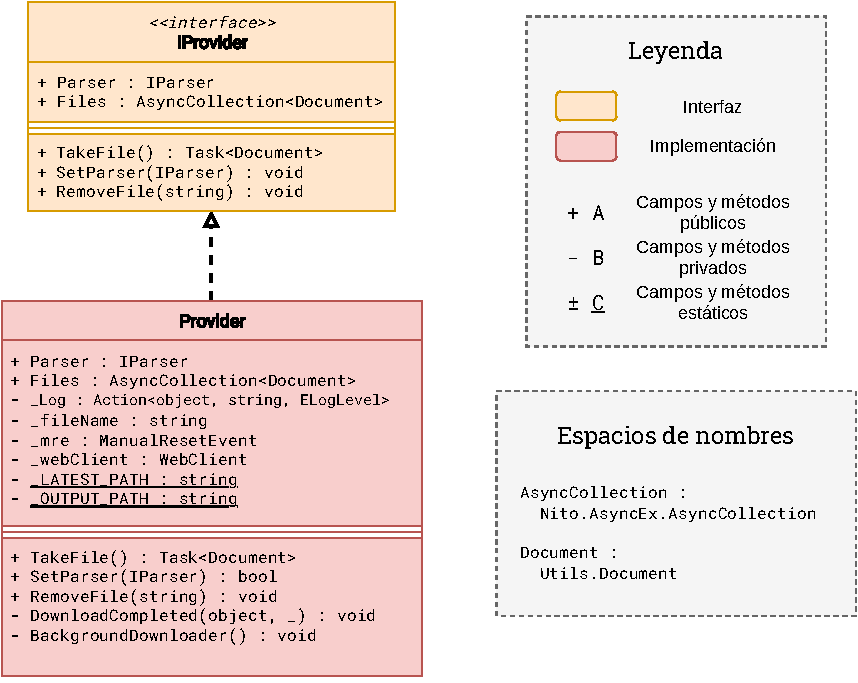
\includegraphics[width=0.8\linewidth]{provider.pdf}
                \captionof{figure}{Diagrama \texttt{UML} del componente \textit{Provider}}
                \label{fig:provider}
            \end{figure}
            
            \paragraph{Caso de uso I: modo de carga local} \mbox{}\\
                El componente de provisión de datos debe ser capaz de cargar en memoria para su posterior procesado un fichero localizado en el sistema de ficheros local de la máquina ejecutando el proceso. También debe notificar si la ruta al fichero local especificado no es correcta o si en ella no existe dicho fichero.
                
            \paragraph{Caso de uso II: modo de descarga remota} \mbox{}\\
                El componente de provisión de datos debe ser capaz de descargar para su posterior procesado un documento de licitaciones desde la Plataforma de Contratación Pública. También debe notificar si la \texttt{URL} no es correcta.
            
            \paragraph{Caso de uso III: provisión simple} \mbox{}\\
                El componente de provisión de datos debe ser, si así se especifica, capaz de proveer un único documento de licitaciones, el cual podrá ser cargado o descargado de manera local o remota, respectivamente. En el caso de una provisión simple de manera remota, el componente tratará de descargar aquel documento más reciente, cuya \texttt{URL} \cite{LICIDIA} queda descrita en el portal de datos abiertos del Ministerio de Hacienda \cite{PORTALHAC}.
                
            \paragraph{Caso de uso IV: provisión continua} \mbox{}\\
                El componente de provisión de datos debe ser capaz, si así se especifica, y sólo en el modo de descarga remota, de encontrar en el documento de licitaciones siendo descargado el enlace al siguiente documento, con el fin de proveer un flujo continuo de recursos para el procesado en el sistema. El primer documento del flujo será el más reciente, descrito en el apartado anterior.
                
            \paragraph{Caso de uso V: provisión diaria} \mbox{}\\
                El componente de provisión de datos debe ser capaz, si así se especifica, y sólo en el modo de descarga remota, de igual manera que con el caso de uso de la provisión continua, de proveer un flujo de recursos para ser procesados, con la salvedad que dicho flujo se limite exclusivamente al conjunto de documentos publicados en el día anterior.
                
        \subsubsection{Casos de uso del componente de parseo de datos}
    
            \begin{figure}[h]
                \centering
                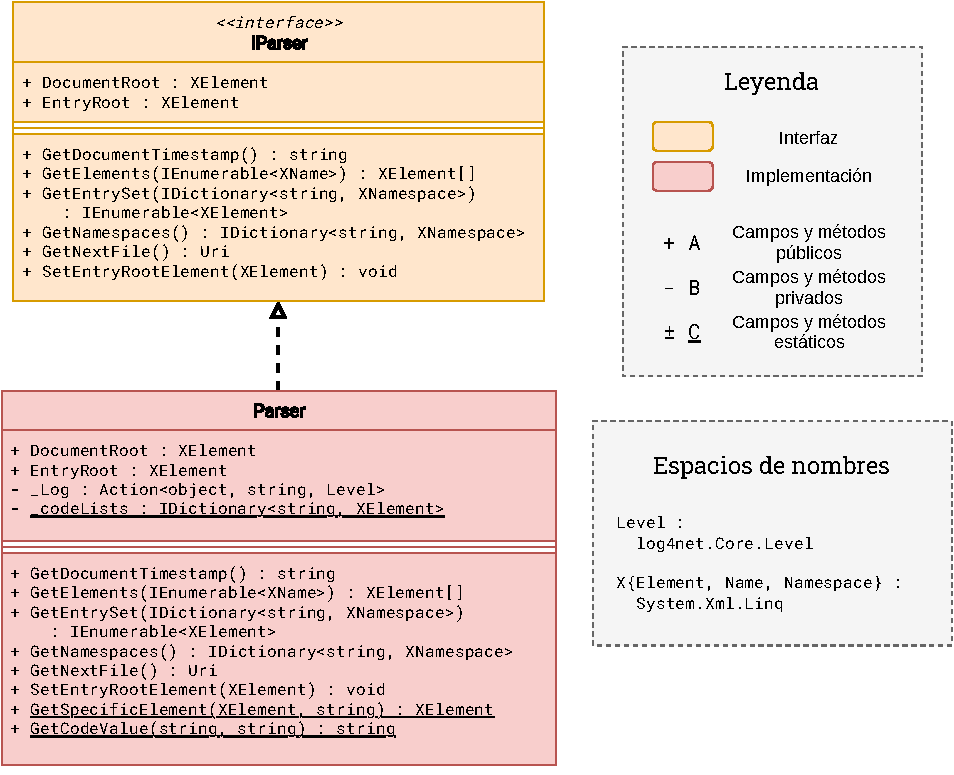
\includegraphics[]{parser.pdf}
                \captionof{figure}{Diagrama \texttt{UML} del componente \textit{Parser}}
                \label{fig:parser}
            \end{figure}
            
            \paragraph{Caso de uso I: extracción de elementos} \mbox{}\\
                El componente de parseo de datos debe ser capaz de extraer todos los elementos requeridos dado un documento de licitaciones. Los elementos de interés para ser extraídos son, entre otros, el \textit{timestamp} de la publicación, el conjunto de entradas, el conjunto de espacios de nombres, o la ruta al documento enlazado.
                
            \paragraph{Caso de uso II: extracción específica de elementos} \mbox{}\\
                El componente de parseo de datos debe ser capaz de, dada una ruta que iterar o un punto del que partir, bajar por los niveles del documento y extraer un elemento específico, con el objetivo de realizar posteriores mapeados lo más independientes posible.
            
            \paragraph{Caso de uso III: obtención de códigos} \mbox{}\\
                El componente de parseo de datos debe ser capaz de descargar en memoria aquellos documentos de códigos usados por el sistema y poder extraer de ellos los valores necesitados en cada momento.
\newpage
        \subsubsection{Casos de uso del componente de mapeado de datos}
    
            \begin{figure}[h]
                \centering
                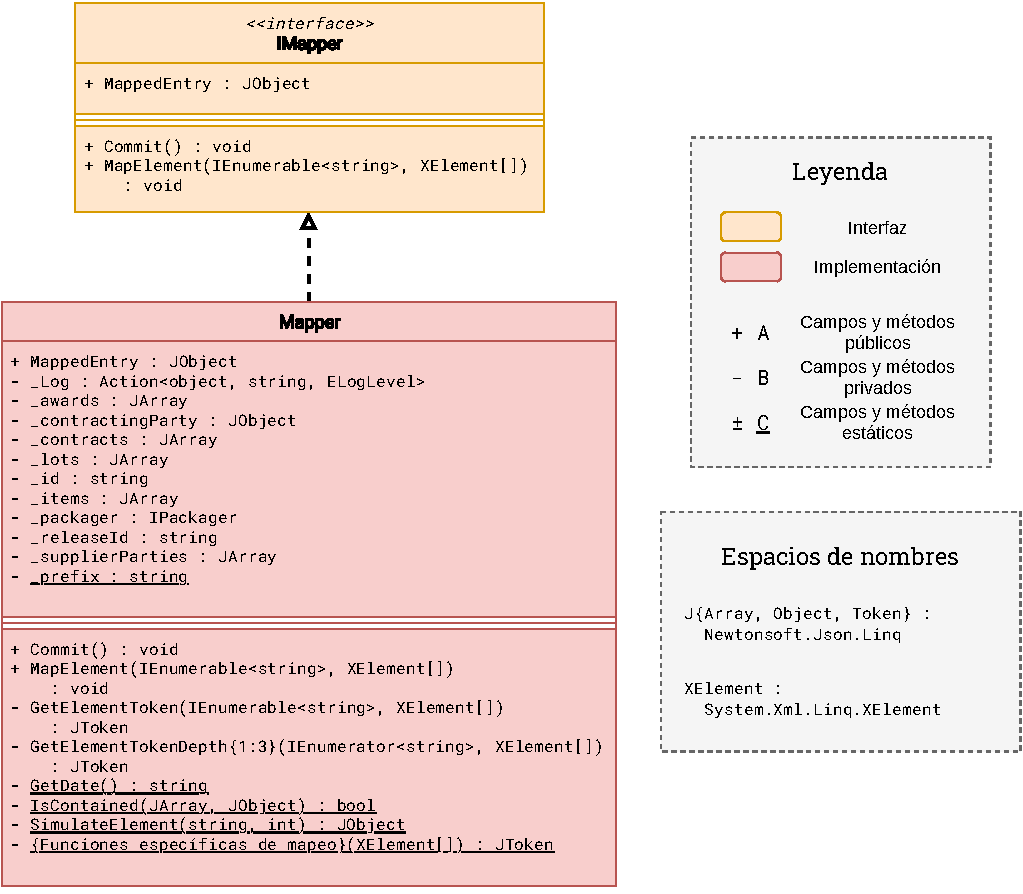
\includegraphics[]{mapper.pdf}
                \captionof{figure}{Diagrama \texttt{UML} del componente \textit{Mapper}}
                \label{fig:mapper}
            \end{figure}
            
            \paragraph{Caso de uso I: mapeado unitario de elementos} \mbox{}\\
                El componente de mapeado de datos debe ser capaz de realizar mapeados unitarios de elementos extraídos de los documentos de licitaciones (esquema \texttt{CODICE}) al esquema \texttt{OCDS}. Para ello, al componente se le indicará tanto el elemento a procesar como la ruta en la que debe almacenar el resultado.
                
            \paragraph{Caso de uso II: mapeado múltiple de elementos} \mbox{}\\
                El componente de mapeado de datos debe ser capaz de realizar mapeados múltiples de elementos siempre y cuando no pueda realizar mapeados unitarios de dichos elementos. Para ello, al componente se le proveera un conjunto de elementos emparentados de la forma más próxima posible. Cuando finalice la ejecución del mapeado, el componente deberá persistir las estructuras de datos en el objeto final para su posterior empaquetado.
                
\newpage
        \subsubsection{Casos de uso del componente de empaquetado de datos}
    
            \begin{figure}[h]
                \centering
                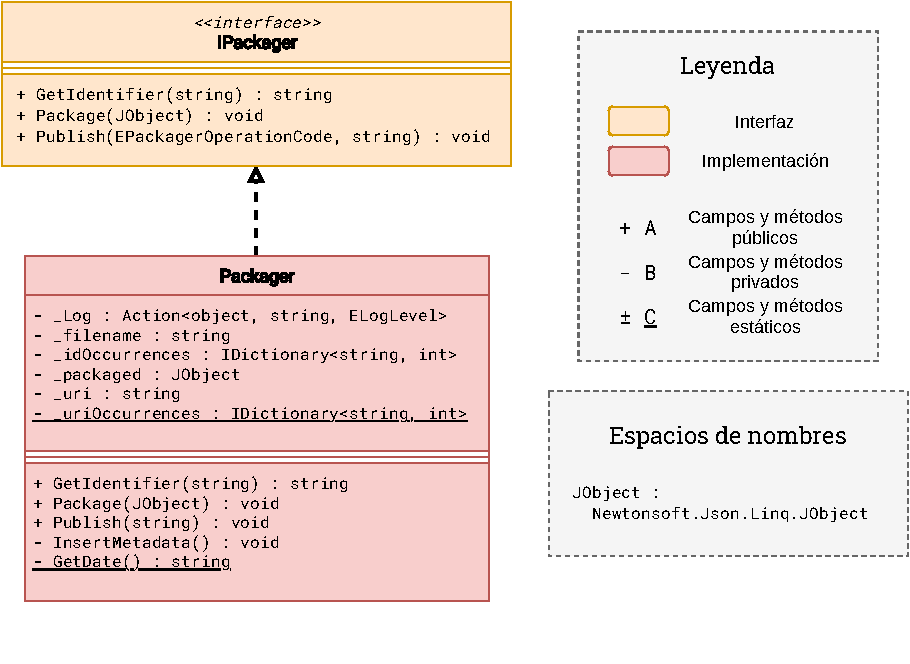
\includegraphics[]{packager.pdf}
                \captionof{figure}{Diagrama \texttt{UML} del componente \textit{Packager}}
                \label{fig:packager}
            \end{figure}
            
            \paragraph{Caso de uso I: empaquetado} \mbox{}\\
                El componente de empaquetado de datos debe ser capaz de recopilar las entradas de los documentos procesados que le lleguen por parte de otros componentes del sistema para persistirlos en un fichero de manera local.
                
            \paragraph{Caso de uso II: evitar colisiones} \mbox{}\\
                El componente de empaquetado de datos debe ser capaz de almacenar temporalmente los identificadores tanto de los propios documentos de licitaciones como de elementos concretos de cada entrada para así evitar colisiones de identificadores no únicos.
        
    \subsection{Trazabilidad de requisitos} \label{subsec:trazabilidad}
        \begin{longtable}{|| M{3cm} | M{12cm} ||} 
                \hline
                    Código del requisito & Ruta del elemento de prueba \\
                \hline\hline
                    \texttt{\textit{RF-1}} & \texttt{UnitTests.ProviderTests.\textit{TestConstructor\{1:4\}}} \\ 
                \hline
                    \texttt{\textit{RF-2}} & \texttt{UnitTests.ProviderTests.\textit{TestConstructor1}} \\
                \hline
                    \texttt{\textit{RF-3}} & \texttt{UnitTests.ProviderTests.\textit{TestConstructor\{2:3\}}} \\
                \hline
                    \texttt{\textit{RF-4}} & \texttt{UnitTests.ProviderTests.\textit{TestConstructor4}} \\
                \hline
                    Código del requisito & Ruta del elemento de prueba \\
                \hline
                \hline
                    \texttt{\textit{RF-5}} & \texttt{UnitTests.ProviderTests.\textit{TestTakeFile\{1:2\}}} \\
                \hline
                    \texttt{\textit{RF-6}} & \texttt{UnitTests.ProviderTests.\textit{TestRemoveFile\{1:2\}}} \\
                \hline
                    \texttt{\textit{RF-7}} & \texttt{UnitTests.ParserTests.\textit{TestGetNamespaces}} \\
                \hline
                    \texttt{\textit{RF-8}} & \texttt{IntegrationTests.\textit{TestProviderParser}} \\
                \hline
                    \texttt{\textit{RF-9}} & \texttt{IntegrationTests.ParserTests.\textit{TestGetEntrySet}} \\
                \hline
                    \texttt{\textit{RF-10}} & \texttt{IntegrationTests.ParserTests.\textit{TestSetEntryRootElement1}} \\
                \hline
                    \texttt{\textit{RF-11}} & \texttt{IntegrationTests.ParserTests.\textit{TestSetEntryRootElement2}} \\
                \hline
                    \texttt{\textit{RF-12}} & \texttt{IntegrationTests.ParserTests.\textit{TestGetElements1}} \\
                \hline
                    \texttt{\textit{RF-13}} & \texttt{IntegrationTests.ParserTests.\textit{TestGetElements2}} \\
                \hline
                    \texttt{\textit{RF-14}} & \texttt{UnitTests.ParserTests.\textit{TestGetNextFile\{1:2\}}} \\
                \hline
                    \texttt{\textit{RF-15}} & \texttt{IntegrationTests.ParserTests.\textit{TestGetSpecificElement}} \\
                \hline
                    \texttt{\textit{RF-16}} & \texttt{UnitTests.ParserTests.\textit{TestGetCodeValue}} \\
                \hline
                    \texttt{\textit{RF-17}} & \texttt{UnitTests.MapperTests.\textit{TestConstructor}} \\
                \hline
                    \texttt{\textit{RF-18}} & \texttt{UnitTests.MapperTests.\textit{TestMapElement1}} \\
                \hline
                    \texttt{\textit{RF-19}} & \texttt{UnitTests.MapperTests.\textit{TestMapElement2}} \\
                \hline
                    \texttt{\textit{RF-20}} & \texttt{UnitTests.MapperTests.\textit{TestMapElement3}} \\
                \hline
                    \texttt{\textit{RF-21}} & \texttt{IntegrationTests.MapperTests.\textit{TestCommit}} \\
                \hline
                    \texttt{\textit{RF-22}} & \texttt{UnitTests.MapperTests.\textit{TagTests}} \\
                \hline
                    \texttt{\textit{RF-23}} & \texttt{UnitTests.MapperTests.\textit{OCIDTests}} \\
                \hline
                    \texttt{\textit{RF-24}} & \texttt{UnitTests.MapperTests.\textit{TenderTitleTests}} \\
                \hline
                    \texttt{\textit{RF-25}} & \texttt{UnitTests.MapperTests.\textit{TenderValueTests}} \\
                \hline
                    \texttt{\textit{RF-26}} & \texttt{UnitTests.MapperTests.\textit{BudgetAmountTests}} \\
                \hline
                    \texttt{\textit{RF-27}} & \texttt{UnitTests.MapperTests.\textit{TenderPeriodStartDateTests}} \\
                \hline
                    \texttt{\textit{RF-28}} & \texttt{UnitTests.MapperTests.\textit{TenderPeriodEndDateTests}} \\
                \hline
                    \texttt{\textit{RF-29}} & \texttt{UnitTests.MapperTests.\textit{TenderPeriodDurationInDaysTests}} \\
                \hline
                    \texttt{\textit{RF-30}} & \texttt{UnitTests.MapperTests.\textit{TenderMainProcurementCategoryTests}} \\
                \hline
                    \texttt{\textit{RF-31}} & \texttt{UnitTests.MapperTests.\textit{TenderLotsIdTests}} \\
                \hline
                    \texttt{\textit{RF-32}} & \texttt{UnitTests.MapperTests.\textit{TenderLotsValueTests}} \\
                \hline
                    \texttt{\textit{RF-33}} & \texttt{UnitTests.MapperTests.\textit{TenderItemsClassificationTests}} \\
                \hline
                    \texttt{\textit{RF-34}} & \texttt{UnitTests.MapperTests.\textit{TenderProcurementMethodTests}} \\
                \hline
                    \texttt{\textit{RF-35}} & \texttt{UnitTests.MapperTests.\textit{TenderProcurementMethodDetailsTests}} \\
                \hline
                    \texttt{\textit{RF-36}} & \texttt{UnitTests.MapperTests.\textit{TenderSubmissionMethodTests}} \\
                \hline
                    \texttt{\textit{RF-37}} & \texttt{UnitTests.MapperTests.\textit{TenderSubmissionMethodDetailsTests}} \\
                \hline
                    \texttt{\textit{RF-38}} & \texttt{UnitTests.MapperTests.\textit{TenderSubmissionMethodTests}} \\
                \hline
                \hline
                    Código del requisito & Ruta del elemento de prueba \\
                \hline
                    \texttt{\textit{RF-39}} & \texttt{UnitTests.MapperTests.\textit{PartiesNameTests}} \\
                \hline
                    \texttt{\textit{RF-40}} & \texttt{UnitTests.MapperTests.\textit{PartiesIdentifierTests}} \\
                \hline
                    \texttt{\textit{RF-41}} & \texttt{UnitTests.MapperTests.\textit{PartiesFieldsTests}} \\
                \hline
                    \texttt{\textit{RF-42}} & \texttt{UnitTests.MapperTests.\textit{AwardIdTests}} \\
                \hline
                    \texttt{\textit{RF-43}} & \texttt{UnitTests.MapperTests.\textit{AwardStatusTests}} \\
                \hline
                    \texttt{\textit{RF-44}} & \texttt{UnitTests.MapperTests.\textit{AwardSupplierTests}} \\
                \hline
                    \texttt{\textit{RF-45}} & \texttt{UnitTests.MapperTests.\textit{AwardValueTests}} \\
                \hline
                    \texttt{\textit{RF-46}} & \texttt{UnitTests.MapperTests.\textit{TenderNumberOfTenderersTests}} \\
                \hline
                    \texttt{\textit{RF-47}} & \texttt{UnitTests.MapperTests.\textit{AwardDateTests}} \\
                \hline
                    \texttt{\textit{RF-48}} & \texttt{UnitTests.MapperTests.\textit{AwardDescriptionTests}} \\
                \hline
                    \texttt{\textit{RF-49}} & \texttt{UnitTests.MapperTests.\textit{ContractIdTests}} \\
                \hline
                    \texttt{\textit{RF-50}} & \texttt{UnitTests.MapperTests.\textit{ContractPeriodStartDateTests}} \\
                \hline
                    \texttt{\textit{RF-51}} & \texttt{UnitTests.PackagerTests.\textit{TestGetIdentifier}} \\
                \hline
                    \texttt{\textit{RF-52}} & \texttt{UnitTests.PackagerTests.\textit{TestPackage}} \\
                \hline
                    \texttt{\textit{RF-53}} & \texttt{UnitTests.PackagerTests.\textit{TestPublish}} \\
                \hline
                    \texttt{\textit{RF-54}} & \texttt{IntegrationTests.ProgramTests.\textit{TestProgram\{1:3\}}} \\
                \hline
                    \texttt{\textit{RF-55}} & \texttt{IntegrationTests.ProgramTests.\textit{TestProgram4}} \\
                \hline
        \end{longtable}
        \addtocounter{table}{-1}
        \captionof{table}{Tabla de trazabilidad de requisitos}
        
    \vspace{1cm}
    
    \subsection{Flujo de ejecución} \label{subsec:flujo}
        
        \begin{figure}[!htb]
            \centering
            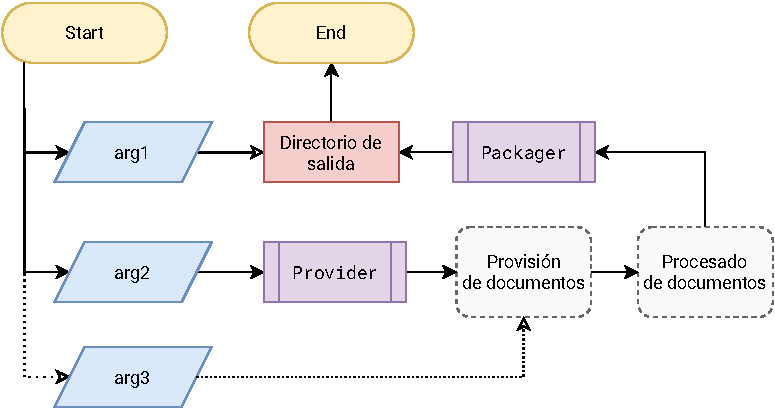
\includegraphics[width=0.825\textwidth]{main_flow.pdf}
            \captionof{figure}{Flujo de ejecución general de la aplicación}
            \label{fig:mainflow}
        \end{figure}
        
        \noindent En la \hyperref[fig:mainflow]{figura 17} se puede apreciar la representación del flujo principal de la aplicación \textit{OCDS\_Mapper}. En primer lugar, cabe destacar la presencia de dos argumentos obligatorios, siendo el primero la ruta del directorio de salida de los ficheros que se generen, y el segundo el descriptor del modo de operación que se pretende ejecutar.
        \\ \\
        En las dos siguientes figuras se detallan los flujos de ejecución correspondientes a la provisión y al procesado de documentos, con el objetivo de simplificar y hacer más clara la representación del funcionamiento del programa.
        
        \begin{figure}[!htb]
            \centering
            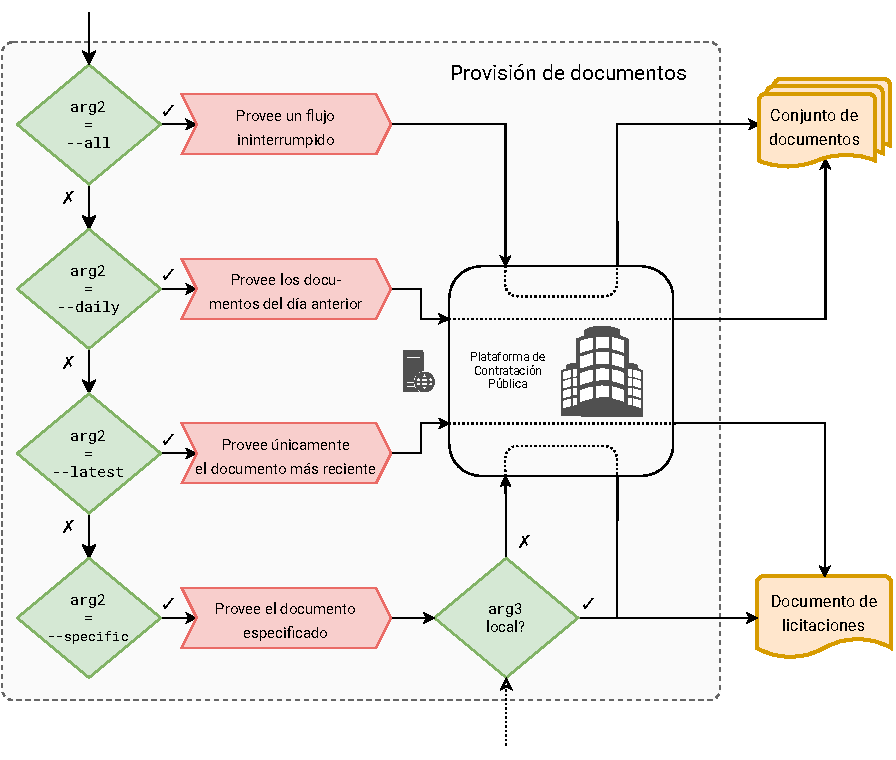
\includegraphics[width=\textwidth]{provider_flow.pdf}
            \captionof{figure}{Flujo de ejecución de la provisión de documentos}
            \label{fig:providerflow}
        \end{figure}
        
        \noindent Mediante la representación del flujo de provisión de documentos se se pueden apreciar los distintos modos de operación del sistema, detallados en secciones previas. Los modos \texttt{--all} y \texttt{--daily} proveen un conjunto de documentos, mientras que los otros dos modos, \texttt{--latest} y \texttt{--specific} proveen un único documento.
        \\ \\
        Este último modo, además, es el único que no accede a la Plataforma de Contratación Pública para descargar documentos si la ruta provista coincide con un archivo local.
        
    \vspace{3cm}
        
        \begin{figure}[!htb]
            \centering
            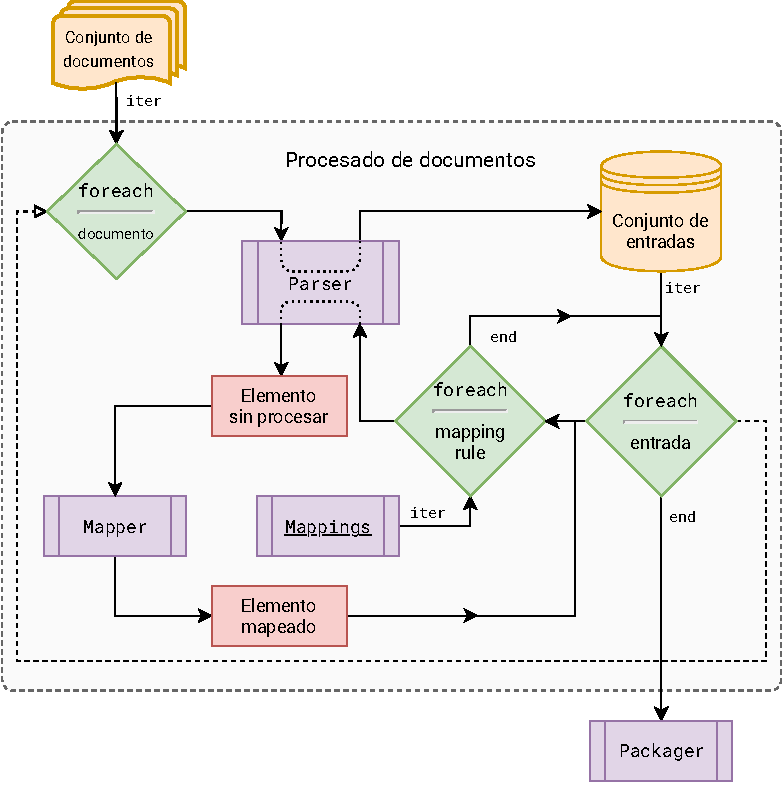
\includegraphics[width=0.95\textwidth]{process_flow.pdf}
            \captionof{figure}{Flujo de ejecución del procesado de documentos}
            \label{fig:processflow}
        \end{figure}
        
        \noindent Para la representación del flujo de procesado de documentos se ha utilizado como \textit{input} un conjunto de documentos en vez de uno único, dado que éste es el caso general y los modos que proveen un solo documento son un caso particular, siendo el conjunto de longitud 1.
        \\ \\
        Por cada documento de licitaciones, se inicializa un componente de parseo que extrae el conjunto de entradas. El procesamiento se realiza entrada a entrada, y en cada una de ellas se evalúan las reglas de mapeado descritas en la clase estática \textit{Mappings}. Se solicita al componente \textit{Parser} que devuelva el elemento concreto de la entrada descrito por la regla de mapeado siendo evaluada, y es el componente \textit{Mapper} el que realiza la transformación de la información de \texttt{CODICE} a \texttt{OCDS}.
        \\ \\
        Una vez cada documento ha sido completamente procesado al finalizar de iterar el conjunto de entradas del mismo, se llama al componente de empaquetado para persistir el documento mapeado.
        
\newpage
    \subsection{Cobertura de código}
        Con el objetivo de proveer un software de calidad, el sistema desarrollado ha sido analizado mediante la plataforma \textit{SonarQube} \cite{SONARQUBE}, capaz de realizar una evaluación del código fuente de manera estática para obtener métricas que sirvan para mejorar la calidad y la seguridad del sistema siendo desarrollado.
        \\ \\
        
        \begin{figure}[h]
            \centering
            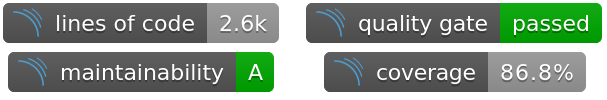
\includegraphics[width=0.625\textwidth]{sonarqube_metrics.png}
            \captionof{figure}{Métricas registradas por \textit{SonarQube}}
            \label{fig:sonarmetrics}
        \end{figure}
        
        \noindent Mediante todos los \textit{tests} descritos en la sección de \hyperref[subsec:trazabilidad]{trazabilidad de requisitos} se ha conseguido una cobertura del código del 86.8\%, sobre las más de 2600 líneas de código de la aplicación. De acuerdo a la \textit{quality gate} por defecto de \textit{SonarQube} para el lenguaje \texttt{C\#}, dicha métrica de cobertura de código es superior al límite (80\%).
        \\ \\
        Entre otras condiciones que se han superado para superar dichas condiciones mínimas, se encuentran la de la duplicidad de líneas (0\%, el límite es 3\%), y los \textit{ratings} de mantenibilidad, fiabilidad y seguridad en calificación \texttt{A}.
        \\ \\
        Se han realizado algunas excepciones al análisis estático del código, cuyas justificaciones se presentan a continuación:
        \begin{itemize}
            \item Regla \texttt{S125}: \textit{"Sections of code should not be commented out"} \cite{SONAR125}. Ignorada debido a que se generaba la alerta en comentarios informativos del funcionamiento de los métodos.
            \item Regla \texttt{S1168}: \textit{"Empty arrays and collections should be returned instead of null"} \cite{SONAR1168}. Ignorada debido a que teniendo el cuenta la implementación del componente \textit{Mapper}, los métodos que no devuelven un objeto \texttt{JObject} devuelven \texttt{null} debido a que el objeto \texttt{JObject} vacío representa un elemento \texttt{JSON} vacío, lo cual no es equivalente a \texttt{null}.
            \item Regla \texttt{S3776}: \textit{"Cognitive Complexity of functions should not be too high"} \cite{SONAR3776}. Por el motivo descrito en el apartado anterior, debido a que cada regla de mapeado está implementada en un sólo método por motivos del modelado del sistema, se ha ignorado esta regla en dichos métodos.
        \end{itemize}
    
\newpage
    \section{Correspondencias entre \texttt{CODICE} y \texttt{OCDS}}

    En esta sección se describirán las correspondencias que se han establecido entre los elementos del estándar \texttt{CODICE} y el estándar \texttt{OCDS}. Dichas correspondencias han sido las implementadas en el \hyperref[sec:software]{software desarrollado}.
    \\ \\
    No todos los elementos de \texttt{CODICE} han sido mapeados, ni todos los campos de \texttt{OCDS} han sido cubiertos, pero sí se han considerado aquellos elementos de mayor interés. Una lista exhaustiva sobre el estado de los elementos puede encontrarse en la siguiente hoja de cálculo \cite{CHECKLIST}.

    \vspace{0.3cm}
    
    \subsection{Datos generales del expediente}
    
    Elementos correspondientes a información genérica del expediente de licitaciones.
    
        \subsubsection{Estado}
            \begin{itemize}
                \item \textbf{Elemento en el esquema \texttt{CODICE}}:
                    \tabto{7.6cm} \texttt{cac-place-ext:ContractFolderStatus/} \\
                    \tabto{7.6cm} \texttt{\textit{cbc-place-ext:ContractFolderStatusCode}}
                \item \textbf{Elemento en el esquema \texttt{OCDS}}:
                    \tabto{7.6cm} \texttt{\textit{tag}}
                \item \textbf{Comentarios}: La lista de posibles códigos del elemento en \texttt{CODICE} se encuentra en el siguiente enlace \cite{CR1}.
                    La lista análoga de códigos en el esquema \texttt{OCDS} se puede consultar en el siguiente enlace \cite{CR2}.
                    La correspondencia entre ambas listas de códigos se ha establecido de la siguiente manera:
                        \subitem - \texttt{PRE} (Anuncio previo) $\rightarrow$ \texttt{planning}
                        \subitem - \texttt{PUB} (En plazo) $\rightarrow$ \texttt{tender}
                        \subitem - \texttt{EV} (Pendiente de adjudicación) $\rightarrow$ \texttt{tender}
                        \subitem - \texttt{ADJ} (Adjudicada) $\rightarrow$ \texttt{award}
                        \subitem - \texttt{RES} (Resuelta) $\rightarrow$ \texttt{contract}
                        \subitem - \texttt{ANUL} (Anulada) $\rightarrow$ \texttt{awardCancellation}
            \end{itemize}
        
        \subsubsection{Número de expediente}
            \begin{itemize}
                \item \textbf{Elemento en el esquema \texttt{CODICE}}:
                    \tabto{7.6cm} \texttt{cac-place-ext:ContractFolderStatus/} \\
                    \tabto{7.6cm} \texttt{\textit{cbc:ContractFolderID}}
                \item \textbf{Elemento en el esquema \texttt{OCDS}}:
                    \tabto{7.6cm} \texttt{\textit{ocid}}
                \item \textbf{Comentarios}: En el esquema de \texttt{OCDS}, los procesos de contratación deben identificarse mediante un código unívoco que será idéntico en cualquier posterior entrega del mismo proceso de contratación. Para asegurar que dichos códigos no puedan colisionar, \texttt{OCDS} provee a los publicadores prefijos que concatenar a los identificadores internos para así asegurar la creación de identificadores globales únicos.
            \end{itemize}
        
        \subsubsection{Objeto del contrato}
            \begin{itemize}
                \item \textbf{Elemento en el esquema \texttt{CODICE}}:
                    \tabto{7.6cm} \texttt{cac-place-ext:ContractFolderStatus/} \\
                    \tabto{7.6cm} \texttt{cac:ProcurementProject/} \\
                    \tabto{7.6cm} \texttt{\textit{cbc:Name}}
                \item \textbf{Elemento en el esquema \texttt{OCDS}}:
                    \tabto{7.6cm} \texttt{tender.\textit{title}}
            \end{itemize}
        
        \subsubsection{Valor estimado e importe de licitación}
            \begin{itemize}
                \item \textbf{Elementos en el esquema \texttt{CODICE}}:
                    \tabto{7.7cm} \texttt{cac-place-ext:ContractFolderStatus/} \\
                    \tabto{7.7cm} \texttt{cac:ProcurementProject/} \\
                    \tabto{7.7cm} \texttt{cac:BudgetAmount/} \\
                    \tabto{7.7cm} \{\texttt{\textit{cbc:EstimatedOverallContractAmount}}, \\
                    \tabto{7.7cm} \texttt{\textit{cbc:TotalAmount}}\}
                \item \textbf{Elementos en el esquema \texttt{OCDS}}:
                    \tabto{7.7cm} \texttt{EstimatedOverallContractAmount} \\ \tabto{8cm} $\rightarrow$ \texttt{tender.\textit{value}} \\
                    \tabto{7.7cm} \texttt{TotalAmount} \\ \tabto{8cm} $\rightarrow$ \texttt{planning.budget.\textit{amount}}
            \end{itemize}
        
        \subsubsection{Duración del contrato}
            \begin{itemize}
                \item \textbf{Elementos en el esquema \texttt{CODICE}}:
                    \tabto{7.7cm} \texttt{cac-place-ext:ContractFolderStatus/} \\
                    \tabto{7.7cm} \texttt{cac:ProcurementProject/} \\
                    \tabto{7.7cm} \texttt{cac:PlannedPeriod/} \\
                    \tabto{7.7cm} \{\texttt{\textit{cbc:StartDate}}, \\
                    \tabto{7.7cm} \{\texttt{\textit{cbc:EndDate}}, \\
                    \tabto{7.7cm} \texttt{\textit{cbc:DurationMeasure}}\}\}
                \item \textbf{Elementos en el esquema \texttt{OCDS}}:
                    \tabto{7.7cm} \texttt{StartDate} \\ \tabto{8cm} $\rightarrow$ \texttt{tender.tenderPeriod.\textit{startDate}} \\
                    \tabto{7.7cm} \texttt{EndDate} \\ \tabto{8cm} $\rightarrow$ \texttt{tender.tenderPeriod.\textit{endDate}}
                    \tabto{7.7cm} \texttt{DurationMeasure} \\ \tabto{8cm} $\rightarrow$ \texttt{tender.tenderPeriod.\textit{durationInDays}}
                \item \textbf{Comentarios}: La duración prevista del contrato puede expresarse mediante una fecha de inicio y una de final, o bien mediante una fecha de inicio y una duración prevista, cuyos valores pueden ser expresados mediante días (\texttt{DAY}), meses (\texttt{MON}) o años (\texttt{ANN}).
            \end{itemize}
        
        \subsubsection{Tipo de contrato}
            \begin{itemize}
                \item \textbf{Elemento en el esquema \texttt{CODICE}}:
                    \tabto{7.6cm} \texttt{cac-place-ext:ContractFolderStatus/} \\
                    \tabto{7.6cm} \texttt{cac:ProcurementProject/} \\
                    \tabto{7.6cm} \texttt{\textit{cbc:TypeCode}}
                \item \textbf{Elemento en el esquema \texttt{OCDS}}:
                    \tabto{7.6cm} \texttt{tender.\textit{mainProcurementCategory}}
                \item \textbf{Comentarios}: La lista de posibles valores que pueden tomar los códigos que describen los tipos de contrato en \texttt{CODICE} pueden encontrarse en el siguiente enlace \cite{CR3}. La lista análoga de códigos en el esquema \texttt{OCDS} se puede consultar en el siguiente enlace \cite{CR4}. La correspondencia entre ambas listas de códigos se ha establecido de la siguiente manera:
                        \subitem - \texttt{1} (Suministros) $\rightarrow$ \texttt{goods}
                        \subitem - \texttt{2} (Servicios) $\rightarrow$ \texttt{services}
                        \subitem - \texttt{3} (Obras) $\rightarrow$ \texttt{works}
                        \subitem - \texttt{21} (Gestión de servicios públicos) $\rightarrow$ \texttt{services}
                        \subitem - \texttt{22} (Gestión de servicios) $\rightarrow$ \texttt{services}
                        \subitem - \texttt{31} (Concesión de obras públicas) $\rightarrow$ \texttt{works}
                        \subitem - \texttt{32} (Concesión de obras) $\rightarrow$ \texttt{works}
            \end{itemize}
        
        \subsubsection{Enlaces de descarga de pliegos}
            \begin{itemize}
                \item \textbf{Elementos en el esquema \texttt{CODICE}}:
                    \tabto{7.7cm} \texttt{cac-place-ext:ContractFolderStatus/} \\
                    \tabto{7.7cm} \{\texttt{cac:LegalDocumentReference/}, \\
                    \tabto{7.7cm} \texttt{cac:TechnicalDocumentReference/}, \\
                    \tabto{7.7cm} \texttt{cac:AdditionalDocumentReference/}\} \\
                    \tabto{7.7cm} \texttt{\textit{cbc:ID}},\\
                    \tabto{7.7cm} \texttt{cac:Attachment/} \\
                    \tabto{7.7cm} \texttt{cac:ExternalReference/} \\
                    \tabto{7.7cm} \texttt{\textit{cbc:URI}}
                \item \textbf{Elemento en el esquema \texttt{OCDS}}:
                    \tabto{7.7cm} \texttt{tender.\textit{documents}}
                \item \textbf{Comentarios}: Los distintos pliegos que pueden documentar un proceso de contratación vienen descritos, en su tipo, por el elemento inmediatamente inferior a \texttt{ContractFolderStatus}, y su mapeo al esquema \texttt{OCDS} se representa mediante la lista de códigos documentType \cite{CR5}.
                        \subitem - LegalDocumentReference $\rightarrow$ \texttt{?}
                        \subitem - TechnicalDocumentReference $\rightarrow$ \texttt{technicalSpecifications}
                        \subitem - AdditionalDocumentReference $\rightarrow$ \texttt{?}
            \end{itemize}

    \vspace{0.3cm}
    
    \subsection{Lotes}
        
        El uso de lotes en el esquema \texttt{OCDS} viene otorgado por la extensión de mismo nombre \cite{CR6}.
    
        \subsubsection{Número de lote}
            \begin{itemize}
                \item \textbf{Elemento en el esquema \texttt{CODICE}}:
                    \tabto{7.6cm} \texttt{cac-place-ext:ContractFolderStatus/} \\
                    \tabto{7.6cm} \texttt{cac:ProcurementProjectLot/} \\
                    \tabto{7.6cm} \texttt{\textit{cbc:ID}}
                \item \textbf{Elementos en el esquema \texttt{OCDS}}:
                    \tabto{7.6cm} \texttt{tender.lots[i].\textit{id}} \\
                    \tabto{7.6cm} \texttt{tender.items[i].\textit{id}} \\
                    \tabto{7.6cm} \texttt{tender.items[i].\textit{relatedLot}} \\
                \item \textbf{Comentarios}: En todos los apartados de esta sección se utilizará la notación \texttt{lots[i]} e \texttt{items[i]} para referirse a los i-ésimos objetos representando el lote y el artículo, respectivamente, dentro de las colecciones de éstos. El campo \texttt{relatedLot} se utilizará para enlazar el artículo con su lote.
            \end{itemize}
            
        \subsubsection{Objeto del lote}
            \begin{itemize}
                \item \textbf{Elemento en el esquema \texttt{CODICE}}:
                    \tabto{7.6cm} \texttt{cac-place-ext:ContractFolderStatus/} \\
                    \tabto{7.6cm} \texttt{cac:ProcurementProjectLot/} \\
                    \tabto{7.6cm} \texttt{cac:ProcurementProject/} \\
                    \tabto{7.6cm} \texttt{\textit{cbc:Name}}
                \item \textbf{Elemento en el esquema \texttt{OCDS}}:
                    \tabto{7.6cm} \texttt{tender.lots[i].\textit{name}}
            \end{itemize}
        
        \subsubsection{Importe del lote}
            \begin{itemize}
                \item \textbf{Elemento en el esquema \texttt{CODICE}}:
                    \tabto{7.6cm} \texttt{cac-place-ext:ContractFolderStatus/} \\
                    \tabto{7.6cm} \texttt{cac:ProcurementProjectLot/} \\
                    \tabto{7.6cm} \texttt{cac:ProcurementProject/} \\
                    \tabto{7.6cm} \texttt{cac:BudgetAmount/} \\
                    \tabto{7.6cm} \texttt{\textit{cbc:TotalAmount}}
                \item \textbf{Elemento en el esquema \texttt{OCDS}}:
                    \tabto{7.6cm} \texttt{tender.lots[i].\textit{value}}
            \end{itemize}
            
        \subsubsection{Clasificación \texttt{CPV}}
            \begin{itemize}
                \item \textbf{Elemento en el esquema \texttt{CODICE}}:
                    \tabto{7.6cm} \texttt{cac-place-ext:ContractFolderStatus/} \\
                    \tabto{7.6cm} \texttt{cac:ProcurementProjectLot/} \\
                    \tabto{7.6cm} \texttt{cac:ProcurementProject/} \\
                    \tabto{7.6cm} \texttt{cac:RequiredCommodityClassification/} \\
                    \tabto{7.6cm} \texttt{\textit{cbc:ItemClassificationCode}}
                \item \textbf{Elemento en el esquema \texttt{OCDS}}:
                    \tabto{7.6cm} \texttt{tender.lots[i].\textit{classification}}
                \item \textbf{Comentarios}: El sistema de clasificación de bienes y servicios utilizado en \texttt{CODICE}, \texttt{CPV} \cite{CR7}, es un estándar válido en \texttt{OCDS}, indicándolo en el campo \texttt{classification.\textit{schema}}.
            \end{itemize}

    \vspace{0.3cm}

    \subsection{Procesos de licitación}
    
        Elementos correspondientes a los procedimientos de contratación.
    
        \subsubsection{Tipo de procedimiento}
            \begin{itemize}
                \item \textbf{Elemento en el esquema \texttt{CODICE}}:
                    \tabto{7.6cm} \texttt{cac-place-ext:ContractFolderStatus/} \\
                    \tabto{7.6cm} \texttt{cac:TenderingProcess/} \\
                    \tabto{7.6cm} \texttt{\textit{cbc:ProcedureCode}}
                \item \textbf{Elemento en el esquema \texttt{OCDS}}:
                    \tabto{7.6cm} \texttt{tender.\textit{procurementMethod}}
                \item \textbf{Comentarios}: La lista de posibles códigos del elemento en \texttt{CODICE} se encuentra en el siguiente enlace \cite{CR8}.
                    La lista análoga de códigos en el esquema \texttt{OCDS} se puede consultar en el siguiente enlace \cite{CR9}.
                    La correspondencia entre ambas listas de códigos se ha establecido de la siguiente manera:
                        \subitem - \texttt{1} (Abierto) $\rightarrow$ \texttt{open}
                        \subitem - \texttt{2} (Restringido) $\rightarrow$ \texttt{selective}
                        \subitem - \texttt{3} (Negociado sin publicidad) $\rightarrow$ \texttt{limited}
                        \subitem - \texttt{4} (Negociado con publicidad) $\rightarrow$ \texttt{limited}
                        \subitem - \texttt{5} (Diálogo competitivo) $\rightarrow$ \texttt{open}
                        \subitem - \texttt{6} (Contrato menor) $\rightarrow$ \texttt{open}
                        \subitem - \texttt{7} (Derivado de acuerdo macro) $\rightarrow$ \texttt{selective}
                        \subitem - \texttt{8} (Concurso de proyectos) $\rightarrow$ \texttt{open}
                        \subitem - \texttt{9} (Abierto simplificado) $\rightarrow$ \texttt{open}
                        \subitem - \texttt{10} (Asociación para la innovación) $\rightarrow$ \texttt{limited}
                        \subitem - \texttt{11} (Derivado de asociación para la innovación) $\rightarrow$ \texttt{limited}
                        \subitem - \texttt{12} (Basado en un sistema dinámico de adquisición) $\rightarrow$ \texttt{open}
                        \subitem - \texttt{13} (Licitación con negociación) $\rightarrow$ \texttt{open}
                        \subitem - \texttt{100} (Normas internas) $\rightarrow$ \texttt{limited}
            \end{itemize}
        
        \subsubsection{Sistema de contratación} \label{subsubsec:SistemaDeContratacion}
            \begin{itemize}
                \item \textbf{Elemento en el esquema \texttt{CODICE}}:
                    \tabto{7.6cm} \texttt{cac-place-ext:ContractFolderStatus/} \\
                    \tabto{7.6cm} \texttt{cac:TenderingProcess/} \\
                    \tabto{7.6cm} \texttt{\textit{cbc:ContractingSystemCode}}
                \item \textbf{Elemento en el esquema \texttt{OCDS}}:
                    \tabto{7.6cm} \texttt{tender.\textit{procurementMethodDetails\_es}}
                \item \textbf{Comentarios}: Este elemento describe si el sistema de contratación se trata de un contrato, de un acuerdo marco, o de un sistema dinámico de adquisición. Con el sufijo \texttt{es} se especifica que el campo muestra su información en castellano, tal y como aparece en el documento de códigos \cite{CR10} de \texttt{CODICE}.
            \end{itemize}
        
        \subsubsection{Presentación de la oferta} \label{subsec:PresentacionOferta}
            \begin{itemize}
                \item \textbf{Elemento en el esquema \texttt{CODICE}}:
                    \tabto{7.6cm} \texttt{cac-place-ext:ContractFolderStatus/} \\
                    \tabto{7.6cm} \texttt{cac:TenderingProcess/} \\
                    \tabto{7.6cm} \texttt{\textit{cbc:SubmissionMethodCode}}
                \item \textbf{Elemento en el esquema \texttt{OCDS}}:
                    \tabto{7.6cm} \texttt{tender.\textit{submissionMethod}}
                \item \textbf{Comentarios}: La lista de posibles códigos del elemento en \texttt{CODICE} se encuentra en el siguiente enlace \cite{CR11}.
                    La lista análoga de códigos en el esquema \texttt{OCDS} se puede consultar en el siguiente enlace \cite{CR12}.
                    La correspondencia entre ambas listas de códigos se ha establecido de la siguiente manera:
                        \subitem - \texttt{1} (Electrónica) $\rightarrow$ \texttt{[electronicSubmission]}
                        \subitem - \texttt{2} (Manual) $\rightarrow$ \texttt{[written]}
                        \subitem - \texttt{3} (Manual y/o Electrónica) $\rightarrow$ \texttt{[electronicSubmission, written]}
            \end{itemize}
        
        \subsubsection{Idioma de presentación de la oferta}
            \begin{itemize}
                \item \textbf{Elemento en el esquema \texttt{CODICE}}:
                    \tabto{7.6cm} \texttt{cac-place-ext:ContractFolderStatus/} \\
                    \tabto{7.6cm} \texttt{cac:TenderingTerms/} \\
                    \tabto{7.6cm} \texttt{cac:Language/} \\
                    \tabto{7.6cm} \texttt{\textit{cbc:ID}}
                \item \textbf{Elemento en el esquema \texttt{OCDS}}:
                    \tabto{7.6cm} \texttt{tender.\textit{submissionMethodDetails}}
            \end{itemize}
        
        \subsubsection{Licitación son subasta electrónica}
            \begin{itemize}
                \item \textbf{Elemento en el esquema \texttt{CODICE}}:
                    \tabto{7.6cm} \texttt{cac-place-ext:ContractFolderStatus/} \\
                    \tabto{7.6cm} \texttt{cac:TenderingProcess/} \\
                    \tabto{7.6cm} \texttt{cac:AuctionTerms/} \\
                    \tabto{7.6cm} \texttt{\textit{cbc:AuctionConstraintIndicator}}
                \item \textbf{Elemento en el esquema \texttt{OCDS}}:
                    \tabto{7.6cm} \texttt{tender.\textit{submissionMethod}}
                \item \textbf{Comentarios}: Si en el elemento \texttt{AuctionConstraintIndicator} está indicado el valor \texttt{true}, significa que la licitación estará sujeta a subasta electrónica, por lo que el valor \texttt{electronicAuction} de la lista de códigos \texttt{submissionMethod} \cite{CR11} se sobreescribe en el campo \texttt{tender.submissionMethod}, que ya había sido inicializado por el elemento \hyperref[subsec:PresentacionOferta]{Presentación de la oferta}.
            \end{itemize}
        
    \vspace{0.3cm}
    
    \subsection{Entidades adjudicadoras}
    
        Elementos correspondientes a información acerca de los adjudicadores.
    
        \subsubsection{Órgano de contratación}
            \begin{itemize}
                \item \textbf{Elemento en el esquema \texttt{CODICE}}:
                    \tabto{7.6cm} \texttt{cac-place-ext:ContractFolderStatus/} \\
                    \tabto{7.6cm} \texttt{cac-place-ext:LocatedContractingParty/} \\
                    \tabto{7.6cm} \texttt{cac:Party/} \\
                    \tabto{7.6cm} \texttt{cac:PartyName/} \\
                    \tabto{7.6cm} \texttt{\textit{cbc:Name}}
                \item \textbf{Elemento en el esquema \texttt{OCDS}}:
                    \tabto{7.6cm} \texttt{parties[i].\textit{name}}
                \item \textbf{Comentarios}: En todos los apartados de esta sección se utilizará la notación \texttt{parties[i]} para referirse al mismo objeto representando a la entidad adjudicadora, debido a que \texttt{parties} es una colección de objetos representando a todas las partes involucradas.
            \end{itemize}
        
        \subsubsection{Ubicación orgánica} \label{subsec:UbicacionOrganica}
            \begin{itemize}
                \item \textbf{Elemento en el esquema \texttt{CODICE}}:
                    \tabto{7.6cm} \texttt{cac-place-ext:ContractFolderStatus/} \\
                    \tabto{7.6cm} \texttt{cac-place-ext:LocatedContractingParty/} \\
                    \tabto{7.6cm} \texttt{cac:Party/} \\
                    \tabto{7.6cm} \texttt{cac:PartyIdentification/} \\
                    \tabto{7.6cm} \texttt{\textit{cbc:ID}}
                \item \textbf{Elementos en el esquema \texttt{OCDS}}:
                    \tabto{7.6cm} \texttt{parties[i].\textit{id}} \\
                    \tabto{7.6cm} \texttt{parties[i].\textit{identifier.schema}} \\
                    \tabto{7.6cm} \texttt{parties[i].\textit{identifier.id}} \\
                    \tabto{7.6cm} \texttt{parties[i].\textit{additionalIdentifiers}} \\
                    \tabto{7.6cm} \texttt{parties[i].\textit{roles}}
                \item \textbf{Comentarios}: Siguiendo la directriz del estándar \texttt{OCDS} sobre los esquemas de identificación de organizaciones \cite{CR13}, estos elementos se procesan dependiendo de su esquema: \texttt{DIR3} \cite{CR14} o \texttt{NIF} \cite{CR15} (\texttt{RMC}). Adicionalmente, si \texttt{PartyIdentification} contiene ambos identificadores, se utilizará el campo \texttt{additionalIdentifiers} para mapear la máxima cantidad de información. Por último, en este elemento de mapeo se ha añadido el rol de la parte adjudicadora (\texttt{procuringEntity}).
            \end{itemize}
        
        \subsubsection{Otros campos}
            \begin{itemize}
                \item \textbf{Elementos en el esquema \texttt{CODICE}}:
                    \tabto{7.6cm} \texttt{cac-place-ext:ContractFolderStatus/} \\
                    \tabto{7.6cm} \texttt{cac-place-ext:LocatedContractingParty/} \\
                    \tabto{7.6cm} \texttt{cac:Party/} \\
                    \tabto{7.6cm} \texttt{\textit{cac:PostalAddress}} \\
                    \tabto{7.6cm} \texttt{\textit{cac:Contact}} \\
                \item \textbf{Elementos en el esquema \texttt{OCDS}}:
                    \tabto{7.6cm} \texttt{parties[i].\textit{address}} \\
                    \tabto{7.6cm} \texttt{parties[i].\textit{countryName}} \\
                    \tabto{7.6cm} \texttt{parties[i].\textit{contactPoint}}
            \end{itemize}
    
    \vspace{0.3cm}
    
    \subsection{Resultado del procedimiento}
        
        Elementos referidos al resultado de la licitación.
    
        \subsubsection{Identificador}
            \begin{itemize}
                \item \textbf{Elemento en el esquema \texttt{CODICE}}:
                    \tabto{7.6cm} \texttt{cac-place-ext:ContractFolderStatus/} \\
                    \tabto{7.6cm} \texttt{cac:TenderResult/} \\
                    \tabto{7.6cm} \texttt{cac:AwardedTenderedProject/} \\
                    \tabto{7.6cm} \texttt{\textit{cbc:ProcurementProjectLotID}}
                \item \textbf{Elemento en el esquema \texttt{OCDS}}:
                    \tabto{7.6cm} \texttt{awards[i].\textit{id}}
                \item \textbf{Comentarios}: En todos los apartados de esta sección se utilizará la notación \texttt{awards[i]} para referirse al mismo objeto representando el resultado de un procedimiento de adjudicación dentro de un mismo proceso de contratación.
            \end{itemize}
            
        \subsubsection{Resultado}
            \begin{itemize}
                \item \textbf{Elemento en el esquema \texttt{CODICE}}:
                    \tabto{7.6cm} \texttt{cac-place-ext:ContractFolderStatus/} \\
                    \tabto{7.6cm} \texttt{cac:TenderResult/} \\
                    \tabto{7.6cm} \texttt{\textit{cbc:ResultCode}}
                \item \textbf{Elemento en el esquema \texttt{OCDS}}:
                    \tabto{7.6cm} \texttt{awards[i].\textit{status}}
                \item \textbf{Comentarios}: La lista de posibles códigos del elemento en \texttt{CODICE} se encuentra en el siguiente enlace \cite{CR16}.
                    La lista análoga de códigos en el esquema \texttt{OCDS} se puede consultar en el siguiente enlace \cite{CR17}.
                    La correspondencia entre ambas listas de códigos se ha establecido de la siguiente manera:
                        \subitem - \texttt{1} (Adjudicado provisionalmente) $\rightarrow$ \texttt{pending}
                        \subitem - \texttt{2} (Adjudicado definitivamente) $\rightarrow$ \texttt{active}
                        \subitem - \texttt{3} (Desierto) $\rightarrow$ \texttt{cancelled}
                        \subitem - \texttt{4} (Desistimiento) $\rightarrow$ \texttt{unsuccessful}
                        \subitem - \texttt{5} (Renuncia) $\rightarrow$ \texttt{unsuccessful}
                        \subitem - \texttt{6} (Desierto provisionalmente) $\rightarrow$ \texttt{pending}
                        \subitem - \texttt{7} (Desierto definitivamente) $\rightarrow$ \texttt{cancelled}
                        \subitem - \texttt{8} (Adjudicado) $\rightarrow$ \texttt{active}
                        \subitem - \texttt{9} (Formalizado) $\rightarrow$ \texttt{active}
                        \subitem - \texttt{10} (Licitador mejor valorado: requerimiento de documentación) $\rightarrow$ \texttt{active}
            \end{itemize}
            
        \subsubsection{Identidad del adjudicatario}
            \begin{itemize}
                \item \textbf{Elementos en el esquema \texttt{CODICE}}:
                    \tabto{7.6cm} \texttt{cac-place-ext:ContractFolderStatus/} \\
                    \tabto{7.6cm} \texttt{cac:TenderResult/} \\
                    \tabto{7.6cm} \texttt{cac:WinningParty/} \\
                    \tabto{7.7cm} \{\texttt{\textit{cac:PartyIdentification}}, \\
                    \tabto{7.7cm} \texttt{\textit{cac:PartyName}}\}
                \item \textbf{Elementos en el esquema \texttt{OCDS}}:
                    \tabto{7.6cm} \texttt{awards[i].\textit{suppliers}} \\
                    \tabto{7.6cm} \texttt{\textit{parties[j]}}
                \item \textbf{Comentarios}: Debido a que este mapeo introduce en el documento la identidad del adjudicatario, también debe introducir en el campo \texttt{parties} la referencia a dicha parte involucrada. De manera análoga al mapeo que realiza  \hyperref[subsec:UbicacionOrganica]{Ubicación orgánica}, el campo \texttt{identifier} tanto en el campo \texttt{suppliers} como en la colección \texttt{parties} detecta si la identificación de la entidad es del tipo DIR3 o NIF, indicándolo en el campo \texttt{schema}. Por último, este mapeo también introduce en la referencia al adjudicatario en \texttt{parties} en el campo \texttt{roles} el valor \texttt{supplier}, tal y como se indica en la lista de códigos de \texttt{OCDS} sobre roles de las partes involucradas \cite{CR18}.
            \end{itemize}
            
        \subsubsection{Importe de adjudicación}
            \begin{itemize}
                \item \textbf{Elemento en el esquema \texttt{CODICE}}:
                    \tabto{7.6cm} \texttt{cac-place-ext:ContractFolderStatus/} \\
                    \tabto{7.6cm} \texttt{cac:TenderResult/} \\
                    \tabto{7.6cm} \texttt{cac:AwardedTenderedProject/} \\
                    \tabto{7.6cm} \texttt{cac:LegalMonetaryTotal/} \\
                    \tabto{7.6cm} \texttt{\textit{cbc:PayableAmount}}
                \item \textbf{Elemento en el esquema \texttt{OCDS}}:
                    \tabto{7.6cm} \texttt{awards[i].\textit{value}}
            \end{itemize}
            
        \subsubsection{Número de licitadores participantes}
            \begin{itemize}
                \item \textbf{Elemento en el esquema \texttt{CODICE}}:
                    \tabto{7.6cm} \texttt{cac-place-ext:ContractFolderStatus/} \\
                    \tabto{7.6cm} \texttt{cac:TenderResult/} \\
                    \tabto{7.6cm} \texttt{\textit{cbc:ReceivedTenderQuantity}}
                \item \textbf{Elemento en el esquema \texttt{OCDS}}:
                    \tabto{7.6cm} \texttt{tender.\textit{numberOfTenderers}}
                \item \textbf{Comentarios}: Dado que \texttt{OCDS} no provee el campo \texttt{numberOfTenderers} dentro de la colección de \texttt{awards}, este mapeo sólo se realizará en el caso de que el proceso de adjudicación sólo contenga un lote, es decir, la longitud de la colección \texttt{awards} sea 1 y, por tanto, \texttt{numberOfTenderers} refleje efectivamente el número de participantes.
            \end{itemize}
            
        \subsubsection{Fecha de la adjudicación}
            \begin{itemize}
                \item \textbf{Elemento en el esquema \texttt{CODICE}}:
                    \tabto{7.6cm} \texttt{cac-place-ext:ContractFolderStatus/} \\
                    \tabto{7.6cm} \texttt{cac:TenderResult/} \\
                    \tabto{7.6cm} \texttt{\textit{cbc:AwardDate}}
                \item \textbf{Elementos en el esquema \texttt{OCDS}}:
                    \tabto{7.6cm} \texttt{awards[i].\textit{date}}
            \end{itemize}
            
        \subsubsection{Descripción de la adjudicación}
            \begin{itemize}
                \item \textbf{Elemento en el esquema \texttt{CODICE}}:
                    \tabto{7.6cm} \texttt{cac-place-ext:ContractFolderStatus/} \\
                    \tabto{7.6cm} \texttt{cac:TenderResult/} \\
                    \tabto{7.6cm} \texttt{\textit{cbc:Description}}
                \item \textbf{Elemento en el esquema \texttt{OCDS}}:
                    \tabto{7.6cm} \texttt{awards[i].\textit{description\_es}}
                \item \textbf{Comentarios}: Como sucedía en el elemento  \hyperref[subsubsec:SistemaDeContratacion]{sistema de contratación}, se hace uso del sufijo \texttt{es} para indicar que el campo contendrá su información en castellano.
            \end{itemize}
            
    \vspace{0.3cm}
    
    \subsection{Información sobre el contrato}
        
        Elementos relativos a los contratos adjudicados.
    
        \subsubsection{Identificador}
            \begin{itemize}
                \item \textbf{Elemento en el esquema \texttt{CODICE}}:
                    \tabto{7.6cm} \texttt{cac-place-ext:ContractFolderStatus/} \\
                    \tabto{7.6cm} \texttt{cac:TenderResult/} \\
                    \tabto{7.6cm} \texttt{cac:Contract/} \\
                    \tabto{7.6cm} \texttt{\textit{cbc:ID}}
                \item \textbf{Elemento en el esquema \texttt{OCDS}}:
                    \tabto{7.6cm} \texttt{contracts[i].\textit{id}}
                \item \textbf{Comentarios}: En todos los apartados de esta sección se utilizará la notación \texttt{contracts[i]} para referirse al mismo objeto representando un contrato formalizado dentro de un mismo proceso de contratación.
            \end{itemize}
            
        \subsubsection{Fecha de entrada en vigor}
            \begin{itemize}
                \item \textbf{Elemento en el esquema \texttt{CODICE}}:
                    \tabto{7.6cm} \texttt{cac-place-ext:ContractFolderStatus/} \\
                    \tabto{7.6cm} \texttt{cac:TenderResult/} \\
                    \tabto{7.6cm} \texttt{\textit{cbc:StartDate}}
                \item \textbf{Elemento en el esquema \texttt{OCDS}}:
                    \tabto{7.6cm} \texttt{contracts[i].period.\textit{startDate}}
            \end{itemize}
            
\newpage
    \mysection{Generación de datos enlazados}
    
    Una vez se han generado los datos de contrataciones mediante el \hyperref[sec:software]{software desarrollado} de acuerdo a las \hyperref[sec:correspondencias]{Correspondencias establecidas entre \texttt{CODICE} y \texttt{OCDS}}, sólo queda el último paso para completar la línea de ejecución: la publicación como \textit{linked data}.

    \begin{figure}[h]
        \centering
        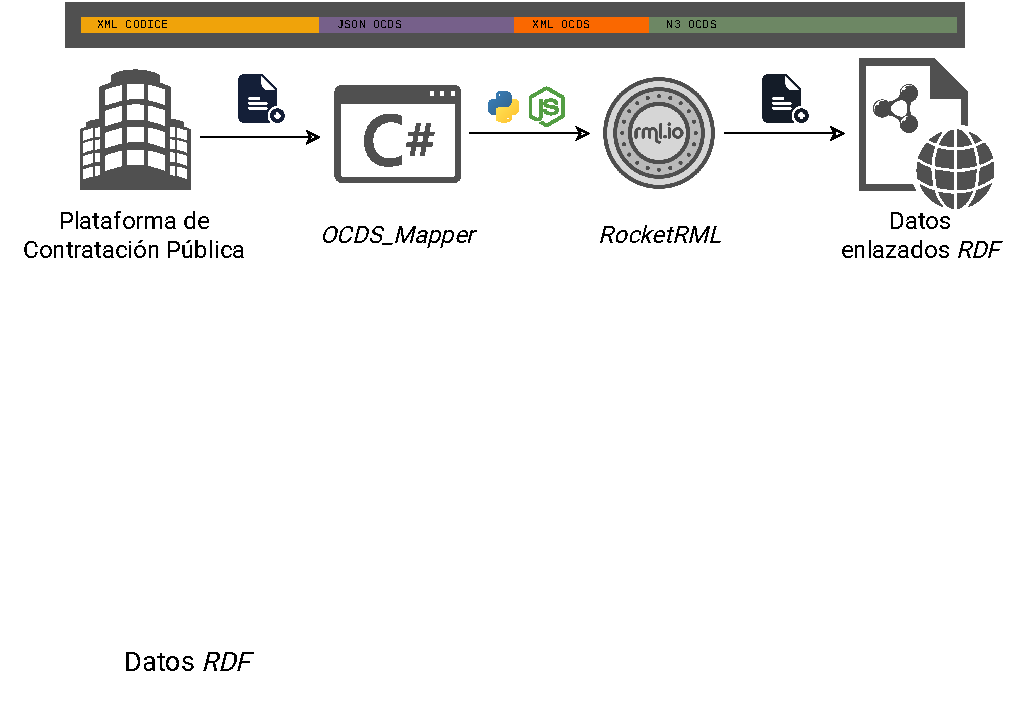
\includegraphics[width=\textwidth]{pipeline.pdf}
        \captionof{figure}{\textit{Pipeline} y formato de los datos en las distintas etapas}
        \label{fig:pipeline}
    \end{figure}
    
    \noindent En la \hyperref[fig:pipeline]{figura 21} se representa el \textit{pipeline} completo, además del formato de los datos a lo largo de las diferentes fases del procesamiento. Los datos de licitaciones originales que provienen de la Plataforma de Contratación Pública están en el formato \texttt{XML} y siguiendo el esquema \texttt{CODICE}. Una vez son procesados por el sistema \textit{OCDS\_Mapper}, éstos pasan al esquema \texttt{OCDS} y al formato \texttt{JSON}. Tras ser mapeados, se transforman mediante un sencillo script en el lenguaje \texttt{Python} (accesible en el repositorio del trabajo \cite{SCRIPTGEN}) al formato \texttt{XML} para su procesado de reglas \texttt{RML}. Éste se realiza haciendo uso de la librería \textit{RocketRML} \cite{ROCKETRML} (licencia CC-BY-SA 4.0 \cite{LICCC}), ejecutada en el entorno \texttt{Node.js}, para obtener finalmente los datos enlazados \texttt{RDF}.
    \\ \\
    Podría parecer que la transformación a \texttt{JSON} en medio del \textit{pipeline} para posteriormente volver al formato \texttt{XML} inicial es innecesaria, pero esto se hace debido a que \texttt{OCDS} requiere \texttt{JSON} como formato de sus datos, mientras que las reglas de mapeado de \texttt{RML} utilizadas están declaradas haciendo uso de \texttt{XPath}, necesitando \texttt{XML} como formato de entrada.
    
    \subsection{Validación de los datos}
        Previamente a poder realizar la transformación a datos enlazados \texttt{RDF}, es necesario validarlos para poder aseverar la correcta adecuación al estándar \texttt{OCDS} de los mismos. Para ello se ha hecho uso de la herramienta de revisión de \texttt{OCDS} \cite{OCDSREVIEWTOOL} con una batería de múltiples documentos, pero sólo se mostrará el reporte de uno cualquiera en las siguientes figuras.
        
        \begin{figure}[h]
            \centering
            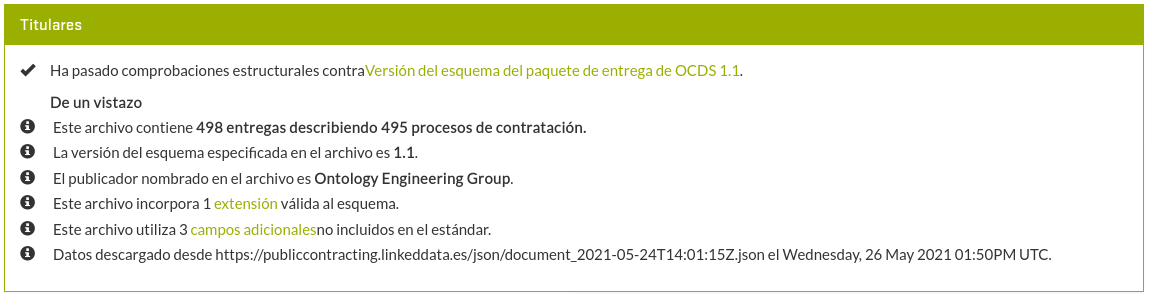
\includegraphics[width=\textwidth]{ocdsreport_1.png}
            \captionof{figure}{Reporte general de la herramienta de revisión de \texttt{OCDS}}
        \end{figure}
        
        \begin{figure}[h]
            \centering
            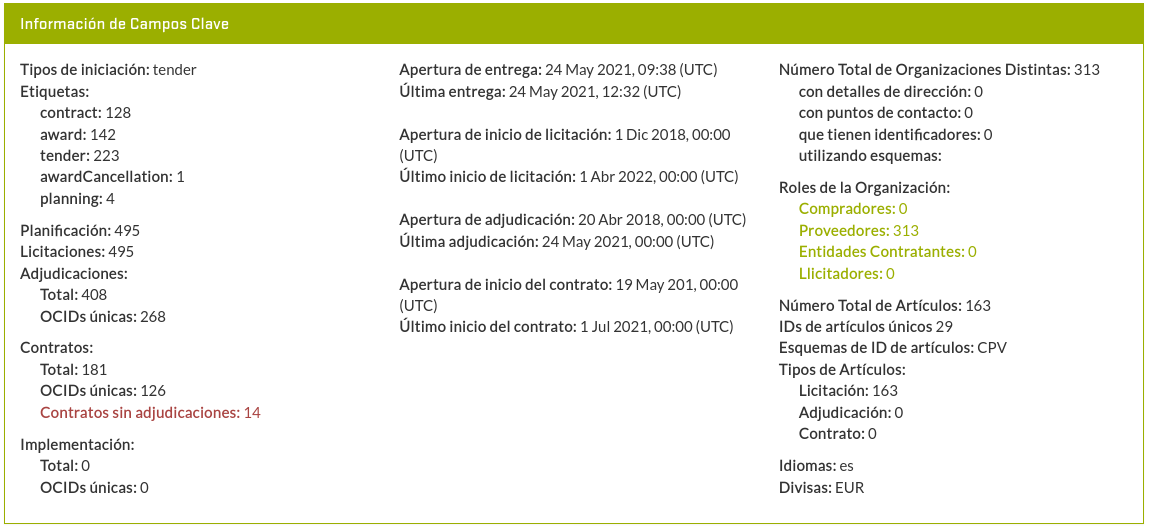
\includegraphics[width=\textwidth]{ocdsreport_2.png}
            \captionof{figure}{Reporte específico de la herramienta de revisión de \texttt{OCDS}}
        \end{figure}
        
        El reporte mostrado como ejemplo es accesible en el siguiente enlace \cite{OCDSREPORT} hasta el día 24 de agosto de 2021, gracias al acceso ofrecido durante 90 días de los reportes ejecutados por la herramienta de revisión.
        
    \subsection{Reglas \texttt{RML}}
        Para poder realizar la transformación a \textit{linked data}, se ha utilizado el lenguaje \texttt{RML} (\texttt{RDF} \textit{Mapping Language}) \cite{RML}, cuyo propósito es mapear información de muy diversas fuentes de información al sistema \texttt{RDF}.
        \\ \\
        Con respecto al procesamiento de las reglas para producir datos \texttt{RDF}, se ha valorado la utilización de dos distintos métodos de ejecución, \textit{RMLMapper} \cite{RMLMAPPER} y \textit{RocketRML} \cite{ROCKETRML}. Sin embargo, debido a la grandísima diferencia de velocidad entre ambas que se puede apreciar en la \hyperref[fig:tiemposrml]{figura 24}, favorable a \textit{RocketRML}, se ha decidido utilizar este software.
        
        \begin{figure}[!htb]
            \centering
            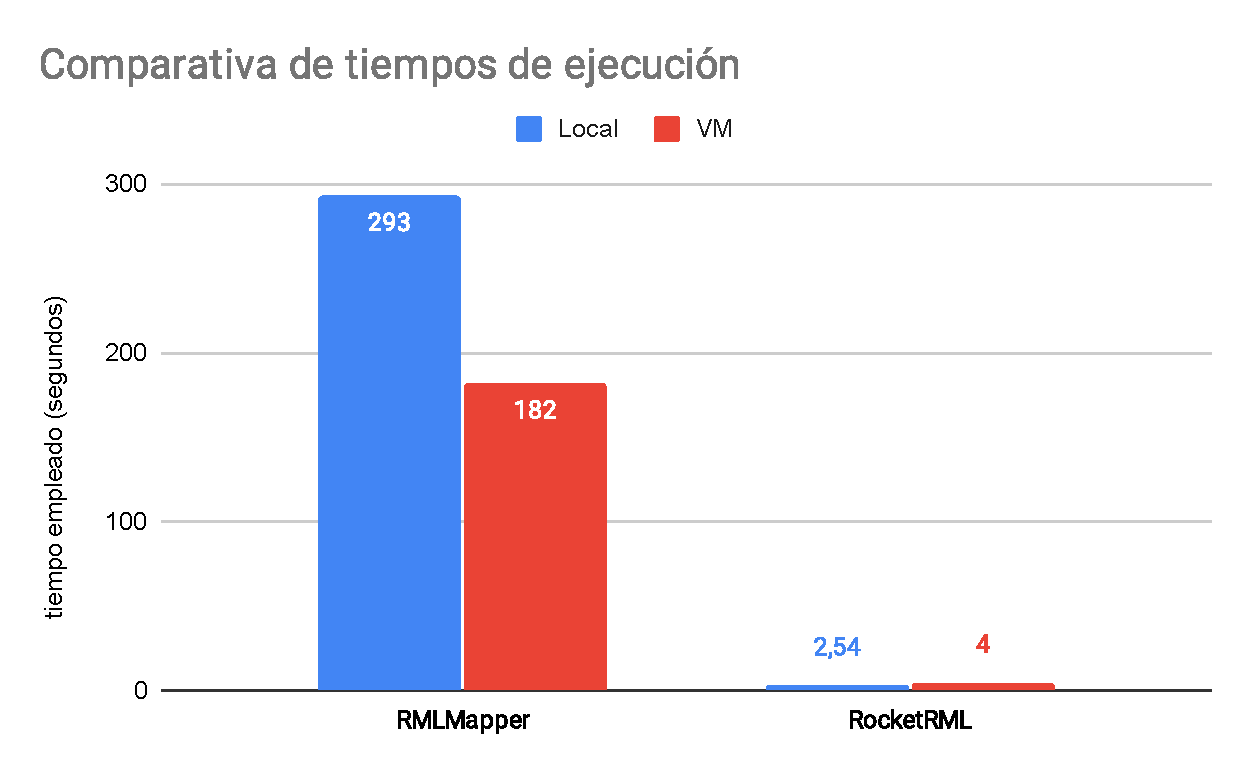
\includegraphics[width=0.7\textwidth]{tiemposrml.pdf}
            \captionof{figure}{Comparativa de tiempos entre \textit{RMLMapper} y \textit{RocketRML}}
            \label{fig:tiemposrml}
        \end{figure}
        
        \noindent Si bien es cierto que la construcción de las reglas se ha ajustado a las necesidades específicas de este proyecto, la mayor parte de éstas son una reutilización de una batería de reglas del proyecto \texttt{TBFY}, accesibles en el siguiente enlace \cite{OPENOPPSMAP}. Sobre ellas se han realizado algunas modificaciones \textit{ad-hoc}, como el cambio de las \texttt{URIs} base (de \texttt{http://data.tbfy.eu} a \texttt{https://publiccontracting.linkeddata.es}), o cambios en algunos \textit{TriplesMap}. Además, se han eliminado aquellas reglas que quedan fuera de las \hyperref[sec:correspondencias]{correspondencias} por motivos de legibilidad de las mismas y agilidad en el procesamiento. El conjunto final de reglas utilizado en el sistema desplegado es accesible en el siguiente enlace del repositorio del trabajo \cite{MYMAP}.
        
    \subsection{Consultas sobre los datos generados} \label{subsec:rdflib}
        Para comprobar que la integridad de los datos enlazados generados se ha preservado tras su procesamiento mediante las reglas \texttt{RML}, se ha confeccionado una batería de consultas \texttt{SPARQL} que asevera que toda la información codificada en dichas reglas se haya preservado.
        \\ \\
        La implementación de las consultas se ha realizado mediante un sencillo script en \texttt{Python} (accesible en el repositorio \cite{SCRIPTRDF}) haciendo uso de la librería \textit{RDFLib} (licencia BSD 3-Clause \cite{LICBSD3}). El conjunto de \textit{queries} \texttt{SPARQL} se encuentra en el \hyperref[annex:sparql]{Anexo III}.
        \\ \\
        En el repositorio del trabajo se localizan ficheros de ejemplo de la ejecución completa del \textit{pipeline} del sistema, desde los documentos originales \cite{TFGEJ1} hasta los ficheros de texto resultantes de la ejecución de las consultas descritas en esta sección \cite{TFGEJ2}, pasando por su primer procesado a \texttt{JSON} \cite{TFGEJ3} y su versión \texttt{RDF} \cite{TFGEJ4}.
        
    \subsection{Despliegue del sistema}
        Finalmente, el \textit{pipeline} completo, desde la adquisición de documentos de la Plataforma de Contratación Pública hasta la publicación de los datos enlazados ha sido desplegado en una máquina virtual provista para este propósito gracias al \textit{Ontology Engineering Group} \cite{OEG} de la UPM.
        \\ \\
        Dicha máquina virtual está compuesta por 2 procesadores Intel Xeon \texttt{CPU E5-2650 v3 @ 2.30GHz}, con 40 \textit{cores} por procesador. Cuenta asímismo con \texttt{4096 MBs} de RAM de tecnología \texttt{RDIMM} y velocidad \texttt{2133 MT/s}, y su almacenamiento es de \texttt{19 GBs}. El software de virtualización que soporta la infraestructura es \texttt{QEMU-KVM}.
        \\ \\
        En la máquina virtual, mediante el servicio Unix \texttt{cron}, se ha configurado un \textit{script} de ejecución diaria que realiza todas las etapas del procesamiento: en primer lugar, ejecuta el software \textit{OCDS\_Mapper} con el modo de operación \texttt{--daily}, dado que el servicio se ejecuta diariamente, de medianoche, y se pretenden realizar procesamientos de los datos publicados en el día anterior. Una vez se completa esa fase y se realiza el procesado a \texttt{RML} descrito en esta sección, el \textit{script} lleva al directorio \texttt{/var/www/html} dos conjuntos de ficheros: los \texttt{JSON} que devuelve el \textit{OCDS\_Mapper}, de interés por ser documentos válidos con respecto al estándar \texttt{OCDS}, y los correspondientes \texttt{N-Triples} (\texttt{RDF}) que salen de la ejecución del \textit{RocketRML}.
        \\ \\
        Una vez se han colocado los ficheros de interés en los directorios descritos, éstos quedan completamente accesibles a través de la página web \texttt{\url{https://publiccontracting.linkeddata.es}}, para su acceso y consulta.
        
        \begin{figure}[h]
            \centering
            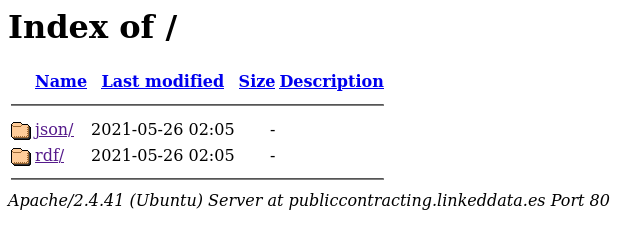
\includegraphics[width=0.755\textwidth]{index.png}
            \captionof{figure}{Captura de la web \texttt{\url{https://publiccontracting.linkeddata.es}}}
        \end{figure}
        
        \begin{figure}[!htb]
            \centering
            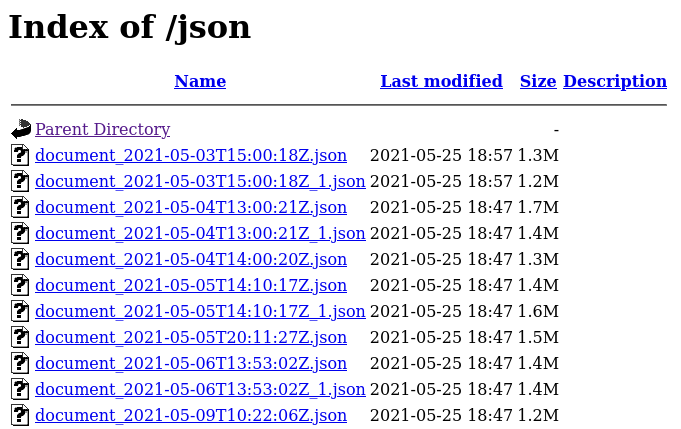
\includegraphics[width=0.755\textwidth]{index_json.png}
            \captionof{figure}{Captura de parte del directorio \texttt{json/} de la web}
        \end{figure}
        
    \vspace{2cm}
    
        \begin{figure}[!htb]
            \centering
            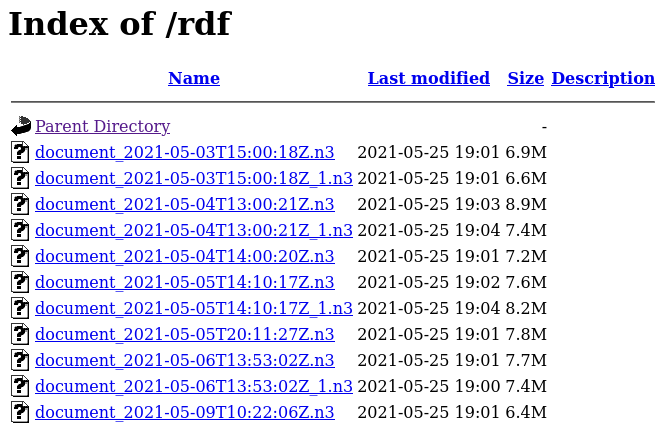
\includegraphics[width=0.755\textwidth]{index_rdf.png}
            \captionof{figure}{Captura de parte del directorio \texttt{rdf/} de la web}
        \end{figure}
    
\newpage
    \mysection{Análisis del impacto del trabajo}

    Según lo previamente descrito y los resultados provistos por este trabajo, se pretende que éste tenga una fuerte componente práctica en el ámbito de la información de las licitaciones públicas. Por ello, se espera que el impacto de este trabajo sea significativo en este campo, el de los datos abiertos, que además tiene como algunas de sus bases fundamentales la cooperación e interoperabilidad de sistemas con el fin de proveer servicios que puedan ser accedidos y aprovechados por todos.
    \\ \\
    Si bien es cierto que el funcionamiento del sistema desarrollado y desplegado en este trabajo se basa fundamentalmente en la transformación de datos, se espera que gracias a esta transformación y a su publicación como datos enlazados se pueda construir y mejorar la base de conocimiento existente acerca del ámbito de las licitaciones de tal manera que sirva tanto de apoyo en la toma de decisiones de las entidades públicas, como de disuasión de algunos delitos fiscales que puedan ser encontrados mediante la explotación de los nuevos datos.
    \\ \\
    En relación con los Objetivos de Desarrollo Sostenible de la Agenda 2030 de la Organización de las Naciones Unidas \cite{ODS}, este trabajo se alinea con el objetivo decimosexto, \texttt{ODS 16} - \textit{Promover sociedades pacíficas e inclusivas para el desarrollo sostenible, facilitar el acceso a la justicia para todos y crear instituciones eficaces, responsables e inclusivas a todos los niveles} \cite{ODS16}. Según lo expuesto en los dos anteriores párrafos, se espera que este trabajo sirva para mejorar la eficacia de las instituciones públicas, en este caso de aquellas relacionadas con las ofertas de contrataciones.
    \\ \\
    
    \begin{figure}[h]
        \centering
        
\includegraphics[width=0.625\textwidth]{ods16.jpeg}
        \captionof{figure}{Logo del Objetivo de Desarrollo Sostenible nº 16}
    \end{figure}

\newpage
    \mysection{Conclusiones}

    ...

\newpage
    \section{Referencias}

\begingroup
    \renewcommand{\section}[2]{}%
    \begin{thebibliography}{X}
    
        \bibitem{OPENDATA}
            Open Knowledge Foundation,
            \\ \textit{Open Data Handbook: ¿Qué son los datos abiertos?}.
            \\ \texttt{\url{https://opendatahandbook.org/guide/es/what-is-open-data/}}
            
        \bibitem{LINKEDDATA}
            World Wide Web Consortium,
            \\ \textit{Guía breve de Linked Data}.
            \\ \texttt{\url{https://www.w3c.es/Divulgacion/GuiasBreves/LinkedData}}
            
        \bibitem{LOD}
            The Linked Open Data Cloud.
            \\ \texttt{\url{https://lod-cloud.net/}}
            
        \bibitem{HTML}
            Web Hypertext Application Technology Working Group,
            \\ \textit{HTML Living Standard}.
            \\ \texttt{\url{https://html.spec.whatwg.org/multipage/}}
            
        \bibitem{RDF}
            World Wide Web Consortium,
            \\ \textit{RDF 1.1 Concepts and Abstract Syntax}.
            \\ \texttt{\url{https://www.w3.org/TR/rdf11-concepts/}}
        
        \bibitem{DBPEDIA}
            DBpedia.
            \\ \texttt{\url{https://www.dbpedia.org/}}
        
        \bibitem{LOV}
            Linked Open Vocabularies.
            \\ \texttt{\url{https://lov.linkeddata.es/dataset/lov}}
        
        \bibitem{NTRIPLES}
            World Wide Web Consortium,
            \\ \textit{RDF 1.1 N-Triples, A line-based syntax for an RDF graph}.
            \\ \texttt{\url{http://www.w3.org/TR/n-triples/}}
        
        \bibitem{TURTLE}
            World Wide Web Consortium,
            \\ \textit{RDF 1.1 Turtle, Terse RDF Triple Language}.
            \\ \texttt{\url{https://www.w3.org/TR/turtle/}}
            
        \bibitem{JSONLD}
            World Wide Web Consortium,
            \\ \textit{JSON-LD 1.1, A JSON-based Serialization for Linked Data}.
            \\ \texttt{\url{http://www.w3.org/TR/json-ld/}}
        
        \bibitem{RDFXML}
            World Wide Web Consortium,
            \\ \textit{RDF 1.1 XML Syntax}.
            \\ \texttt{\url{https://www.w3.org/TR/rdf-syntax-grammar/}}
            
        \bibitem{RDFA}
            World Wide Web Consortium,
            \\ \textit{RDFa 1.1 Primer - Third Edition, Rich Structured Data Markup for Web Documents}.
            \\ \texttt{\url{https://www.w3.org/TR/xhtml-rdfa-primer/}}
            
        \bibitem{NQUADS}
            World Wide Web Consortium,
            \\ \textit{RDF 1.1 N-Quads, A line-based syntax for RDF datasets}.
            \\ \texttt{\url{https://www.w3.org/TR/n-quads/}}
            
        \bibitem{ISOSQL}
            International Organization for Standardization,
            \\ \textit{Information processing systems — Database language — SQL}.\\
            ISO 9075:1987
            \\ \texttt{\url{https://www.iso.org/standard/16661.html}}
            
        \bibitem{SPARQL}
            World Wide Web Consortium,
            \\ \textit{SPARQL Query Language for RDF}.
            \\ \texttt{\url{https://www.w3.org/TR/rdf-sparql-query/}}
            
        \bibitem{JENA}
            The Apache Software Foundation,
            \\ \textit{A free and open source Java framework for building Semantic Web and Linked Data applications}.
            \\ \texttt{\url{https://jena.apache.org/}}
            
        \bibitem{RDFLIB}
            RDFLib Team,
            \\ \textit{Python library for working with RDF, a simple yet powerful language for representing information}.
            \\ \texttt{\url{https://github.com/RDFLib/rdflib}}
            
        \bibitem{RDF4J}
            Eclipse Foundation, Inc.,
            \\ \textit{Scalable RDF for Java}.
            \\ \texttt{\url{https://rdf4j.org/}}
            
        \bibitem{VIRTUOSO}
            OpenLink Software,
            \\ \textit{SQL-ORDBMS and Web Server hybrid with RDF data management}.
            \\ \texttt{\url{https://virtuoso.openlinksw.com/}}
            
        \bibitem{UE201423}
            Diario Oficial de la Unión Europea,
            \\ \textit{Directiva 2014/23/UE del Parlamento Europeo y del Consejo de 26 de febrero de 2014 relativa a la adjudicación de contratos de concesión}.
            \\ \texttt{\url{https://eur-lex.europa.eu/legal-content/ES/TXT/PDF/?uri=CELEX:32014L0023&from=ES}}
            
        \bibitem{UE201424}
            Diario Oficial de la Unión Europea,
            \\ \textit{Directiva 2014/24/UE del Parlamento Europeo y del Consejo de 26 de febrero de 2014 sobre contratación pública}.
            \\ \texttt{\url{https://eur-lex.europa.eu/legal-content/ES/TXT/PDF/?uri=CELEX:32014L0024&from=ES}}
            
        \bibitem{UE201425}
            Diario Oficial de la Unión Europea,
            \\ \textit{Directiva 2014/25/UE del Parlamento Europeo y del Consejo de 26 de febrero de 2014 relativa a la contratación por entidades que operan en los sectores del agua, la energía, los transportes y los servicios postales}.
            \\ \texttt{\url{https://eur-lex.europa.eu/legal-content/ES/TXT/PDF/?uri=CELEX:32014L0025&from=ES}}
            
        \bibitem{UE200981}
            Diario Oficial de la Unión Europea,
            \\ \textit{Directiva 2009/81/CE del Parlamento Europeo y del Consejo de 13 de julio de 2009 sobre coordinación de los procedimientos de adjudicación de determinados cnotratos de obras, de sumistro y de servicios por las entidades o poderes adjudicadores en los ámbitos de la defensa y la seguridad}.
            \\ \texttt{\url{https://eur-lex.europa.eu/legal-content/ES/TXT/PDF/?uri=CELEX:32009L0081&from=ES}}
            
        \bibitem{BOE20179}
            Boletín Oficial del Estado,
            \\ \textit{Ley 9/2017, de 8 de noviembre, de Contratos del Sector Público, por la que se transponen al ordenamiento jurídico español las Directivas del Parlamento Europeo y del Consejo 2014/23/UE y 2014/24/UE, de 26 de febrero de 2014}.
            \\ \texttt{\url{https://www.boe.es/buscar/pdf/2017/BOE-A-2017-12902-consolidado.pdf}}
            
        \bibitem{CODICEIMPL}
            Ministerio de Hacienda,
            \\ \textit{Guía de implementación de documentos CODICE 2.0}.
            \\ \texttt{\url{https://contrataciondelestado.es/codice/2.0/doc/CODICE_2_GuiaImplementacion_v1.3.pdf}}
            
        \bibitem{CODICEFORM}
            Ministerio de Hacienda,
            \\ \textit{Formato de sindicación y reutilización de datos sobre licitaciones publicadas en la Plataforma de Contratación del Sector Público}.
            \\ \texttt{\url{https://www.hacienda.gob.es/Documentacion/Publico/D.G. PATRIMONIO/Plataforma_Contratacion/especificacion-sindicacion-1-3.pdf}}
            
        \bibitem{ISOMDR}
            International Organization for Standardization,
            \\ \textit{Information technology — Metadata registries (MDR) — Part 7: Metamodel for data set registration}.\\
            ISO/IEC 11179-7:2019
            \\ \texttt{\url{https://www.iso.org/standard/68766.html}}
            
        \bibitem{ISOEBXML}
            International Organization for Standardization,
            \\ \textit{Electronic Business Extensible Markup Language (ebXML) — Part 5: Core Components Specification (CCS)}.\\
            ISO 15000-5:2014
            \\ \texttt{\url{https://www.iso.org/standard/61433.html}}
            
        \bibitem{EBXML}
            OASIS,
            \\ \textit{Electronic Business using eXtensible Markup Language}.
            \\ \texttt{\url{http://www.ebxml.org/l}}
            
        \bibitem{UNCEFACT}
            Comisión Económica de las Naciones Unidas para Europa,
            \\ \textit{Trade Facilitation and E-business}.
            \\ \texttt{\url{https://unece.org/trade/uncefact}}
            
        \bibitem{XML}
            World Wide Web Consortium,
            \\ \textit{Extensible Markup Language (XML)}.
            \\ \texttt{\url{https://www.w3.org/XML/}}
            
        \bibitem{UEIDA}
            Diario Oficial de las Comunidades Europeas,
            \\ \textit{Intercambio electrónico de datos entre administraciones: Programa IDA}.
            \\ \texttt{\url{https://eur-lex.europa.eu/legal-content/ES/TXT/HTML/?uri=LEGISSUM:l24147a&from=ES}}
            
        \bibitem{CODICE}
            Portal de Administración Electrónica,
            Ministerio de Asuntos Económicos y Transformación Digital,
            \\ \textit{Componentes y Documentos Interoperables para la Contratación Electrónica}.
            \\ \texttt{\url{https://administracionelectronica.gob.es/cise/137}}
            
        \bibitem{PORTALHAC}
            Ministerio de Hacienda,
            \\ \textit{Licitaciones publicadas en la Plataforma de Contratación del Sector Público}.
            \\ \texttt{\url{https://www.hacienda.gob.es/es-ES/GobiernoAbierto/Datos Abiertos/Paginas/licitaciones\_plataforma\_contratacion.aspx}}
            
        \bibitem{CODICETIPOS}
            Ministerio de Hacienda,
            \\ \textit{Resumen de contenido en conjuntos de datos abiertos}.
            \\ \texttt{\url{https://www.hacienda.gob.es/Documentacion/Publico/D.G. PATRIMONIO/Plataforma_Contratacion/Resumen-Datos-Abiertos.pdf}}
            
        \bibitem{OCDS}
            Open Contracting Partnership,
            \\ \textit{Estándar de Datos de Contrataciones Abiertas: Documentación}.
            \\ \texttt{\url{https://standard.open-contracting.org/latest/es/\#}}
        
        \bibitem{OCDSTOOLS}
            Open Contracting Partnership,
            \\ \textit{Open Contracting Tools Directory}.
            \\ \texttt{\url{https://www.open-contracting.org/es/resources/open-contracting-tools-directory/}}
            
        \bibitem{OCDSOC}
            Open Contracting Partnership,
            \\ \textit{El Estándar de Datos para las Contrataciones Abiertas}.
            \\ \texttt{\url{https://www.open-contracting.org/es/data-standard/}}
            
        \bibitem{OCDSBLOCKS}
            Open Contracting Partnership,
            \\ \textit{Estándar de Datos de Contrataciones Abiertas: Bloques}.
            \\ \texttt{\url{https://standard.open-contracting.org/latest/es/getting_started/building_blocks/}}
    
        \bibitem{JSTD}
            Institute of Electrical and Electronics Engineers,
            \\ \textit{Standard for Information Technology Software Life Cycle Processes Software Development Acquirer-Supplier Agreement}.
            \\ \texttt{\url{https://ieeexplore.ieee.org/document/6569022}}
    
        \bibitem{ISOCS}
            International Organization for Standardization,
            \\ \textit{Information technology — Programming languages — C\#}.\\
            ISO/IEC 23270:2018
            \\ \texttt{\url{https://www.iso.org/standard/75178.html}}
        
        \bibitem{LINQXML}
            Microsoft,
            \\ \textit{LINQ to XML overview}.
            \\ \texttt{\url{https://docs.microsoft.com/en-us/dotnet/standard/linq/linq-xml-overview}}
        
        \bibitem{LIBASYNC}
            Stephen Cleary,
            \\ \textit{A helper library for async/await}.
            \\ \texttt{\url{https://github.com/StephenCleary/AsyncEx}}
        
        \bibitem{LIBASSERT}
            Dennis Doomen,
            \\ \textit{Fluent API for asserting the results of unit tests that targets .NET Framework}.
            \\ \texttt{\url{https://fluentassertions.com/}}
        
        \bibitem{LIBLOG4}
            The Apache Software Foundation,
            \\ \textit{A port of the original Apache log4j framework to the Microsoft .NET Framework}.
            \\ \texttt{\url{https://logging.apache.org/log4net/}}
        
        \bibitem{LIBCONFIG}
            Microsoft,
            \\ \textit{Implementation of key-value pair based configuration}.
            \\ \texttt{\url{https://github.com/dotnet/runtime/tree/main/src/libraries/Microsoft.Extensions.Configuration}}
        
        \bibitem{LIBJSON}
            Newtonsoft,
            \\ \textit{Popular high-performance JSON framework for .NET Framework}.
            \\ \texttt{\url{https://www.newtonsoft.com/json}}
        
        \bibitem{LIBXUNIT}
            .NET Foundation,
            \\ \textit{Free, open source, community-focused unit testing tool for the .NET Framework}.
            \\ \texttt{\url{https://xunit.net/}}
        
        \bibitem{VSPROJSOL}
            Microsoft,
            \\ \textit{Introducción a proyectos y soluciones}.
            \\ \texttt{\url{https://docs.microsoft.com/es-es/visualstudio/get-started/tutorial-projects-solutions?view=vs-2019}}
        
        \bibitem{LICIDIA}
            Ministerio de Hacienda,
            \\ \textit{Documento de licitaciones de actualización diaria}.
            \\ \texttt{\url{https://contrataciondelestado.es/sindicacion/sindicacion\_643/licitacionesPerfilesContratanteCompleto3.atom}}
            
        \bibitem{SONARQUBE}
            SonarSource,
            \\ \textit{SonarQube}.
            \\ \texttt{\url{https://www.sonarqube.org/}}
        
        \bibitem{CHECKLIST}
            Yo?,
            \\ \textit{CODICE-OCDS Mappings}.
            \\ \texttt{\url{https://docs.google.com/spreadsheets/d/14pikYzS-yzNWjtISyU-bPtoPe7cY1-KjOGGSC0lBhnI/edit?usp=sharing}}
        
        \bibitem{CR1}
            Ministerio de Hacienda,
            \\ \textit{Codigos de estados de licitación definidos por la DGPE para la sindicacion entre plataformas}.
            \\ \texttt{\url{https://contrataciondelestado.es/codice/cl/2.04/SyndicationContractFolderStatusCode-2.04.gc}}
            
        \bibitem{CR2}
            Open Contracting Partnership,
            \\ \textit{Listas de códigos - Etiqueta de entrada}.
            \\ \texttt{\url{https://standard.open-contracting.org/latest/es/schema/codelists/\#release-tag}}
            
        \bibitem{CR3}
            Ministerio de Hacienda,
            \\ \textit{Codigos de tipos de contrato definidos por la DGPE para la sindicacion entre plataformas}.
            \\ \texttt{\url{https://contrataciondelestado.es/codice/cl/2.08/ContractCode-2.08.gc}}
            
        \bibitem{CR4}
            Open Contracting Partnership,
            \\ \textit{Listas de códigos - Categoría de compra}.
            \\ \texttt{\url{https://standard.open-contracting.org/latest/es/schema/codelists/\#procurement-category}}
            
        \bibitem{CR5}
            Open Contracting Partnership,
            \\ \textit{Listas de códigos - Tipo de documento}.
            \\ \texttt{\url{https://standard.open-contracting.org/latest/es/schema/codelists/\#document-type}}
            
        \bibitem{CR6}
            Open Contracting Partnership,
            \\ \textit{OCDS Extension Explorer - Lots}.
            \\ \texttt{\url{https://extensions.open-contracting.org/en/extensions/lots/v1.1.5/}}
            
        \bibitem{CR7}
            PublicTendering,
            \\ \textit{List of the CPV codes}.
            \\ \texttt{\url{https://www.publictendering.com/cpv-codes/list-of-the-cpv-codes/}}
            
        \bibitem{CR8}
            Ministerio de Hacienda,
            \\ \textit{Codigos de tipos de procedimientos de contratación definidos por la DGPE para la sindicacion entre plataformas}.
            \\ \texttt{\url{https://contrataciondelestado.es/codice/cl/2.07/SyndicationTenderingProcessCode-2.07.gc}}
            
        \bibitem{CR9}
            Open Contracting Partnership,
            \\ \textit{Listas de códigos - Método}.
            \\ \texttt{\url{https://standard.open-contracting.org/latest/es/schema/codelists/\#method}}
            
        \bibitem{CR10}
            Ministerio de Hacienda,
            \\ \textit{Codigos de tipos de sistemas de contratación definidos por la DGPE para la sindicacion entre plataformas}.
            \\ \texttt{\url{https://contrataciondelestado.es/codice/cl/2.08/ContractingSystemTypeCode-2.08.gc}}
            
        \bibitem{CR11}
            Ministerio de Hacienda,
            \\ \textit{Codigos de tipos de presentación de oferta definidos por la DGPE para la sindicacion entre plataformas}.
            \\ \texttt{\url{https://contrataciondelestado.es/codice/cl/1.04/TenderDeliveryCode-1.04.gc}{enlace}}
            
        \bibitem{CR12}
            Open Contracting Partnership,
            \\ \textit{Listas de códigos - Método de presentación}.
            \\ \texttt{\url{https://standard.open-contracting.org/latest/es/schema/codelists/\#submission-method}}
            
        \bibitem{CR13}
            Open Contracting Partnership,
            \\ \textit{Listas de códigos - Esquema de Identificación de Organizaciones}.
            \\ \texttt{\url{https://standard.open-contracting.org/latest/es/schema/codelists/\#organization-identifier-scheme}}
            
        \bibitem{CR14}
            Open Data Services,
            \\ \textit{Common Directory of Organizational Units and Offices - DIR3}.
            \\ \texttt{\url{http://org-id.guide/list/ES-DIR3}}
            
        \bibitem{CR15}
            Open Data Services,
            \\ \textit{Central Commercial Register of the Kingdom of Spain - RMC}.
            \\ \texttt{\url{http://org-id.guide/list/ES-RMC}}
        
        \bibitem{CR16}
            Ministerio de Hacienda,
            \\ \textit{Codigos de resultados de licitaciones definidos por la DGPE para la sindicacion entre plataformas}.
            \\ \texttt{\url{http://contrataciondelestado.es/codice/cl/2.02/TenderResultCode-2.02.gc}}
            
        \bibitem{CR17}
            Open Contracting Partnership,
            \\ \textit{Listas de códigos - Estado de la adjudicación}.
            \\ \texttt{\url{https://standard.open-contracting.org/latest/es/schema/codelists/\#award-status}}
            
        \bibitem{CR18}
            Open Contracting Partnership,
            \\ \textit{Listas de códigos - Rol de la parte}.
            \\ \texttt{\url{https://standard.open-contracting.org/latest/es/schema/codelists/\#party-role}}
        
    \end{thebibliography}
\endgroup

\newpage
    \mysection{Anexos}

    \subsection{Anexo I: Interfaces de los componentes del \textit{OCDS\_Mapper}}
        \subsubsection{Componente \textit{Provider}}
            \begin{lstlisting}[language=lCSharp]
                namespace OCDS_Mapper.src.Interfaces
                {
                    /* Interfaz del componente de provisión de datos */
                
                    public interface IProvider
                    {
                        /* Propiedades */
                
                        /*  propiedad Parser => IParser
                         *      Instancia del Parser para obtener los enlaces de los documentos
                         */
                        IParser Parser { get; set; }
                
                        /*  propiedad Files => AsyncCollection<Document>
                         *      Colección thread-safe que permite una extracción
                         *      ordenada de los documentos provistos
                         */
                        AsyncCollection<Document> Files { get; set; }
                
                
                        /* Funciones */
                
                        /*  función asíncrona TakeFile() => Document
                         *      Función bloqueante que devuelve un documento provisto cuando éste
                         *      está disponible
                         *  @return : stream de texto del documento provisto, o null si no quedan
                         *      más documentos que proveer
                         */
                        Task<Document> TakeFile();
                
                        /*  función SetParser(IParser) => bool
                         *      (utilizada solo en modo PROVIDE_ALL y PROVIDE_DAILY)
                         *      Desbloquea el thread en background que integra al Provider y al Parser
                         *  @param parser : Instancia del Parser para cada documento
                         *  @return : true si el documento del Parser es día anterior al actual,
                         *      false e.o.c
                         */
                        bool SetParser(IParser parser);
                
                        /*  función RemoveFile(string) => void
                         *      Función que elimina un archivo provisto ya mapeado
                         *  @param filePath : path del documento a eliminar
                         */
                        void RemoveFile(string filePath);
                    }
                }
            \end{lstlisting}
\newpage
        \subsubsection{Componente \textit{Parser}}
            \begin{lstlisting}[language=lCSharp]
                namespace OCDS_Mapper.src.Interfaces
                {
                    /* Interfaz del componente de parseo */
                    
                    public interface IParser
                    {
                        /* Propiedades */
                
                        /*  propiedad DocumentRoot => XElement
                         *      Representa el elemento XML raíz del documento atom
                         */
                        XElement DocumentRoot { get; set; }
                
                        /*  propiedad EntryRoot => XElement
                         *      Representa el elemento XML raíz de la entrada siendo parseada:
                         *      @ej : XElement(<cac-place-ext:ContractFolderStatus>)
                         */
                        XElement EntryRoot { get; set; }
                
                
                        /* Funciones */
                
                        /*  función GetNamespaces() => IDictionary<string, XNamespace>
                         *      Representa mediante pares de nombres y espacios de nombres los 
                         *      namespaces del documento
                         *      Recupera dicha información de los atributos del elemento feed en los
                         *      ficheros atom
                         *  @return : Diccionario con los pares de espacios de nombres
                         *      @ej : { {"cac" : XNamespace("...:CommonAggregateComponents-2")}, ... }
                         */
                        IDictionary<string, XNamespace> GetNamespaces();
                
                        /*  función GetEntrySet(IDictionary<string, XNamespace>) => IEnumerable<XElement>
                         *      Devuelve el conjunto de entradas en el fichero atom
                         *      Las entradas vienen definidas por el elemento entry
                         *  @param namespaces : Diccionario de espacios de nombres
                         *  @return : Conjunto de elementos XML
                         *      @ej : [ XElement(<entry xmlns="..."> <id>...</id> ... </entry>), ... ]
                         */
                        IEnumerable<XElement> GetEntrySet(IDictionary<string, XNamespace> namespaces);
                
                        /*  función SetEntryRootElement(XElement) => void
                         *      Actualiza la propiedad del objeto EntryRoot
                         *      Extrae el elemento XML correspondiente a "ContractFolderStatus"
                         *  @throws InvalidParsedElementException : si el elemento no contiene 
                         *      "ContractFolderStatus"
                         */
                        void SetEntryRootElement(XElement entry);
                
                
                
                
                        /*  función GetElements(IEnumerable<XName>) => XElement[]
                         *      Devuelve el (los) elemento(s) XML descrito por la ruta pasada
                         *      como parámetro
                         *  @param pathToElement : lista enlazada con la ruta del elemento deseado:
                         *      @ej : [ XName(XNamespace("cac") + "ProcurementProject"),
                         *              XName(XNamespace("cbc") + "Name") ]
                         *  @return : elemento(s) buscado(s), o null si no se puede encontrar
                         *      @ej : XElement(<cbc:Name>"..."</cbc:Name>)
                         */
                        XElement[] GetElements(IEnumerable<XName> pathToElement);
                
                        /*  función GetNextFile() => Uri
                         *      Devuelve la URI correspondiente al siguiente fichero, descrito por el
                         *      elemento "link" y el atributo "rel=next"
                         *  @return : La URI que describe el fichero enlazado al siendo parseado en
                         *      esta instancia
                         */
                        Uri GetNextFile();
                
                        /*  función GetDocumentTimestamp(bool) => string
                         *      Devuelve el timestamp del documento o de una entrada específica
                         *  @param document : True si se quiere recuperar el timestamp del documento, 
                         *      False si se quiere el de la entrada
                         *  @return : timestamp (o campo "updated") del documento de licitaciones
                         *      o de la entrada
                         */
                        string GetDocumentTimestamp(bool document);
                    }
                }
            \end{lstlisting}
\newpage
        \subsubsection{Componente \textit{Mapper}}
            \begin{lstlisting}[language=lCSharp]
                namespace OCDS_Mapper.src.Interfaces
                {
                    /* Interfaz del componente de mapeo */
                
                    public interface IMapper
                    {
                        /* Propiedades */
                
                        /*  propiedad MappedEntry => JObject
                         *      Representa el elemento JSON con la información mapeada
                         */
                        JObject MappedEntry { get; set; }
                
                
                        /* Funciones */
                
                        /*  función MapElement(IEnumerable<string>, XElement[]) => void
                         *      Realiza el mapeo de elemento(s) CODICE a elemento(s) OCDS
                         *  @param pathMap : ruta del elemento cuando sea mapeado
                         *  @param parsedElement : elemento(s) a mapear
                         *  @ej : MapElement( [ "tender", "title" ], [ "ABCD" ] )
                         *      => MappedEntry = { "tender": { "title": "ABCD" } }
                         *  @ej : MapElement( [ "tag" ], [ "PRE" ] )
                         *      => MappedEntry = { "tag": [ "planning" ] }
                         */
                        void MapElement(IEnumerable<string> pathMap, XElement[] parsedElement);
                
                        /*  función Commit(string) => void
                         *      Introduce los cambios al JSON que no se pueden introducir
                         *      mediante los mapeos unitarios de elementos (metadatos, colecciones, etc.)
                         *  @param publishDate : fecha de publicación de la entrega
                         */
                        void Commit(string publishDate);
                    }
                }
            \end{lstlisting}
\newpage
        \subsubsection{Componente \textit{Packager}}
            \begin{lstlisting}[language=lCSharp]
                namespace OCDS_Mapper.src.Interfaces
                {
                    /* Interfaz del componente de empaquetado de datos  */
                
                    public interface IPackager
                    {
                        /* Funciones */
                
                        /*  función GetIdentifier(string) => string
                         *      Obtiene el número de ocurrencias del identificador hasta el momento
                         *      con el objetivo de evitar colisiones de ids no únicos
                         *  @param entryID : identificador de la entrada
                         *  @return : número de ocurrencias del identificador
                         */
                        string GetIdentifier(string entryID);
                
                        /*  función Package(JObject) => void
                         *      Introduce una entrada al paquete
                         *  @param entry : objeto JSON que introducir
                         */
                        void Package(JObject entry);
                
                        /*  función Publish(string) => void
                         *      Publica los datos escribiéndolos en el directorio de salida
                         *  @param dirPath : path del directorio de salida
                         */
                        void Publish(string dirPath);
                    }
                }
            \end{lstlisting}
            
\newpage

    \subsection{Anexo II: Ejemplos de los mapeados entre \texttt{CODICE} y \texttt{OCDS}}

        \subsubsection{Datos generales del expediente}
            \paragraph{Estado} \mbox{}\\
                \begin{lstlisting}[language=lXML]
                    <cac-place-ext:ContractFolderStatus>
                        <cbc-place-ext:ContractFolderStatusCode languageID="es"
                         listURI="https://contrataciondelestado.es/codice/cl/2.04/
                         SyndicationContractFolderStatusCode-2.04.gc">
                            ADJ
                        </cbc-place-ext:ContractFolderStatusCode>
                    </cac-place-ext:ContractFolderStatus>
                \end{lstlisting}
                
                \begin{center}
                    $\big\Downarrow$
                \end{center}
                
                \begin{lstlisting}[language=lJSON]
                    {
                        "tag": [
                            "award"
                        ]
                    }
                \end{lstlisting}
                
            \paragraph{Número de expediente} \mbox{}\\
                \begin{lstlisting}[language=lXML]
                    <cac-place-ext:ContractFolderStatus>
                        <cbc:ContractFolderID>
                            002/2021-CONTR
                        </cbc:ContractFolderID>
                    </cac-place-ext:ContractFolderStatus>
                \end{lstlisting}
                
                \begin{center}
                    $\big\Downarrow$
                \end{center}
                
                \begin{lstlisting}[language=lJSON]
                    {
                        "ocid": "ES-002/2021-CONTR"
                    }
                \end{lstlisting}
                
            \paragraph{Objeto del contrato} \mbox{}\\
                \begin{lstlisting}[language=lXML]
                    <cac-place-ext:ContractFolderStatus>
                        <cac:ProcurementProject>
                            <cbc:Name>
                                Suministro de energía eléctrica para las instalaciones de RTVE
                            </cbc:Name>
                        </cac:ProcurementProject>
                    </cac-place-ext:ContractFolderStatus>
                \end{lstlisting}
                
                \begin{center}
                    $\big\Downarrow$
                \end{center}
                
                \begin{lstlisting}[language=lJSON]
                    {
                        "tender": {
                            "title": "Suministro de energía eléctrica para las instalaciones de RTVE"
                        }
                    }
                \end{lstlisting}
                
            \paragraph{Valor estimado e importe de licitación} \mbox{}\\
                \begin{lstlisting}[language=lXML]
                    <cac-place-ext:ContractFolderStatus>
                        <cac:ProcurementProject>
                            <cac:BudgetAmount>
                                <cbc:EstimatedOverallContractAmount currencyID="EUR">
                                    185000
                                </cbc:EstimatedOverallContractAmount>
                                <cbc:TotalAmount currencyID="EUR">
                                    120000
                                </cbc:TotalAmount>
                            </cac:BudgetAmount>
                        </cac:ProcurementProject>
                    </cac-place-ext:ContractFolderStatus>
                \end{lstlisting}
                
                \begin{center}
                    $\big\Downarrow$
                \end{center}
                
                \begin{lstlisting}[language=lJSON]
                    {
                        "tender": {
                            "value": {
                                "amount": 185000,
                                "currency": "EUR"
                            }
                        } ,
                        "planning": {
                            "budget": {
                                "amount": {
                                    "amount": 120000,
                                    "currency": "EUR"
                                }
                            }
                        }
                    }
                \end{lstlisting}
\newpage
            \paragraph{Duración del contrato} \mbox{}\\
                \begin{lstlisting}[language=lXML]
                    <cac-place-ext:ContractFolderStatus>
                        <cac:ProcurementProject>
                            <cac:PlannedPeriod>
                                <cbc:StartDate>
                                    2021-09-01
                                </cbc:StartDate>
                                <cbc:EndDate>
                                    2021-12-01
                                </cbc:EndDate>
                            </cac:PlannedPeriod>
                        </cac:ProcurementProject>
                    </cac-place-ext:ContractFolderStatus>
                \end{lstlisting}
                
                \begin{center}
                    $\big\Downarrow$
                \end{center}
                
                \begin{lstlisting}[language=lJSON]
                    {
                        "tender": {
                            "tenderPeriod": {
                                "startDate": "2021-09-01T00:00:00Z",
                                "endDate": "2021-12-01T00:00:00Z"
                            }
                        }
                    }
                \end{lstlisting}
                
                \begin{lstlisting}[language=lXML]
                    <cac-place-ext:ContractFolderStatus>
                        <cac:ProcurementProject>
                            <cac:PlannedPeriod>
                                <cbc:DurationMeasure unitCode="MON">
                                    3
                                </cbc:DurationMeasure>
                            </cac:PlannedPeriod>
                        </cac:ProcurementProject>
                    </cac-place-ext:ContractFolderStatus>
                \end{lstlisting}
                
                
                \begin{center}
                    $\big\Downarrow$
                \end{center}
                
                \begin{lstlisting}[language=lJSON]
                    {
                        "tender": {
                            "tenderPeriod": {
                                "durationInDays": 90
                            }
                        }
                    }
                \end{lstlisting}
            
            \paragraph{Tipo de contrato} \mbox{}\\
                \begin{lstlisting}[language=lXML]
                    <cac-place-ext:ContractFolderStatus>
                        <cac:ProcurementProject>
                            <cbc:TypeCode
                             listURI="https://contrataciondelestado.es/codice/cl/2.08/
                             ContractCode-2.08.gc">
                                2
                            </cbc:TypeCode>
                        </cac:ProcurementProject>
                    </cac-place-ext:ContractFolderStatus>
                \end{lstlisting}
                
                \begin{center}
                    $\big\Downarrow$
                \end{center}
                
                \begin{lstlisting}[language=lJSON]
                    {
                        "tender": {
                            "mainProcurementCategory": "services"
                        }
                    }
                \end{lstlisting}
                        
            \paragraph{Enlaces de descarga de pliegos} \mbox{}\\
                \begin{lstlisting}[language=lXML]
                    <cac-place-ext:ContractFolderStatus>
                        <cac:LegalDocumentReference>
                            <cbc:ID>
                                PPT_2020_00120.pdf
                            </cbc:ID>
                            <cac:Attachment>
                                <cac:ExternalReference>
                                    <cbc:URI>
                                        https://contrataciondelestado.es/wps/wcm/...
                                    </cbc:URI>
                                </cac:ExternalReference>
                            </cac:Attachment>
                        </cac:LegalDocumentReference>
                    </cac-place-ext:ContractFolderStatus>
                \end{lstlisting}
                
                \begin{center}
                    $\big\Downarrow$
                \end{center}
\newpage
                \begin{lstlisting}[language=lJSON]
                    {
                        "tender": {
                            "documents": [
                                {
                                    "documentType": "technicalSpecifications",
                                    "id": "PPT_2020_00120.pdf",
                                    "url": "https://contrataciondelestado.es/wps/wcm/..."
                                }
                            ]
                        }
                    }
                \end{lstlisting}
                
        \subsubsection{Lotes y artículos}
            \paragraph{Número de lote} \mbox{}\\
                \begin{lstlisting}[language=lXML]
                    <cac-place-ext:ContractFolderStatus>
                        <cac:ProcurementProjectLot>
                            <cbc:ID>
                                5
                            </cbc:ID>
                        </cac:ProcurementProjectLot>
                    </cac-place-ext:ContractFolderStatus>
                \end{lstlisting}
                
                \begin{center}
                    $\big\Downarrow$
                \end{center}
                
                \begin{lstlisting}[language=lJSON]
                    {
                        "tender": {
                            "lots": [
                                {
                                    "id": "lot-5"
                                }
                            ],
                            "items": [
                                {
                                    "id": "5",
                                    "relatedLot": "lot-5"
                                }
                            ]
                        }
                    }
                \end{lstlisting}
\newpage
            \paragraph{Objeto del lote} \mbox{}\\
                \begin{lstlisting}[language=lXML]
                    <cac-place-ext:ContractFolderStatus>
                        <cac:ProcurementProjectLot>
                            <cac:ProcurementProject>
                                <cbc:Name>
                                    Equipos respiratorios autónomos
                                </cbc:Name>
                            </cac:ProcurementProject>
                        </cac:ProcurementProjectLot>
                    </cac-place-ext:ContractFolderStatus>
                \end{lstlisting}
                
                \begin{center}
                    $\big\Downarrow$
                \end{center}
                
                \begin{lstlisting}[language=lJSON]
                    {
                        "tender": {
                            "lots": [
                                {
                                    "name": "Equipos respiratorios autónomos"
                                }
                            ]
                        }
                    }
                \end{lstlisting}
                
            \paragraph{Importe del lote} \mbox{}\\
                \begin{lstlisting}[language=lXML]
                    <cac-place-ext:ContractFolderStatus>
                        <cac:ProcurementProjectLot>
                            <cac:ProcurementProject>
                                <cac:BudgetAmount>
                                    <cbc:TotalAmount>
                                        2250
                                    </cbc:TotalAmount>
                                </cac:BudgetAmount>
                            <cac:ProcurementProject>
                        </cac:ProcurementProjectLot>
                    </cac-place-ext:ContractFolderStatus>
                \end{lstlisting}
                
                \begin{center}
                    $\big\Downarrow$
                \end{center}
\newpage
                \begin{lstlisting}[language=lJSON]
                    {
                        "tender": {
                            "lots": [
                                {
                                    "value": {
                                        "value": 2250.0,
                                        "currency": "EUR"
                                    }
                                }
                            ]
                        }
                    }
                \end{lstlisting}
                
            \paragraph{Clasificación \textit{CPV}} \mbox{}\\
                \begin{lstlisting}[language=lXML]
                    <cac-place-ext:ContractFolderStatus>
                        <cac:ProcurementProjectLot>
                            <cac:ProcurementProject>
                                <cbc:RequiredCommodityClassification>
                                    <cbc:ItemClassificationCode 
                                    listURI="http://contrataciondelestado.es/codice/cl/1.04/
                                    CPV2007-1.04.gc">
                                        35111100
                                    </cbc:ItemClassificationCode>
                                </cbc:RequiredCommodityClassification>
                            </cac:ProcurementProject>
                        </cac:ProcurementProjectLot>
                    </cac-place-ext:ContractFolderStatus>
                \end{lstlisting}
                
                \begin{center}
                    $\big\Downarrow$
                \end{center}
                
                \begin{lstlisting}[language=lJSON]
                    {
                        "tender": {
                            "items": [
                                {
                                    "classification": {
                                        "id": "35111100",
                                        "schema": "CPV",
                                        "description_es": "Aparatos respiratorios para extinción de incendios."
                                    }
                                }
                            ]
                        }
                    }
                \end{lstlisting}
                
        \subsubsection{Procesos de licitación}
            \paragraph{Tipo de procedimiento} \mbox{}\\
                \begin{lstlisting}[language=lXML]
                    <cac-place-ext:ContractFolderStatus>
                        <cac:TenderingProcess>
                            <cbc:ProcedureCode
                             listURI="https://contrataciondelestado.es/codice/cl/2.07/
                             SyndicationTenderingProcessCode-2.07.gc">
                                9
                            </cbc:ProcedureCode>
                        </cac:TenderingProcess>
                    </cac-place-ext:ContractFolderStatus>
                \end{lstlisting}
                
                \begin{center}
                    $\big\Downarrow$
                \end{center}
                
                \begin{lstlisting}[language=lJSON]
                    {
                        "tender": {
                            "procurementMethod": "open"
                        }
                    }
                \end{lstlisting}
                
            \paragraph{Sistema de contratación} \mbox{}\\
                \begin{lstlisting}[language=lXML]
                    <cac-place-ext:ContractFolderStatus>
                        <cac:TenderingProcess>
                            <cbc:ContractingSystemCode
                             listURI="https://contrataciondelestado.es/codice/cl/2.08/
                             ContractingSystemTypeCode-2.08.gc">
                                3
                            </cbc:ContractingSystemCode>
                        </cac:TenderingProcess>
                    </cac-place-ext:ContractFolderStatus>
                \end{lstlisting}
                
                \begin{center}
                    $\big\Downarrow$
                \end{center}
                
                \begin{lstlisting}[language=lJSON]
                    {
                        "tender": {
                            "procurementMethodDetails_es": "Contrato basado en un Acuerdo Marco"
                        }
                    }
                \end{lstlisting}
\newpage
            \paragraph{Presentación de la oferta} \mbox{}\\
                \begin{lstlisting}[language=lXML]
                    <cac-place-ext:ContractFolderStatus>
                        <cac:TenderingProcess>
                            <cbc:SubmissionMethodCode
                             listURI="https://contrataciondelestado.es/codice/cl/1.04/
                             TenderDeliveryCode-1.04.gc">
                                1
                            </cbc:SubmissionMethodCode>
                        </cac:TenderingProcess>
                    </cac-place-ext:ContractFolderStatus>
                \end{lstlisting}
                
                \begin{center}
                    $\big\Downarrow$
                \end{center}
                
                \begin{lstlisting}[language=lJSON]
                    {
                        "tender": {
                            "submissionMethod": [
                                "electronicSubmission"
                            ]
                        }
                    }
                \end{lstlisting}
                
            \paragraph{Idioma de presentación de la oferta} \mbox{}\\
                \begin{lstlisting}[language=lXML]
                    <cac-place-ext:ContractFolderStatus>
                        <cac:TenderingTerms>
                            <cac:Language>
                                <cbc:ID>
                                    es
                                </cbc:ID>
                            </cac:Language>
                            <cac:Language>
                                <cbc:ID>
                                    ca
                                </cbc:ID>
                            </cac:Language>
                        </cac:TenderingTerms>
                    </cac-place-ext:ContractFolderStatus>
                \end{lstlisting}
                
                \begin{center}
                    $\big\Downarrow$
                \end{center}
                
                \begin{lstlisting}[language=lJSON]
                    {
                        "tender": {
                            "submissionMethodDetails": "Languages: es, ca"
                        }
                    }
                \end{lstlisting}
                
            \paragraph{Licitación son subasta electrónica} \mbox{}\\
                \begin{lstlisting}[language=lXML]
                    <cac-place-ext:ContractFolderStatus>
                        <cac:TenderingProcess>
                            <cac:AuctionTerms>
                                <cbc:AuctionConstraintIndicator>
                                    true
                                </cbc:AuctionConstraintIndicator>
                            </cac:AuctionTerms>
                        </cac:TenderingProcess>
                    </cac-place-ext:ContractFolderStatus>
                \end{lstlisting}
                
                \begin{center}
                    $\big\Downarrow$
                \end{center}
                
                \begin{lstlisting}[language=lJSON]
                    {
                        "tender": {
                            "submissionMethod": [
                                "electronicAuction"
                            ]
                        }
                    }
                \end{lstlisting}
        
        \subsubsection{Entidades adjudicadoras}
            \paragraph{Órgano de contratación} \mbox{}\\
                \begin{lstlisting}[language=lXML]
                    <cac-place-ext:ContractFolderStatus>
                        <cac-place-ext:LocatedContractingParty>
                            <cac:Party>
                                <cac:PartyName>
                                    <cbc:Name>
                                        Junta de Gobierno del Ayuntamiento de Orihuela
                                    </cbc:Name>
                                </cac:PartyName>
                            </cac:Party>
                        </cac-place-ext:LocatedContractingParty>
                    </cac-place-ext:ContractFolderStatus>
                \end{lstlisting}
                
                \begin{center}
                    $\big\Downarrow$
                \end{center}
                
                \begin{lstlisting}[language=lJSON]
                    {
                        "parties": [
                            {
                                "name": "Junta de Gobierno del Ayuntamiento de Orihuela"
                            }
                        ]
                    }
                \end{lstlisting}
                
            \paragraph{Ubicación orgánica} \mbox{}\\
                \begin{lstlisting}[language=lXML]
                    <cac-place-ext:ContractFolderStatus>
                        <cac-place-ext:LocatedContractingParty>
                            <cac:Party>
                                <cac:PartyIdentification>
                                    <cbc:ID schemeName="DIR3">
                                        L01030993
                                    </cbc:ID>
                                </cac:PartyIdentification>
                                <cac:PartyIdentification>
                                    <cbc:ID schemeName="NIF">
                                        P0309900I
                                    </cbc:ID>
                                </cac:PartyIdentification>
                            </cac:Party>
                        </cac-place-ext:LocatedContractingParty>
                    </cac-place-ext:ContractFolderStatus>
                \end{lstlisting}
                
                \begin{center}
                    $\big\Downarrow$
                \end{center}
                
                \begin{lstlisting}[language=lJSON]
                    {
                        "parties": [
                            {
                                "identifier": {
                                    "scheme": "ES-DIR3",
                                    "id": "L01030993",
                                    "additionalIdentifiers": [
                                        {
                                            "scheme": "ES-RMC",
                                            "id": "P0309900I"
                                        }
                                    ]
                                } ,
                                "id": "L01030993",
                                "roles": [
                                    "procuringEntity"
                                ]
                            }
                        ]
                    }
                \end{lstlisting}
\newpage
            \paragraph{Otros campos} \mbox{}\\
                \begin{lstlisting}[language=lXML]
                    <cac-place-ext:ContractFolderStatus>
                        <cac-place-ext:LocatedContractingParty>
                            <cac:Party>
                                <cbc:WebsiteURI>
                                    http://www.orihuela.es/
                                </cbc:WebsiteURI>
                                <cac:PostalAddress>
                                    <cbc:CityName>
                                        Orihuela
                                    </cbc:CityName>
                                    <cbc:PostalZone>
                                        03300
                                    </cbc:PostalZone>
                                    <cac:AddressLine>
                                        <cbc:Line>
                                            Marqués de Arneva, 1
                                        </cbc:Line>
                                    </cac:AddressLine>
                                    <cac:Country>
                                        <cbc:IdentificationCode
                                        listURI="http://docs.oasis-open.org/ubl/os-ubl-2.0/
                                        cl/gc/default/CountryIdentificationCode-2.0.gc">
                                            ES
                                        </cbc:IdentificationCode>
                                    </cac:Country>
                                </cac:PostalAddress>
                                <cac:Contact>
                                    <cbc:Name>
                                        Junta de Gobierno del Ayuntamiento de Orihuela
                                    </cbc:Name>
                                    <cbc:Telephone>
                                        966076100
                                    </cbc:Telephone>
                                    <cbc:Telefax>
                                        966076101
                                    </cbc:Telefax>
                                    <cbc:ElectronicMail>
                                        contratacion@orihuela.es
                                    </cbc:ElectronicMail>
                                </cac:Contact>
                            </cac:Party>
                        </cac-place-ext:LocatedContractingParty>
                    </cac-place-ext:ContractFolderStatus>
                \end{lstlisting}
                
                \begin{center}
                    $\big\Downarrow$
                \end{center}
\newpage
                \begin{lstlisting}[language=lJSON]
                    {
                        "parties": [
                            {
                                "countryName": "ES",
                                "address": {
                                    "streetAddress": "Marqués de Arneva, 1",
                                    "locality": "Orihuela",
                                    "postalCode": "03300"
                                },
                                "contactPoint": {
                                    "email": "contratacion@orihuela.es",
                                    "faxNumber": "966076101",
                                    "name": "Junta de Gobierno del Ayuntamiento de Orihuela",
                                    "telephone": "966076100",
                                    "url": "http://www.orihuela.es/"
                                }
                            }
                        ]
                    }
                \end{lstlisting}
            
        \subsubsection{Resultado del procedimiento}
            \paragraph{Identificador} \mbox{}\\
                \begin{lstlisting}[language=lXML]
                    <cac-place-ext:ContractFolderStatus>
                        <cac:TenderResult>
                            <cac:AwardedTenderedProject>
                                <cbc:ProcurementProjectLotID>
                                    1
                                </cbc:ProcurementProjectLotID>
                            </cac:AwardedTenderedProject>
                        </cac:TenderResult>
                    </cac-place-ext:ContractFolderStatus>
                \end{lstlisting}
                
                \begin{center}
                    $\big\Downarrow$
                \end{center}
                
                \begin{lstlisting}[language=lJSON]
                    {
                        "awards": [
                            {
                                "id": "1"
                            }
                        ]
                    }
                \end{lstlisting}
\newpage
            \paragraph{Resultado} \mbox{}\\
                \begin{lstlisting}[language=lXML]
                    <cac-place-ext:ContractFolderStatus>
                        <cac:TenderResult>
                            <cac:ResultCode
                            listURI="http://contrataciondelestado.es/codice/cl/2.02/
                            TenderResultCode-2.02.gc">
                                8
                            </cac:ResultCode>
                        </cac:TenderResult>
                    </cac-place-ext:ContractFolderStatus>
                \end{lstlisting}
                
                \begin{center}
                    $\big\Downarrow$
                \end{center}
                
                \begin{lstlisting}[language=lJSON]
                    {
                        "awards": [
                            {
                                "status": "active"
                            }
                        ]
                    }
                \end{lstlisting}
            
            \paragraph{Identidad del adjudicatario} \mbox{}\\
                \begin{lstlisting}[language=lXML]
                    <cac-place-ext:ContractFolderStatus>
                        <cac:TenderResult>
                            <cac:WinningParty>
                                <cac:PartyIdentification>
                                    <cbc:ID schemeName="NIF">
                                        B37012515
                                    </cbc:ID>
                                </cac:PartyIdentification>
                                <cac:PartyName>
                                    <cbc:Name>
                                        AGRUPESCA, S.L.
                                    </cbc:Name>
                                </cac:PartyName>
                            </cac:WinningParty>
                        </cac:TenderResult>
                    </cac-place-ext:ContractFolderStatus>
                \end{lstlisting}
                
                \begin{center}
                    $\big\Downarrow$
                \end{center}
\newpage
                \begin{lstlisting}[language=lJSON]
                    {
                        "awards": [
                            {
                                "suppliers": [
                                    {
                                        "id": "B37012515",
                                        "name": "AGRUPESCA, S.L."
                                    }
                                ]
                            }
                        ],
                        "parties": [
                            {
                                "identifier": {
                                    "scheme": "ES-RMC",
                                    "id": "B37012515"
                                },
                                "id": "B37012515",
                                "name": "AGRUPESCA, S.L.",
                                "roles": [
                                    "supplier"
                                ]
                            }
                        ]
                    }
                \end{lstlisting}
                
            \paragraph{Importe de adjudicación} \mbox{}\\
                \begin{lstlisting}[language=lXML]
                    <cac-place-ext:ContractFolderStatus>
                        <cac:TenderResult>
                            <cac:AwardedTenderedProject>
                                <cac:LegalMonetaryTotal>
                                    <cbc:PayableAmount currencyID="EUR">
                                        18260.5
                                    </cbc:PayableAmount>
                                </cac:LegalMonetaryTotal>
                            </cac:AwardedTenderedProject>
                        </cac:TenderResult>
                    </cac-place-ext:ContractFolderStatus>
                \end{lstlisting}
                
                \begin{center}
                    $\big\Downarrow$
                \end{center}
\newpage
                \begin{lstlisting}[language=lJSON]
                    {
                        "awards": [
                            {
                                "value": {
                                    "amount": 18260.5,
                                    "currency": "EUR"
                                }
                            }
                        ]
                    }
                \end{lstlisting}
                
            \paragraph{Número de licitadores participantes} \mbox{}\\
                \begin{lstlisting}[language=lXML]
                    <cac-place-ext:ContractFolderStatus>
                        <cac:TenderResult>
                            <cbc:ReceivedTenderQuantity>
                                5
                            </cbc:ReceivedTenderQuantity>
                        </cac:TenderResult>
                    </cac-place-ext:ContractFolderStatus>
                \end{lstlisting}
                
                \begin{center}
                    $\big\Downarrow$
                \end{center}
                
                \begin{lstlisting}[language=lJSON]
                    {
                        "tender": {
                            "numberOfTenderers: 5
                        }
                    }
                \end{lstlisting}
                
            \paragraph{Fecha de la adjudicación} \mbox{}\\
                \begin{lstlisting}[language=lXML]
                    <cac-place-ext:ContractFolderStatus>
                        <cac:TenderResult>
                            <cbc:AwardDate>
                                2021-04-15
                            </cbc:AwardDate>
                        </cac:TenderResult>
                    </cac-place-ext:ContractFolderStatus>
                \end{lstlisting}
                
                \begin{center}
                    $\big\Downarrow$
                \end{center}
\newpage
                \begin{lstlisting}[language=lJSON]
                    {
                        "awards": [
                            {
                                "date": "2021-04-15T00:00:00Z"
                            }
                        ]
                    }
                \end{lstlisting}
                
            \paragraph{Descripción de la adjudicación} \mbox{}\\
                \begin{lstlisting}[language=lXML]
                    <cac-place-ext:ContractFolderStatus>
                        <cac:TenderResult>
                            <cbc:Description>
                                Mejor oferta
                            </cbc:Description>
                        </cac:TenderResult>
                    </cac-place-ext:ContractFolderStatus>
                \end{lstlisting}
                
                \begin{center}
                    $\big\Downarrow$
                \end{center}
                
                \begin{lstlisting}[language=lJSON]
                    {
                        "awards": [
                            {
                                "description_es": "Mejor oferta"
                            }
                        ]
                    }
                \end{lstlisting}
                
        \subsubsection{Información sobre el contrato}
            \paragraph{Identificador} \mbox{}\\
                \begin{lstlisting}[language=lXML]
                    <cac-place-ext:ContractFolderStatus>
                        <cac:TenderResult>
                            <cac:Contract>
                                <cbc:ID>
                                    1
                                </cbc:ID>
                            </cac:Contract>
                        </cac:TenderResult>
                    </cac-place-ext:ContractFolderStatus>
                \end{lstlisting}
                
                \begin{center}
                    $\big\Downarrow$
                \end{center}
\newpage
                \begin{lstlisting}[language=lJSON]
                    {
                        "contracts": [
                            {
                                "id": "1"
                            }
                        ]
                    }
                \end{lstlisting}
                
            \paragraph{Fecha de entrada en vigor} \mbox{}\\
                \begin{lstlisting}[language=lXML]
                    <cac-place-ext:ContractFolderStatus>
                        <cac:TenderResult>
                            <cbc:StartDate>
                                2021-04-01
                            </cbc:StartDate>
                        </cac:TenderResult>
                    </cac-place-ext:ContractFolderStatus>
                \end{lstlisting}
                
                \begin{center}
                    $\big\Downarrow$
                \end{center}
                
                \begin{lstlisting}[language=lJSON]
                    {
                        "contracts": [
                            {
                                "period": {
                                    "startDate": "2021-04-01T00:00:00Z"
                                }
                            }
                        ]
                    }
                \end{lstlisting}

\newpage

    \subsection{Anexo III: Consultas \texttt{SPARQL} sobre los datos enlazados} \label{annex:sparql}
        \subsubsection{Prefijos de los espacios de nombres utilizados}
            \begin{minipage}{\linewidth}
                \begin{lstlisting}[language=lSPARQL]
                    @prefix dc:       <http://purl.org/dc/terms/> .
                    @prefix ocds:     <http://data.tbfy.eu/ontology/ocds#> .
                    @prefix ocdsext:  <http://data.tbfy.eu/ontology/ocds_extension#> .
                    @prefix org:      <http://www.w3.org/ns/org#> .
                    @prefix rdf:      <http://www.w3.org/TR/rdf-schema/> .
                    @prefix schema:   <http://schema.org/> .
                    @prefix skos:     <http://www.w3.org/2004/02/skos/core#> .
                    @prefix tbfy:     <http://data.tbfy.eu/ontology/tbfy#> .
                \end{lstlisting}
            \end{minipage}
            
        \subsubsection{Consulta para la búsqueda de \textit{releases}}
            \begin{minipage}{\linewidth}
                \begin{lstlisting}[language=lSPARQL]
                    SELECT ?date ?id ?tag
                    WHERE {
                        ?release a tbfy:Release .
                        ?release tbfy:releaseDate ?date .
                        ?release tbfy:releaseId ?id .
                        ?release tbfy:releaseTag ?tag .
                    }
                \end{lstlisting}
            \end{minipage}
        
        \subsubsection{Consulta para la búsqueda de procesos de contratación}
            \begin{minipage}{\linewidth}
                \begin{lstlisting}[language=lSPARQL]
                    SELECT ?ocid ?award ?contract ?plan ?release ?tender
                    WHERE {
                            ?contractingProcess a ocds:ContractingProcess .
                            ?contractingProcess ocds:ocid ?ocid .
                            OPTIONAL {
                                ?contractingProcess ocds:hasAward ?award 
                            } .
                            OPTIONAL {
                                ?contractingProcess ocds:hasContract ?contract
                            } .
                            OPTIONAL {
                                ?contractingProcess ocds:hasPlan ?plan
                            } .
                            OPTIONAL {
                                ?contractingProcess ocds:hasRelease ?release
                            } .
                            OPTIONAL {
                                ?contractingProcess ocds:hasTender ?tender
                            } .
                    }
                \end{lstlisting}
            \end{minipage}

        \subsubsection{Consulta para la búsqueda de adjudicaciones}
            \begin{minipage}{\linewidth}
                \begin{lstlisting}[language=lSPARQL]
                    SELECT ?awardId ?tender ?awardDate ?awardStatus ?awardDescription ?awardAmount
                           ?awardCurrency ?awardSupplier ?supplierName ?supplierId
                    WHERE {
                        ?contractingProcess a ocds:ContractingProcess .
                        ?contractingProcess ocds:hasAward ?award .
                        ?award ocds:awardId ?awardId .
                        ?award ocds:isIssuedForTender ?tender .
                        ?award ocds:awardDate ?awardDate .
                        ?award ocds:awardStatus ?awardStatus .
                        OPTIONAL {
                            ?award dc:description ?awardDescription
                        } .
                        OPTIONAL {
                            ?award ocds:hasAwardValue ?awardValue
                            OPTIONAL {
                                ?awardValue ocds:valueAmount ?awardAmount .
                                ?awardValue ocds:valueCurrency ?awardCurrency .
                            } .
                        } .
                        OPTIONAL {
                            ?awardSupplier ocds:isSupplierFor ?award
                            OPTIONAL {
                                OPTIONAL {
                                    ?awardSupplier ocds:legalName ?supplierName
                                } .
                                OPTIONAL {
                                    ?awardSupplier org:identifier ?supplierId
                                } .
                            } .
                        } .
                    }
                \end{lstlisting}
            \end{minipage}

        \subsubsection{Consulta para la búsqueda de contratos}
            \begin{minipage}{\linewidth}
                \begin{lstlisting}[language=lSPARQL]
                    SELECT ?contractId ?award ?contractStartDate ?contractEndDate
                    WHERE {
                        ?contractingProcess a ocds:ContractingProcess .
                        ?contractingProcess ocds:hasContract ?contract .
                        ?contract ocds:contractId ?contractId .
                        ?contract ocds:isIssuedForAward ?award .
                        OPTIONAL {
                            ?contract ocds:hasContractPeriod ?contractPeriod
                            OPTIONAL {
                                OPTIONAL {
                                    ?contractPeriod ocds:periodStartDate ?contractStartDate
                                } .
                                OPTIONAL {
                                    ?contractPeriod ocds:periodEndDate ?contractEndDate
                                } .
                            } .
                        } .
                    }
                \end{lstlisting}
            \end{minipage}
            
        \subsubsection{Consulta para la búsqueda de planificaciones}
            \begin{minipage}{\linewidth}
                \begin{lstlisting}[language=lSPARQL]
                    SELECT ?plan ?planBudgetAmount ?planBudgetCurrency
                    WHERE {
                        ?contractingProcess a ocds:ContractingProcess .
                        ?contractingProcess ocds:hasPlan ?plan .
                        ?plan ocds:hasBudget ?planBudget .
                        ?planBudget ocds:budgetId ?planBudgetId .
                        ?planBudget ocds:hasReservedValue ?planBudgetValue .
                        ?planBudgetValue ocds:valueAmount ?planBudgetAmount .
                        ?planBudgetValue ocds:valueCurrency ?planBudgetCurrency .
                    }
                \end{lstlisting}
            \end{minipage}
            
        \subsubsection{Consulta para la búsqueda de licitaciones}
            \begin{minipage}{\linewidth}
                \begin{lstlisting}[language=lSPARQL]
                    SELECT ?tenderId ?tenderTitle ?tenderProcCategory ?tenderProcMethod
                           ?tenderProcMethodDetails ?tenderSubMethod ?tenderSubMethodDetails 
                           ?tenderTenderers ?tenderValue ?tenderAmount ?tenderCurrency
                           ?tenderPeriod ?tenderPeriodStartDate 
                           ?tenderPeriodEndDate ?tenderPeriodDurationInDays
                    WHERE {
                        ?contractingProcess a ocds:ContractingProcess .
                        ?contractingProcess ocds:hasTender ?tender .
                        ?tender ocds:tenderId ?tenderId .
                        ?tender dc:title ?tenderTitle .
                        OPTIONAL {
                            ?tender ocds:mainProcurementCategory ?tenderProcCategory
                        } .
                        OPTIONAL {
                            ?tender ocds:procurementMethod ?tenderProcMethod
                        } .
                        OPTIONAL {
                            ?tender ocds:procurementMethodDetails ?tenderProcMethodDetails
                        } .
                        OPTIONAL {
                            ?tender ocds:submissionMethod ?tenderSubMethod
                        } .
                        OPTIONAL {
                            ?tender ocds:submissionMethodDetails ?tenderSubMethodDetails
                        } .
                        OPTIONAL {
                            ?tender ocds:numberOfTenderers ?tenderTenderers
                        } .
                        OPTIONAL {
                            ?tender ocds:hasMaxEstimatedValue ?tenderValue .
                            ?tenderValue ocds:valueAmount ?tenderAmount .
                            ?tenderValue ocds:valueCurrency ?tenderCurrency .
                        } .
                        OPTIONAL {
                            ?tender ocds:hasTenderPeriod ?tenderPeriod
                            OPTIONAL {
                                OPTIONAL {
                                    ?tenderPeriod ocds:periodStartDate ?tenderPeriodStartDate
                                } .
                                OPTIONAL {
                                    ?tenderPeriod ocds:periodEndDate ?tenderPeriodEndDate
                                } .
                                OPTIONAL {
                                    ?tenderPeriod ocds:periodDurationInDays ?tenderPeriodDurationInDays
                                } .
                            } .
                        } .
                    }
                \end{lstlisting}
            \end{minipage}
            
        \subsubsection{Consulta para la búsqueda de artículos y lotes de licitaciones}
            \begin{minipage}{\linewidth}
                \begin{lstlisting}[language=lSPARQL]
                    SELECT ?tenderId ?tenderItem ?tenderItemClassification ?tenderItemScheme 
                           ?tenderItemDescription ?tenderLot ?tenderLotTitle ?tenderLotValue 
                           ?tenderLotAmount ?tenderLotCurrency
                    WHERE {
                        ?contractingProcess a ocds:ContractingProcess .
                        ?contractingProcess ocds:hasTender ?tender .
                        ?tender ocds:tenderId ?tenderId .
                        ?tender ocds:hasItemToBeProcured ?tenderItem .
                        ?tenderItem ocds:hasClassification ?tenderItemClassification .
                        ?tenderItem ocds:classificationScheme ?tenderItemScheme .
                        ?tenderItem dc:description ?tenderItemDescription .
                        ?tenderItem ocdsext:relatedLot ?tenderLot .
                        ?tenderLot ocdsext:lotId ?tenderLotId .
                        ?tenderLot dc:title ?tenderLotTitle .
                        OPTIONAL {
                            ?tenderLot ocdsext:hasLotValue ?tenderLotValue .
                            ?tenderLotValue ocds:valueAmount ?tenderLotAmount .
                            ?tenderLotValue ocds:valueCurrency ?tenderLotCurrency .
                        } .
                    }
                \end{lstlisting}
            \end{minipage}
            
        \subsubsection{Consulta para la búsqueda de organizaciones involucradas}
            \begin{minipage}{\linewidth}
                \begin{lstlisting}[language=lSPARQL]
                    SELECT ?party ?partyName ?partyId ?partyIdScheme ?partyAddress
                           ?partyAddressCountry ?partyAddressLocality ?partyAddressPostalCode 
                           ?partyAddressStreet ?partyContact ?partyContactEmail
                           ?partyContactName ?partyContactFax ?partyContactTelephone 
                           ?partyContactUrl
                    WHERE {
                        ?contractingProcess a ocds:ContractingProcess .
                        ?party ocds:playsRoleIn ?contractingProcess .
                        ?party ocds:legalName ?partyName .
                        ?party org:identifier ?partyId .
                        OPTIONAL {
                            ?party skos:notation ?partyIdScheme .
                        } .
                        OPTIONAL {
                            ?party ocds:hasAddress ?partyAddress .
                            OPTIONAL {
                                ?partyAddress schema:addressCountry ?partyAddressCountry
                            } .
                            OPTIONAL {
                                ?partyAddress schema:addressLocality ?partyAddressLocality
                            } .
                            OPTIONAL {
                                ?partyAddress schema:postalCode ?partyAddressPostalCode
                            } .
                            OPTIONAL {
                                ?partyAddress schema:streetAddress ?partyAddressStreet
                            } .
                        } .
                        OPTIONAL {
                            ?party ocds:hasContactPoint ?partyContact .
                            OPTIONAL {
                                ?partyContact schema:email ?partyContactEmail
                            } .
                            OPTIONAL {
                                ?partyContact schema:name ?partyContactName
                            } .
                            OPTIONAL {
                                ?partyContact schema:faxNumber ?partyContactFax
                            } .
                            OPTIONAL {
                                ?partyContact schema:telephone ?partyContactTelephone
                            } .
                            OPTIONAL {
                                ?partyContact schema:URL ?partyContactUrl
                            } .
                        } .
                    }
                \end{lstlisting}
            \end{minipage}

\end{document}
% Finish the document
